\chapter{The inverse ray mapping method: analytic approach}\label{chap:raymapping1}
In the previous chapter we have seen that PS ray tracing based on the source and the target PS constitutes an improvement of MC and QMC ray tracing. 
Now, a method that employs not only the source and the target PS but also the PS of \textit{all} the other lines that constitute the optical system is introduced. 
% Furthermore, instead of starting from the source, the new approach is an inverse method which starts considering rays on target PS.
All lines can be modeled as detectors of the incident light and emitters of the reflected light, they constitute
the target for incident rays and the source for reflected rays.
Moreover, we assume that the source can only emit light and the target can only receive light.
%Therefore, 
%one PS is taken into account for the source and one for the target while both the source and target phase spaces are considered for the other lines. E%
%Every line of the system (except for the source \point{S} and the target \point{T}) . 
Therefore, two different phase spaces are considered for the reflectors and one PS for
\point{S} and \point{T}. All these phase spaces are connected through a map which relates the rays coordinates on every PS. In order to compute the target photometric variables an inverse ray mapping reconstruction from the target to the source is involved.
\\\indent
In this chapter we explaine the method for systems formed by straight lines segment. 
Two different optical systems are investigated here: the two-faceted cup and the so-called multi-faceted cup.
\section{Explanation of the method}
Using the PS of \textit{all} the lines that form the system, a map from the source to the target of the system is constructed. It can be written as the concatenation of many maps which can be classified as two different kinds of maps, i.e. the map that connects the source and the target PS of two \textit{different} lines and the map that connects the target and the source PS of the \textit{same} line.
Employing the inverses of these maps we are able to detect the parts on target PS illuminated by the source.
All the PS considered are divided into regions, the boundaries of which can be determined exactly for systems formed by straight lines.
We make the assumption of a Lambertian source; hence, the luminance is a positive constant when different from $0$. 
As a consequence, the output intensity along a given direction is given by the total width of all the patches with positive luminance, measured along that direction.\\ \indent Next, the details of the procedure are explained for a very simple optical system: the two-faceted-cup.
\section{The two-faceted cup}
A two-faceted cup is formed by a source \point{S}, a target \point{T} and two reflectors which are straight lines segments. 
As an example, we consider the two-faceted cup introduced in Chapter \ref{chap:raytracing} and depicted in Figure \ref{fig:cup}.
We use the same notations of Chapter \ref{chap:PS} to indicate the PS $\mbox{\set{S}{}{}}=\mbox{\set{Q}{}{}}\times\mbox{\set{P}{}{}}$ and the rays coordinates 
$(\variabile{q}, \variabile{p})$ in \set{S}{}{}.\\ \indent
Let's now introduce some new notation. 
The source and the target PS of a line $\lineai$ are indicated with \set{S}{\lineai}{} and \set{T}{\lineai}{}, respectively.
The coordinates of every ray that reaches the line $\lineai\in\{1, 2, 3\}$ are indicated  with $(\pos{t,}{\lineai}, \dir{t,}{\lineai})$ on \set{T}{\lineai}{}. 
In the following, to simplify the notation, we indicate the target coordinates of the rays on \set{T}{$4$}{} with (\variabile{q}, \variabile{p}) instead of $(\pos{t,}{$4$}, \dir{t,}{$4$})$.
After reflection, the ray leaves line $\lineai \in\{1, 2, 3\}$ at the same position and with a new direction, the new rays coordinates are indicated with 
$(\pos{s,}{\lineai}, \dir{s,}{\lineai})$ on \set{S}{\lineai}{}.
Note that $\pos{s,}{\lineai}= \pos{t,}{\lineai}$ while $\dir{s,}{\lineai}$ is obtained applying the reflection law to the direction coordinate $\dir{t,}{\lineai}$ of the incident ray.
The phase spaces \set{S}{\lineai}{} and  \set{T}{\lineai}{} of each line $\lineai$ are partitioned into different regions, (\set{S}{\lineai,}{\lineaj})$_{\lineaj=2, 3, 4}$ and (\set{T}{\lineai,}{\lineak})$_{\lineak=1, 2, 3}$, respectively, where $\lineaj\neq \lineai$ is the index of the line that is illuminated by $\lineai$ and $\lineak\neq\lineai$ is the index of the line that illuminates $\lineai$. Hence, \set{S}{\lineai,}{\lineaj}$\subset$ \set{S}{\lineai}{} is the part of \set{S}{\lineai}{} corresponding to rays that illuminate line $\lineaj$, and \set{T}{\lineai,}{\lineak} $\subset$ \set{T}{\lineai}{} is the part of \set{T}{\lineai}{} corresponding to rays originating from the line $\lineak$. Note that, due to the fact that the source only emits light, we do not define its target PS \set{T}{$1$}{}. Similarly, since the target only receives light, its source PS \set{S}{$4$}{} is not defined.
For the two-faceted cup, six different phase spaces need to be considered which are given by the following expressions:
\begin{equation}
\label{SPS}
\begin{split}
 \mbox{\set{S}{$1$}{}} & = \mbox{\set{S}{$1$,}{$2$}}\cup
 \mbox{\set{S}{$1$,}{$3$}} \cup \mbox{\set{S}{$1$,}{$4$}},\\
\mbox{\set{S}{$2$}{}} & =  \mbox{\set{S}{$2$,}{$3$}} \cup \mbox{\set{S}{$2$,}{$4$}},\\
\mbox{\set{S}{$3$}{}} & =  \mbox{\set{S}{$3$,}{$2$}} \cup \mbox{\set{S}{$3$,}{$4$}},\\
\mbox{\set{T}{$2$}{}} & = \mbox{\set{T}{$2$,}{$1$}} \cup \mbox{\set{T}{$2$,}{$3$}},\\
\mbox{\set{T}{$3$}{}} & = \mbox{\set{T}{$3$,}{$1$}}\cup \mbox{\set{T}{$3$,}{$2$}},\\
\mbox{\set{T}{$4$}{}} & = \mbox{\set{T}{$4$,}{$1$}}\cup \mbox{\set{T}{$4$,}{$2$}}\cup
\mbox{\set{T}{$4$,}{$3$}}.
\end{split}
 \end{equation}
We need to note that, as the source cannot receive light and the target cannot emit light,  the regions $(\mbox{\set{S}{\lineai,}{$1$}})_{\lineai=2,3}$ and $(\mbox{\set{T}{\lineai,}{$4$}})_{\lineai=2, 3}$ are not considered.
The boundaries $\partial \mbox{\set{S}{\lineai,}{\lineaj}}$ are mapped into the boundaries $\partial \mbox{\set{T}{\lineaj,}{\lineai}}$ for every $\lineai=\{1, 2, 3\}$ 
and $\lineaj=\{2, 3,4\}$ with $\lineaj\neq \lineai$ (edge-ray principle). For the two-faceted cup and for all systems that are formed by straight lines, they are determined analytically as explained in the following.
Given two lines $\lineai$ and $\lineak$
with $\lineai\neq \lineak$, we show how to compute the boundaries of the region formed by the rays that leave line $\lineai$ and hit line $\lineak$. We do that on both \set{S}{\lineai}{} and \set{T}{\lineak}{}.
We indicate with $(\variabile{x}_{\lineai, \ell}, \variabile{z}_{\lineai, \ell})$ and with $(\variabile{x}_{\lineai, \textrm{r}},\variabile{z}_{\lineai, \textrm{r}})$ the coordinates of the points located at the left and the right extreme of line $\lineai$, respectively.
Similarly, $(\variabile{x}_{\lineak, \ell}, \variabile{z}_{\lineak, \ell})$ and $(\variabile{x}_{\lineak, \textrm{r}},\variabile{z}_{\lineak, \textrm{r}})$ are the coordinates of the points located at the left and the right extreme of line $\lineak$, respectively.
The boundaries $\partial$\set{S}{\lineai,}{\lineak} and $\partial$\set{T}{\lineak,}{\lineai} are obtained considering all the rays that leave the extremes of line $\lineai$ 
and all the rays that reach the extremes of the target.
Given two lines $\lineai$ and $\lineak$ with $\lineai\neq \lineak$, $\partial$\set{S}{\lineai,}{\lineak} and $\partial$\set{T}{\lineak,}{\lineai}
are formed by four different curves,
two of them are given by all the rays that leave the end points of line $\lineai$ and hit line $\lineak$ and, the others two are given by the rays
that leave the extremes of line $\lineai$ and hit the extremes of line $\lineak$.
The boundaries $\partial$\set{S}{\lineai,}{\lineak} and $\partial$\set{T}{\lineak,}{\lineai} are given by:
 \begin{equation}
\label{eq:analytic_boundaries}
 \begin{split}
 \partial\mbox{\set{S}{\lineai,}{\lineak}} & = \partial\mbox{\setbound{S}{\lineai,}{\lineak}{\,1}}\cup \partial\mbox{\setbound{S}{\lineai,}{\lineak}{\,2}} \cup \partial\mbox{\setbound{S}{\lineai,}{\lineak}{\,3}}\cup \partial\mbox{\setbound{S}{\lineai,}{\lineak}{\,4}},\\
\partial\mbox{\set{T}{\lineak,}{\lineai}} & = \partial\mbox{\setbound{T}{\lineak,}{\lineai}{\,1}}\cup \partial\mbox{\setbound{T}{\lineak,}{\lineai}{\,2}}\cup \partial\mbox{\setbound{T}{\lineak,}{\lineai}{\,3}}\cup \partial\mbox{\setbound{T}{\lineak,}{\lineai}{\,4}}.
 \end{split}
 \end{equation}
In the following we explain in more details the case of $\variabile{\lineai}=1$ and $\variabile{\lineak}=4$, see Figure \ref{fig:cups}.
\begin{figure}[h]
\centering
\begin{subfigure}{.48\textwidth}
  \centering
  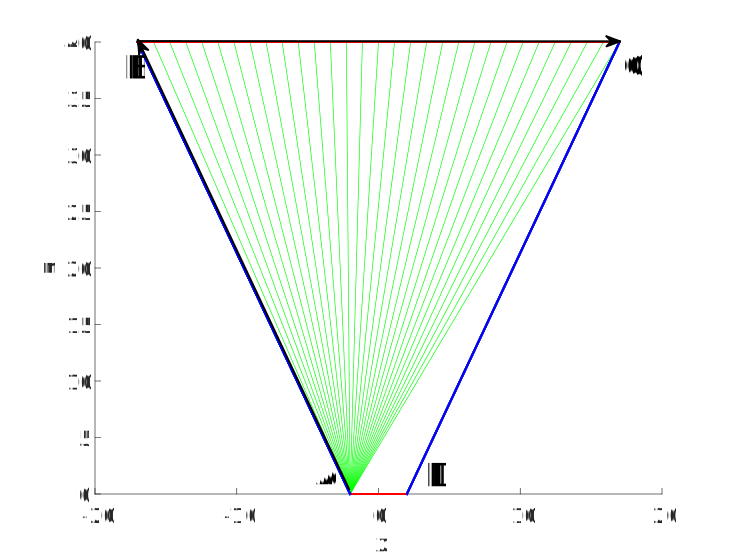
\includegraphics[width=\textwidth]{rays_cup1}
  \caption{Rays that leave the left end point of the source (line $1$) and trace out the target (line $4$).}
  \label{fig:cup1}
\end{subfigure}%
\hfill
\begin{subfigure}{.48\textwidth}
  \centering
  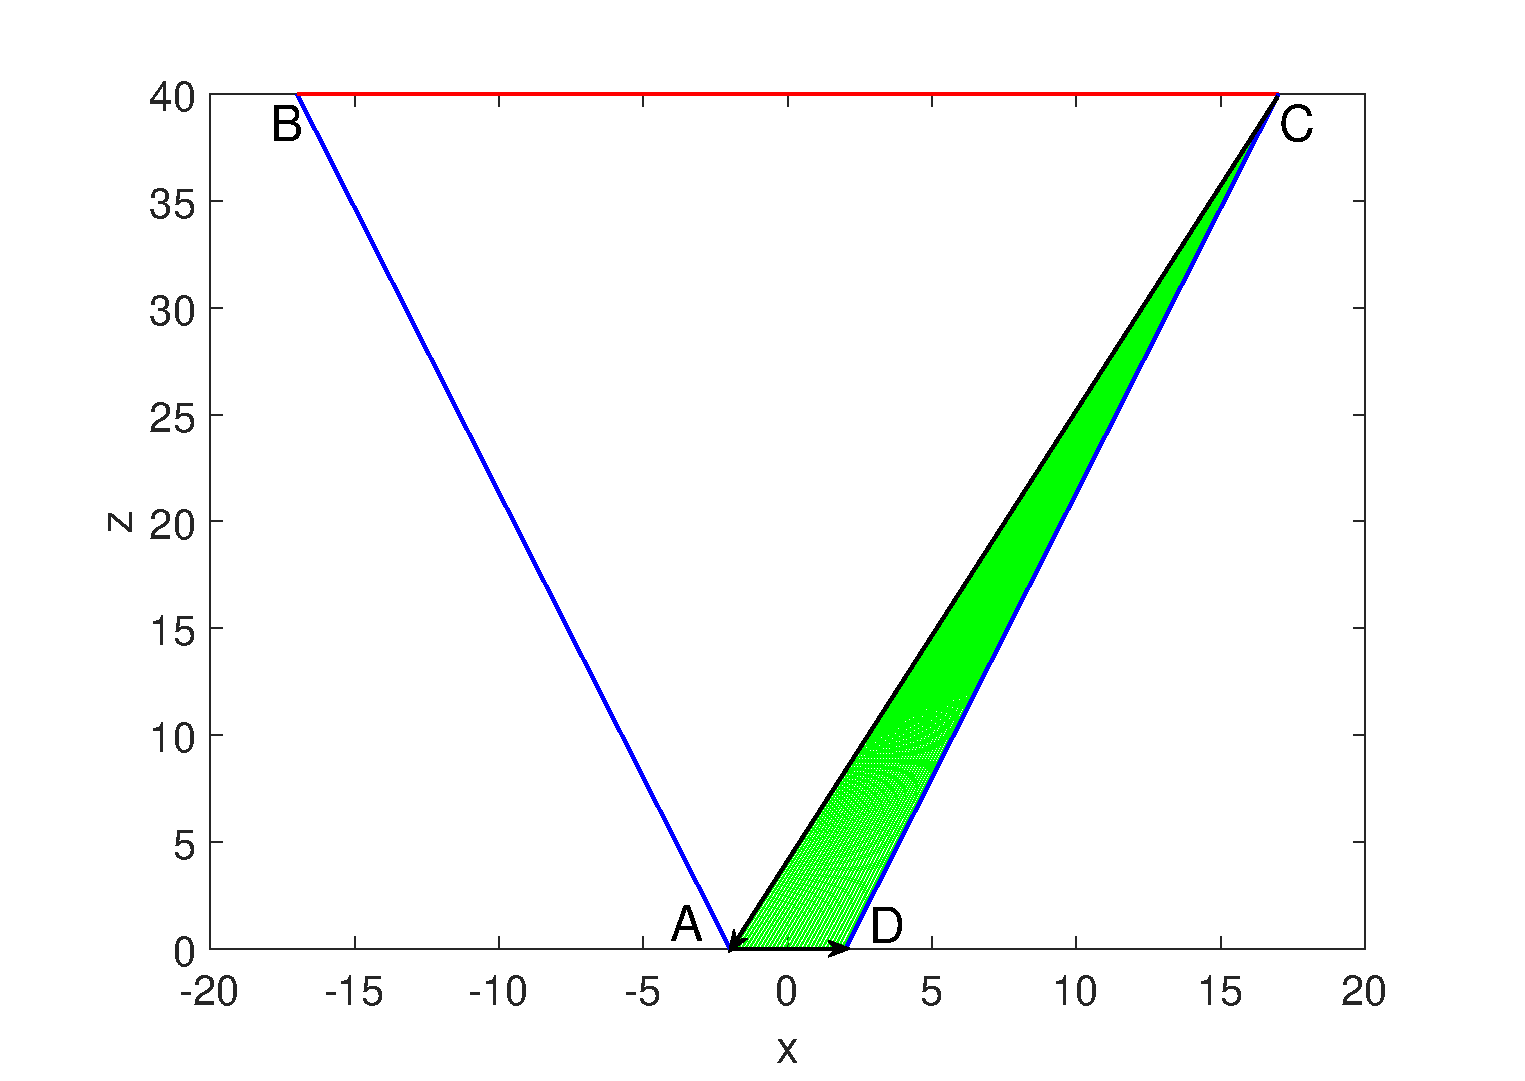
\includegraphics[width=\textwidth]{rays_cup2}
  \caption{Rays that trace out the source (line $1$) and hit the right end point of the target (line $4$).}
  \label{fig:cup2}
\end{subfigure} %
\hfill
\begin{subfigure}{.48\textwidth}
  \centering
  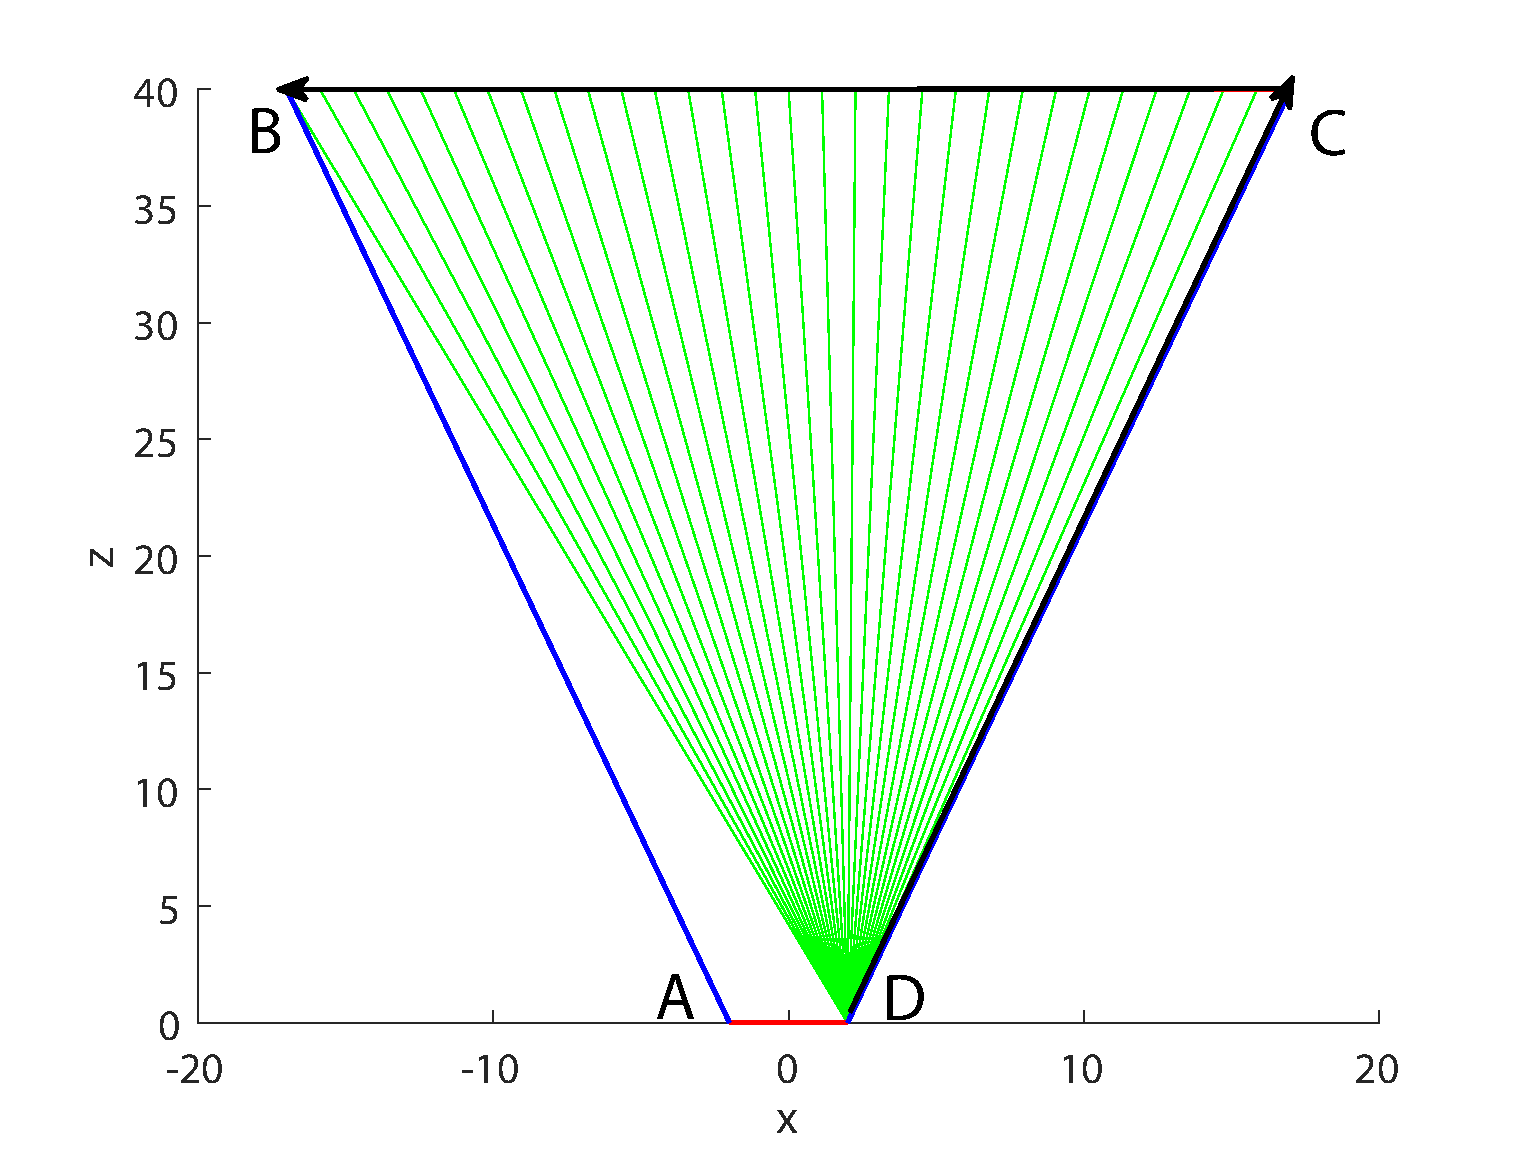
\includegraphics[width = \textwidth]{rays_cup3}
  \caption{Rays that leave the right end point of the source (line $1$) and trace out the target (line $4$).}
  \label{fig:cup3}
\end{subfigure}%
\hfill
\begin{subfigure}{.48\textwidth}
  \centering
  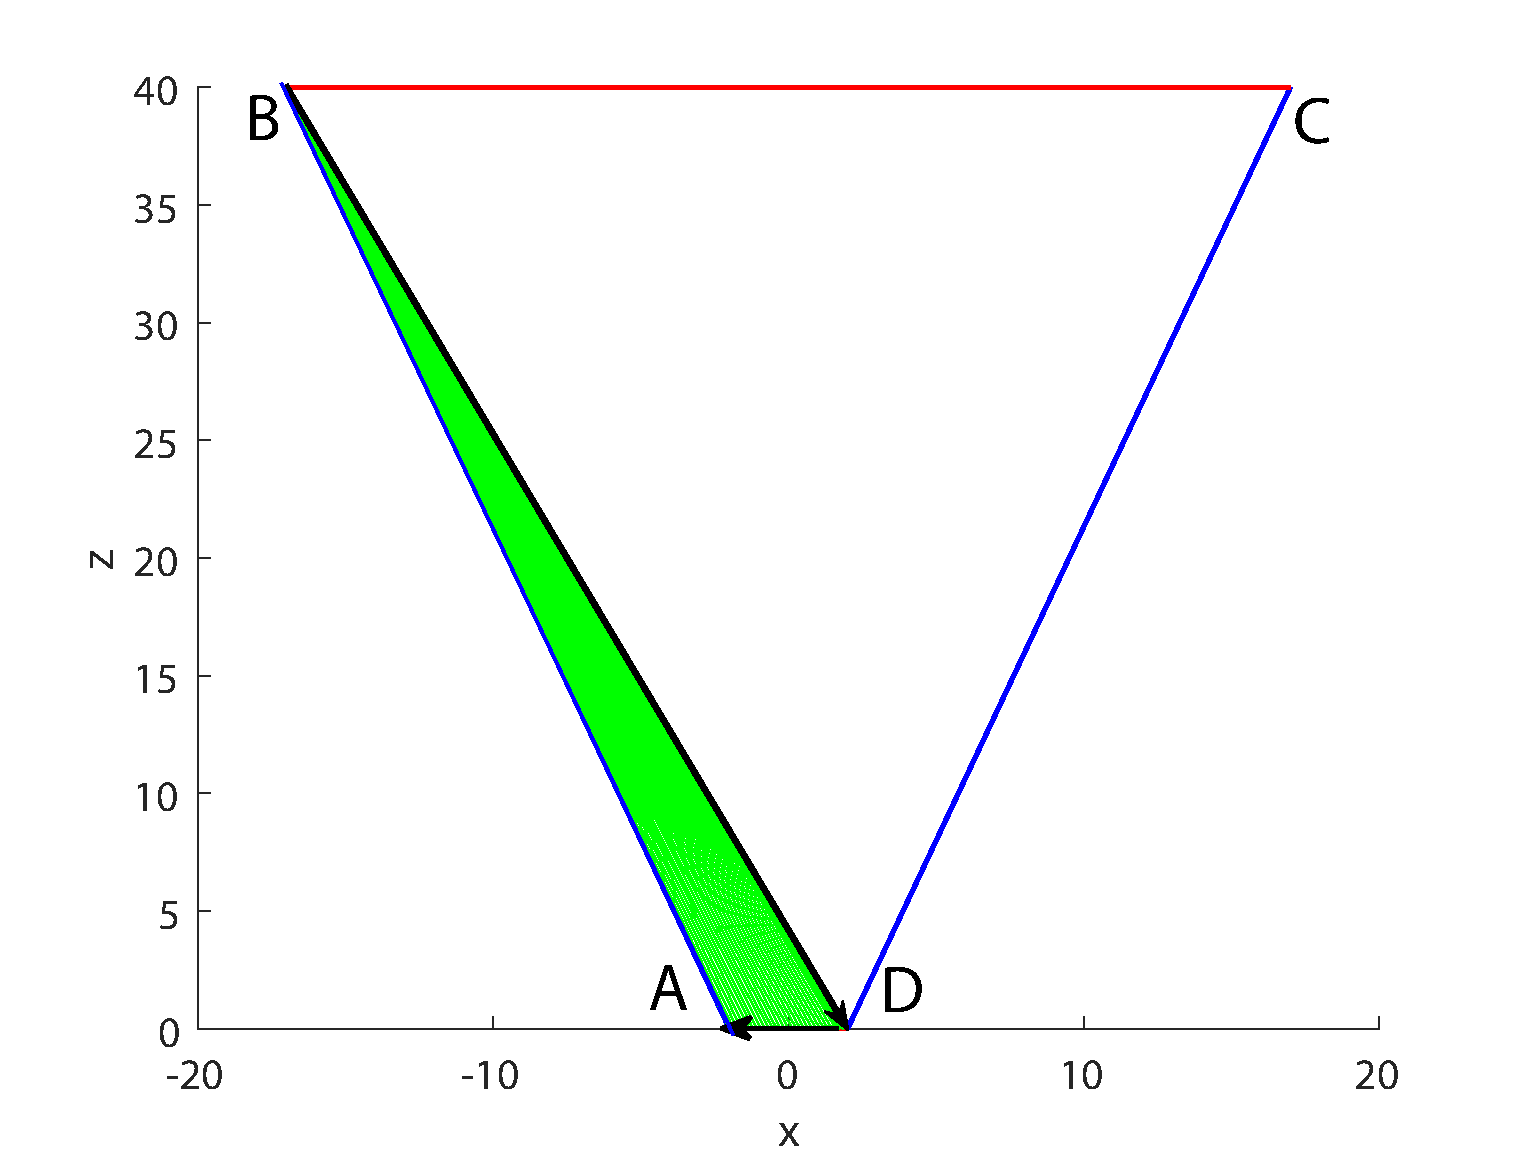
\includegraphics[width=\textwidth]{rays_cup4}
  \caption{Rays that trace out the source (line $1$) and hit the left end point of the target (line $4$).}
  \label{fig:cup4}
\end{subfigure}
\caption{\textbf{Rays located on the boundaries of the regions $\partial$\set{S}{$1$,}{$4$} and $\partial$\set{T}{$4$,}{$1$}}.
$A = (\variabile{x}_{1 \ell}, \variabile{z}_{1, \ell}) =(-2, 0)$ and 
$D = (\variabile{x}_{1, \textrm{r}}, \variabile{z}_{1, \textrm{r}}) = (2, 0)$ 
are the left and right corner points (or end points) of
\point{S} (line $1$), respectively.
$B =  (\variabile{x}_{4, \ell}, \variabile{z}_{4, \ell}) = (-17, 40)$ and $C =  (\variabile{x}_{4, \textrm{r}}, \variabile{z}_{4, \textrm{r}}) = (17 , 40)$, are the left and right corner points (or end points) of \point{T} (line $4$), respectively.}
\label{fig:cups}
\end{figure} \\
 The boundaries $\partial$\set{S}{$1$,}{$4$} and $\partial$\set{T}{$4$,}{$1$} are given in Figs. \ref{fig:S14} and \ref{fig:T411}, respectively.
$\partial$\setbound{S}{$1$,}{$4$}{1} and $\partial$\setbound{T}{$4$,}{$1$}{1} are obtained tracing out line $4$ from
$\variabile{q}^{\textrm{min}} = -\variabile{b}$ to $\variabile{q}^{\textrm{max}} = \variabile{b}$
 by rays leaving $\variabile{q}_{1}^{\textrm{min}}= -\variabile{a}$ with varying $\variabile{p}_1$, these rays are shown in Fig. \ref{fig:cup1}, and the boundary segments
 $\partial$\setbound{S}{$1$,}{$4$}{1} and $\partial$\setbound{T}{$4$,}{$1$}{1} are the orange line segments labeled with \const{c}. 
 $\partial$\setbound{S}{$1$,}{$4$}{2} and $\partial$\setbound{T}{$4$,}{$1$}{2} are given tracing out line $1$ from
 $\variabile{q}_{1, \textrm{min}}= -\variabile{a}$ to $\variabile{q}_{1, \textrm{max}}= \variabile{a}$
 with varying $\variabile{p}_1$, such that all rays hit $\variabile{q}_{\textrm{max}} = \variabile{b}$, these rays are shown in Fig. \ref{fig:cup2}, the boundary segments
 $\partial$\setbound{S}{$1$,}{$4$}{2} and $\partial$\setbound{T}{$4$,}{$1$}{2} are depicted in blue (lines segments labeled with \const{d}).
 Likewise, $\partial$\setbound{S}{$1$,}{$4$}{3} and $\partial$\setbound{T}{$4$,}{$1$}{3} are obtained tracing out line $4$ from
$\variabile{q}_{\textrm{max}}= \variabile{b}$ to $\variabile{q}_{\textrm{min}}= -\variabile{b}$ 
 by rays leaving $\variabile{q}_{1, \textrm{max}}=\variabile{x}_{1, \textrm{r}} = \variabile{a}$ with varying $\variabile{p}_{1}$. These rays are shown in Fig. \ref{fig:cup3}, 
 $\partial$\setbound{S}{$1$,}{$4$}{3} and $\partial$\setbound{T}{$4$,}{$1$}{3} are the red line segments labeled with \const{e}.
  Finally, $\partial$\setbound{S}{$1$,}{$4$}{4} and $\partial$\setbound{T}{$4$,}{$1$}{4} are given tracing out line $1$ from
$\variabile{q}_{1, \textrm{max}} = \variabile{a}$ to  $\variabile{q}_{1, \textrm{min}} = -\variabile{a}$ 
 with varying $\variabile{p}_{1}$, such that all rays hit $\variabile{q}_{\textrm{min}} = -\variabile{b}$, these rays are shown in Fig. \ref{fig:cup4}, 
 $\partial$\setbound{S}{$1$,}{$4$}{4} and $\partial$\setbound{T}{$4$,}{$1$}{4} are the green lines segments labeled with \const{f}. 
We remind that we use the notation $(\variabile{x}, \variabile{z})$ for the Cartesian coordinates system of real space, while phase space has $(\variabile{q}, \variabile{p})$ coordinates. 
It is worth noting that  $\variabile{q}_{1, \textrm{min}}=\variabile{x}_{1, \ell}$,  $\variabile{q}_{1, \textrm{max}}=\variabile{x}_{1, \textrm{r}}$,  
$\variabile{q}_{\textrm{min}}=\variabile{x}_{4, \ell}$ and  $\variabile{q}_{\textrm{max}}=\variabile{x}_{4, \textrm{r}}$.\\ \indent
 For the two-faceted cup there is an analytic expression for every line segment $\partial\mbox{\setbound{S}{\lineai,}{\lineak}{\variabile{\,m}}}$ and
 $\partial\mbox{\setbound{T}{\lineak,}{\lineai}{\variabile{\,m}}}$ in Eq. (\ref{eq:analytic_boundaries}) with $\variabile{m}\in\{1, \cdots, 4\}$.
 For instance, the rays on the boundaries $\partial\mbox{\setbound{S}{\lineai,}{\lineak}{\,1}}$ and $\partial \mbox{\setbound{T}{\lineak,}{\lineai}{\,1}}$
  are parameterized in the (\variabile{x}, \variabile{z})-plane by
 \begin{equation}
\label{extremes_rays}
\vect{r}_{\variabile{\lineai}, \variabile{\lineak}}(\variabile{t})=
\left( \begin{array}{cc}
\variabile{x}_{\variabile{\lineak}, \ell}-\variabile{x}_{\variabile{\lineai}, \ell}+t(\variabile{x}_{\variabile{\lineak}, \textrm{r}}-\variabile{x}_{\variabile{\lineak}, \ell}) \\
\variabile{z}_{\variabile{\lineak}, \ell}-\variabile{z}_{\variabile{\lineai}, \ell}+t(\variabile{z}_{\variabile{\lineak}, \textrm{r}}-\variabile{z}_{\variabile{\lineak},\ell})
\end{array} \right) \qquad \quad 0\leq t\leq 1\,.
\end{equation}
 These rays are located on a vertical line segment in \set{S}{\lineai}{} as only the $\mbox{\variabile{p}}_{\variabile{\lineai}}$-coordinate changes and on a curved line in 
\set{T}{\lineak}{}
  as both the target position and direction vary. The analytic expressions for $\partial \mbox{\setbound{S}{\lineai,}{\lineak}{\,1}}$ and $\partial \mbox{\setbound{T}{\lineak,}{\lineai}{\,1}}$ are
\begin{equation}
\label{S_boundary}
\partial \mbox{\setbound{S}{\lineai,}{\lineak}{1}}(\variabile{t})= \bigg\{ (\variabile{q}_{\variabile{\lineai}}, \variabile{p}_{\variabile{\lineai}}) = \Big(\variabile{q}_{\variabile{\lineai}, \textrm{min}},
|\boldsymbol{\nu}_{\variabile{\lineai}}\times \hat{\vect{r}}_{\variabile{\lineai}, \variabile{\lineak}}(\variabile{t})|
\Big), \bigg\}
\end{equation}
\begin{equation}
\label{T_boundary}
\partial\mbox{\setbound{T}{\lineak,}{\lineai}{\,1}}(\variabile{t})=\bigg\{(\variabile{q}_{\variabile{\lineak}}, \variabile{p}_{\variabile{\lineak}}) =
\Big(\variabile{q}_{\variabile{\lineak}, \textrm{max}}-\variabile{q}_{\variabile{\lineai}, \textrm{min}}+t(\variabile{q}_{\variabile{\lineak}, \textrm{max}}-\variabile{q}_{\variabile{\lineak},\textrm{min}}),
|\boldsymbol{\nu}_{\variabile{\lineak}}\times \hat{\vect{r}}_{\variabile{\lineai}, \variabile{\lineak}}(\variabile{t})|\Big) \bigg\}\,,
\end{equation}
where we have indicated with $\hat{\vect{r}}_{\variabile{\lineai}, \variabile{\lineak}}(\variabile{t})$ the normalization of the ray in Eq. ($\ref{extremes_rays}$) and,
 $ \boldsymbol{\nu}_\variabile{\lineai}$ and $\boldsymbol{\nu}_\variabile{\lineak}$ are the normalized inward normals to lines $\variabile{\lineai}$ and $\variabile{\lineak}$, respectively.
 Note that,  $\sin{\tau_\variabile{\lineai}} = |\nu_{\variabile{\lineai}}\times \hat{\vect{r}}_{\variabile{\lineai}, \variabile{\lineak}}(\variabile{t})|$ and $\sin{\tau_\variabile{\lineak}} = |\nu_{\variabile{\lineak}}\times \hat{\vect{r}}_{\variabile{\lineai}, \variabile{\lineak}}(\variabile{t})|$.
 \begin{figure}
 \begin{minipage}[]{.48\textwidth}
   \centering
   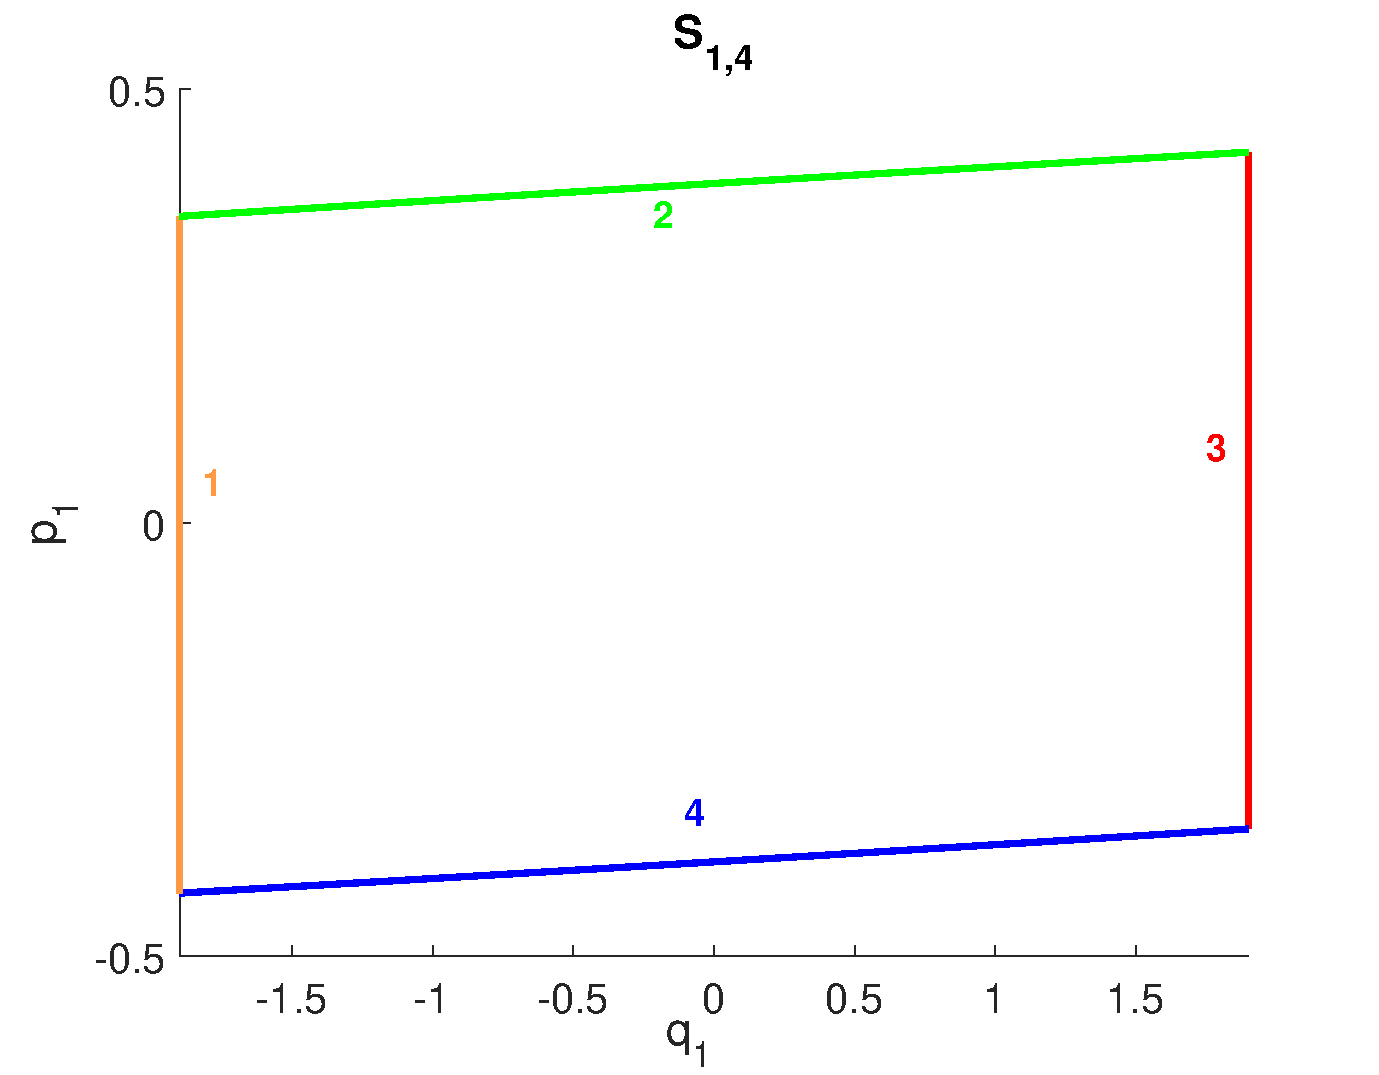
\includegraphics[width=\textwidth]{S141}
   \caption{Source phase space of line $1$.
   Boundary of the region \set{S}{$1$,}{$4$}.}
   \label{fig:S14}
 \end{minipage}\hfill
  \begin{minipage}[]{0.48\textwidth}
  \centering
   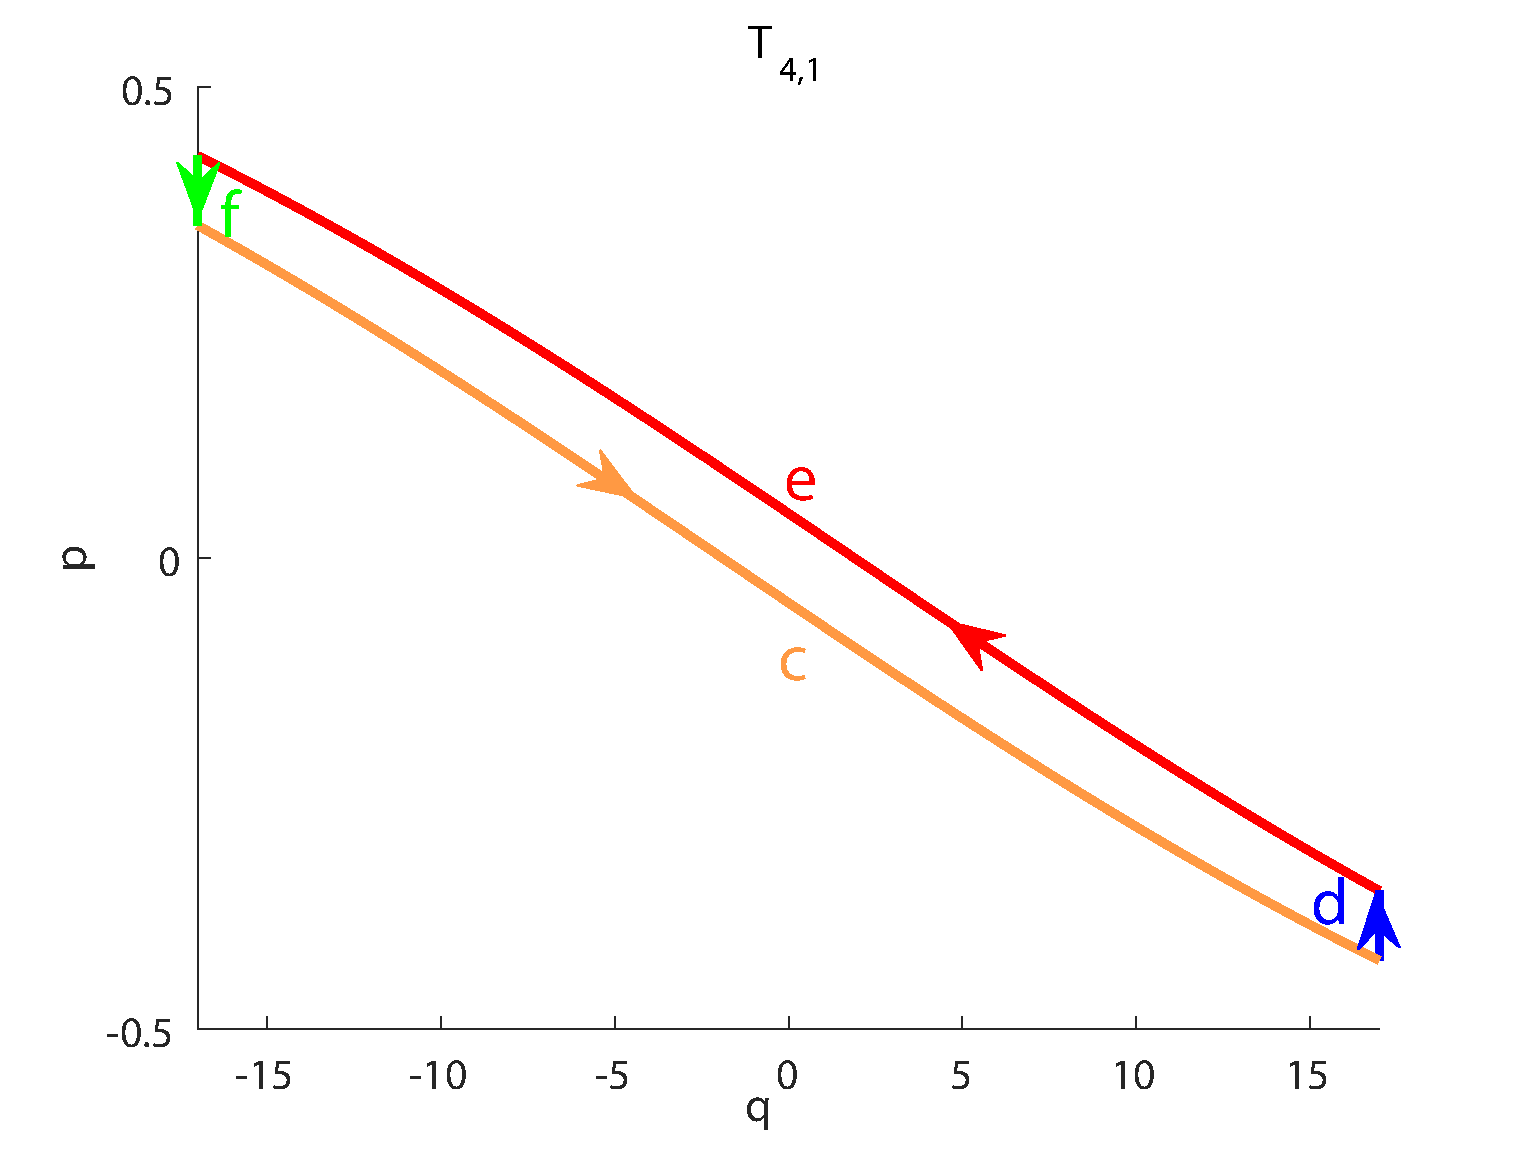
\includegraphics[width=\textwidth]{T411}
   \caption{Target phase space of line $4$.
    Boundary of the region \set{T}{$4$,}{$1$}.}
    \label{fig:T411}
 \end{minipage}
 \end{figure}
 Likewise, the boundaries $\partial$\setbound{S}{\lineai,}{\lineak}{\variabile{\,m}} and
 $\partial$\setbound{T}{\lineak,}{\lineai}{\variabile{\,m}} are calculated for every $\variabile{m}\in\{2,3,4\}$ and $\partial$\set{S}{\lineai,}{\lineak} and $\partial$\set{T}{\lineak,}{\lineai} are found using Eq. (\ref{eq:analytic_boundaries}). \\
 \begin{figure}
 \begin{minipage}[]{.43\textwidth}
   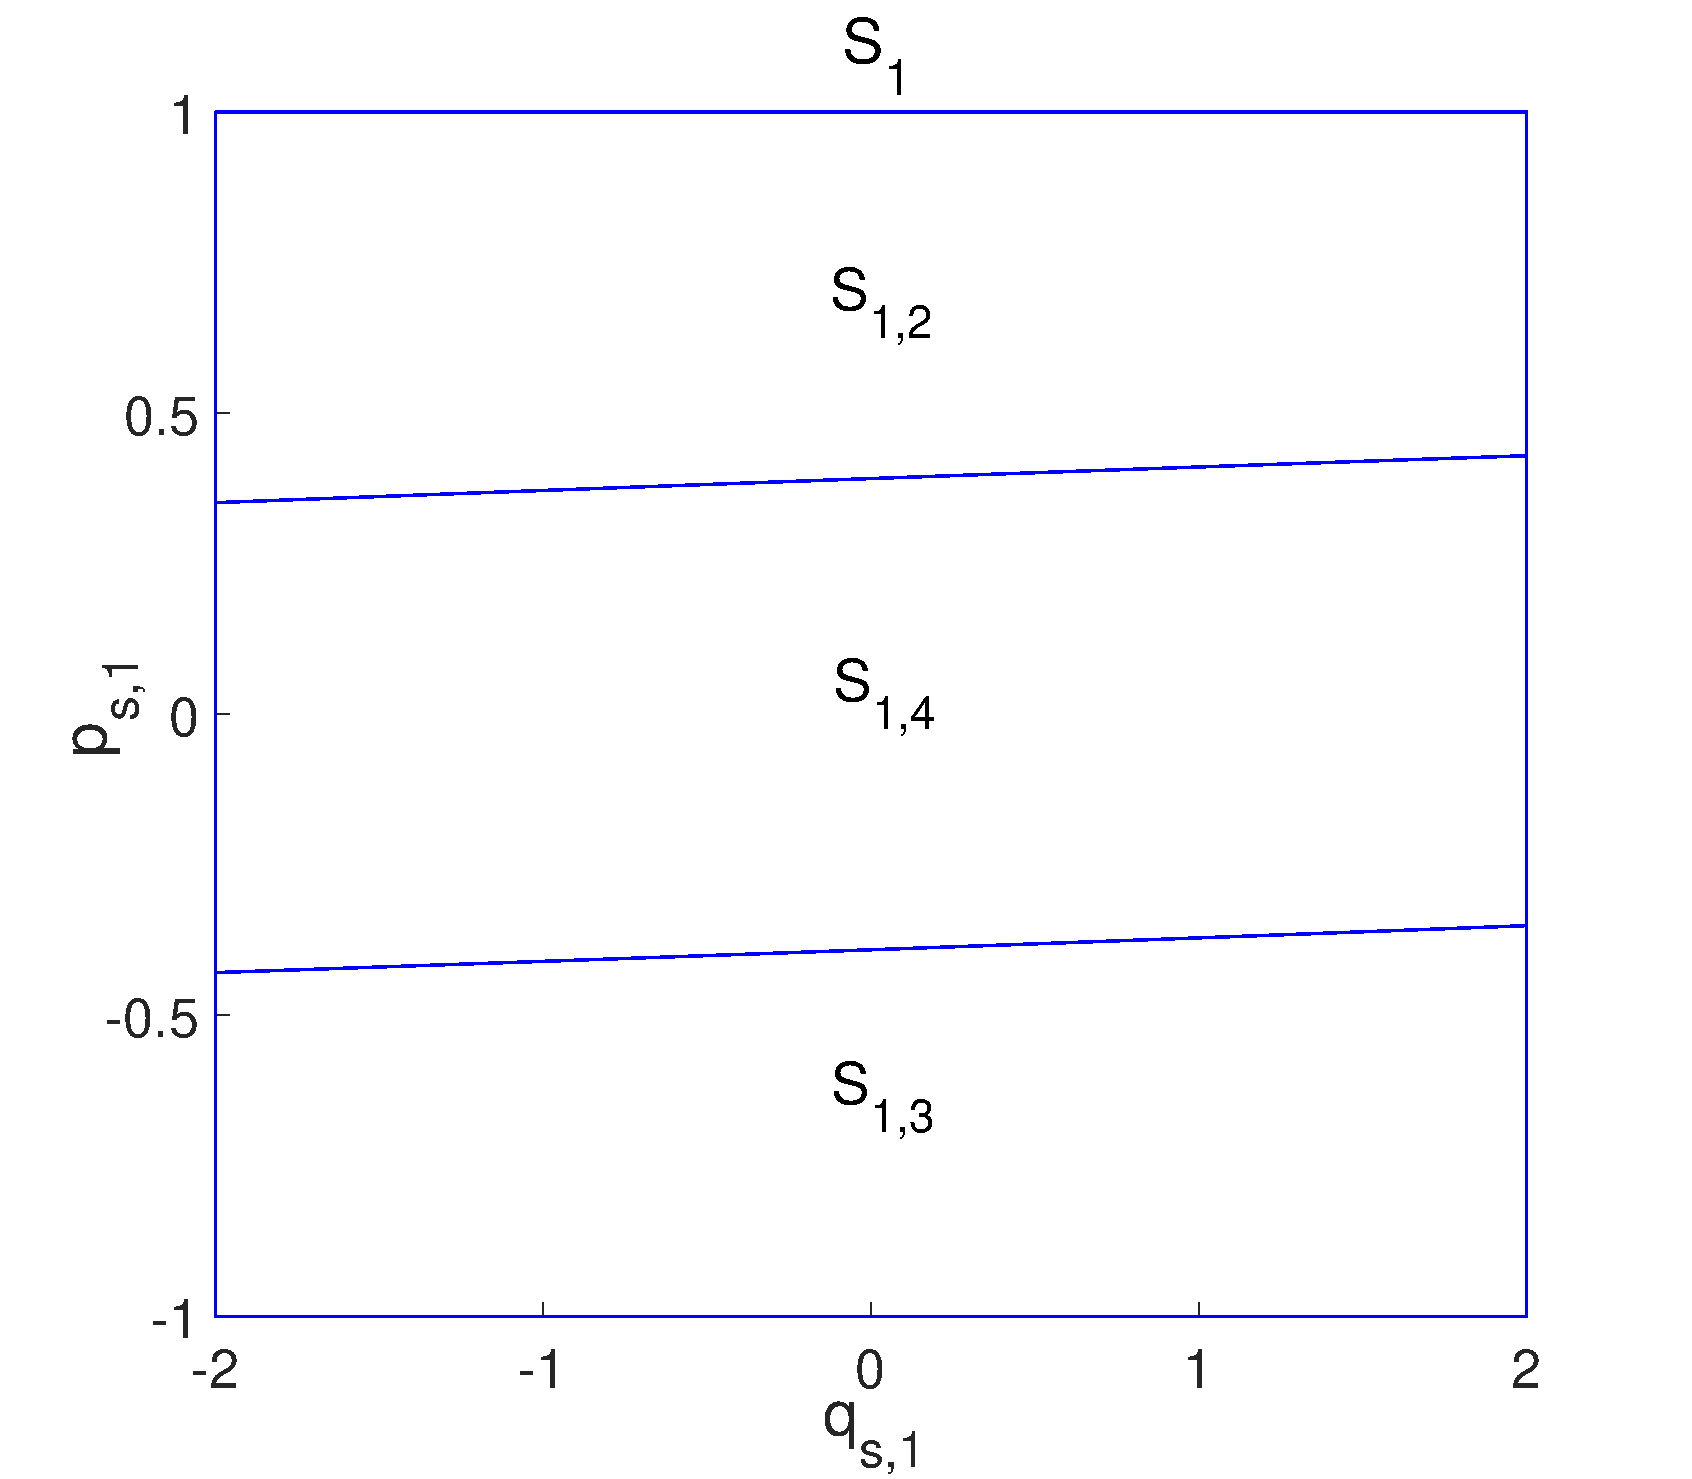
\includegraphics[width=\textwidth]{S1}
\caption{\footnotesize{The PS $\mbox{\set{S}{$1$}{}}$ of line $1$ is partitioned into regions $(\mbox{\set{S}{$1$,}{\lineaj}})_{\variabile{\lineaj} = 2,3,4}$
   formed by rays that leave line $1$ and hit line $\textit{\lineaj}$.}}
   \label{fig:S1}
 \end{minipage}
  \begin{minipage}[]{.45\textwidth}
  \centering
   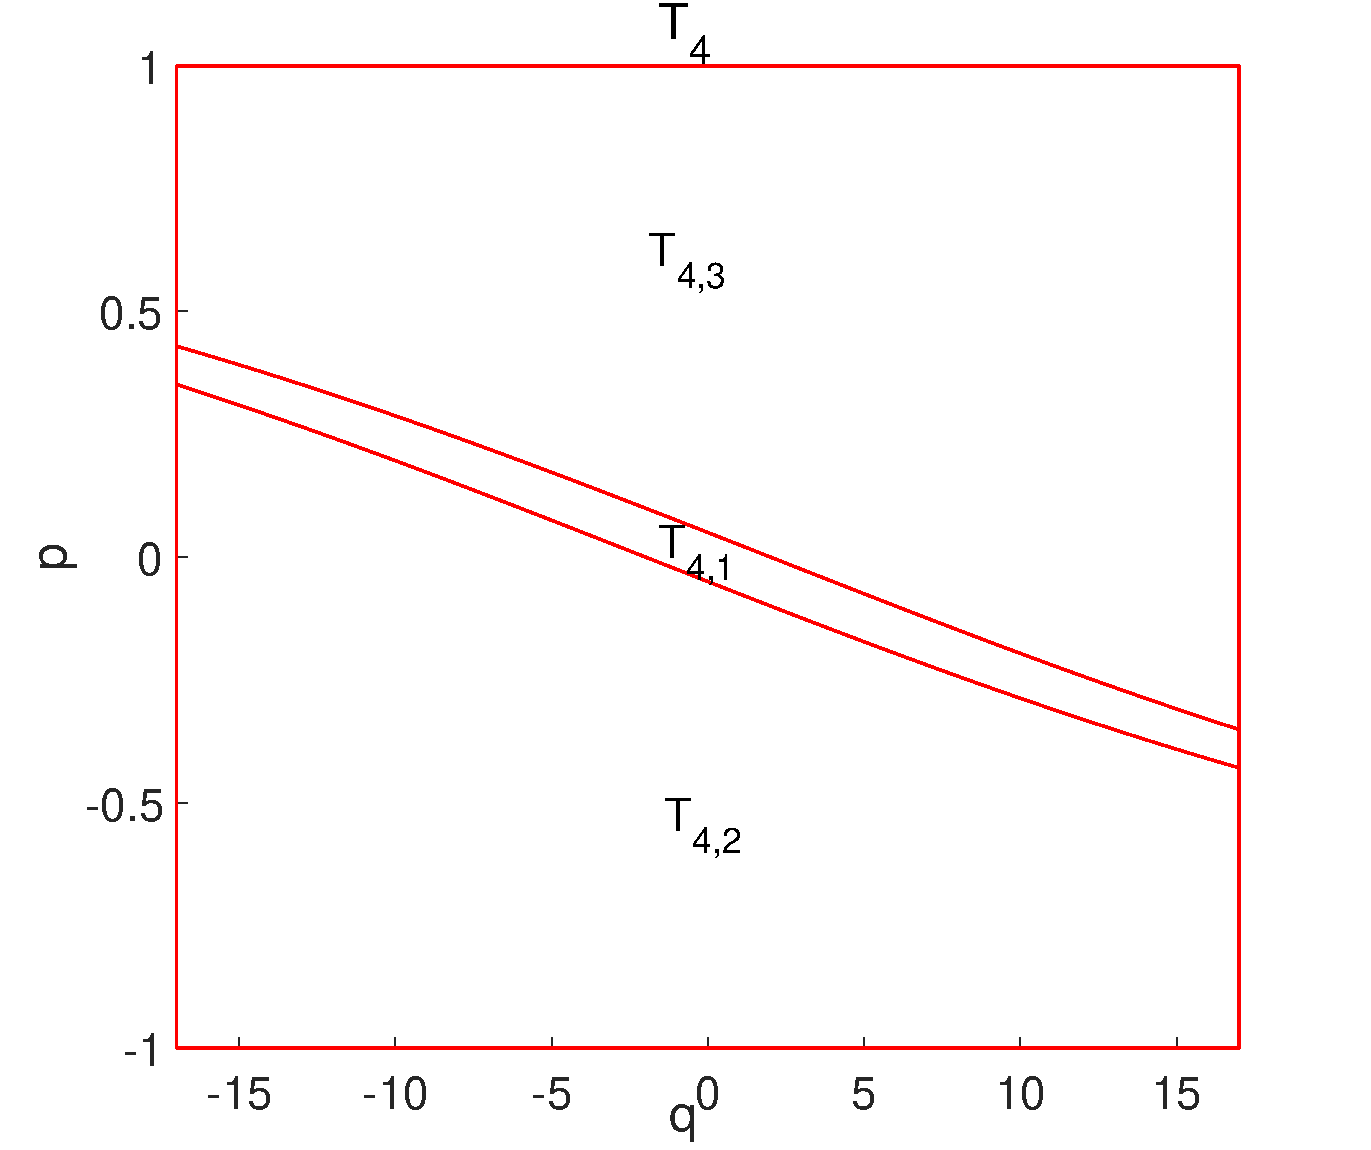
\includegraphics[width=\textwidth]{T4b}
   \caption{\footnotesize{The PS $\mbox{\set{T}{$4$}{}}$ of line $4$ is partitioned into regions $(\mbox{\set{T}{$4$,}{\lineak}})_{\variabile{\lineak} = 1,2,3}$
   formed by rays that leave line $\textit{\lineak}$ and hit line $4$.}}
   \label{fig:T4b}
 \end{minipage}
\begin{minipage}[]{.43\textwidth}
\centering
   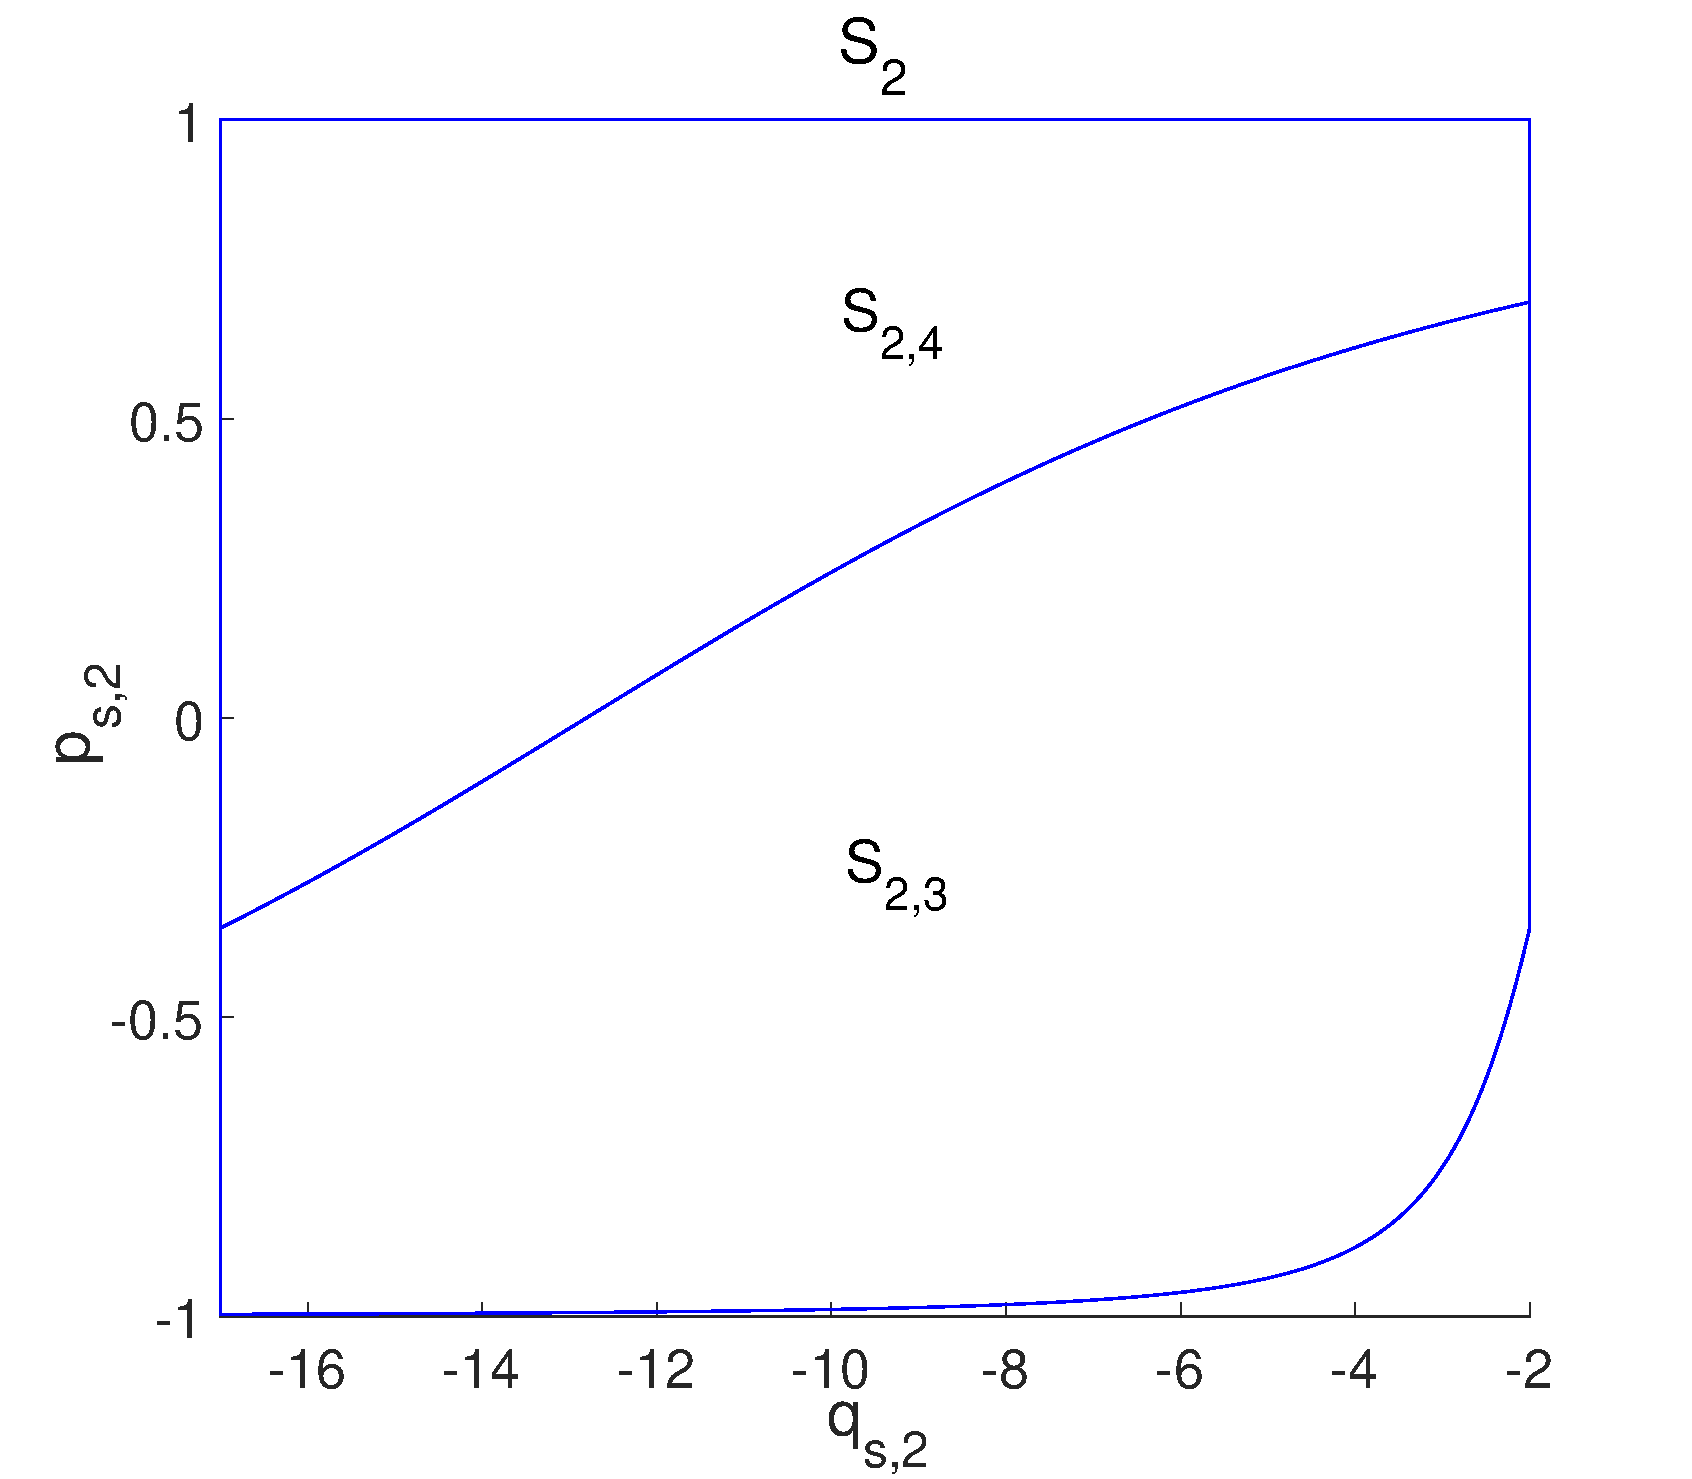
\includegraphics[width=\textwidth]{S2}
\caption{\footnotesize{The PS $\mbox{\set{S}{$2$}{}}$ of line $2$ is partitioned into regions $(\mbox{\set{S}{$2$,}{\lineaj}})_{\variabile{\lineaj} = 3,4}$
  formed by rays that leave line $2$ and hit line $\variabile{\lineaj}$.}} 
 \end{minipage}
 \begin{minipage}[]{.43\textwidth}
 \centering
   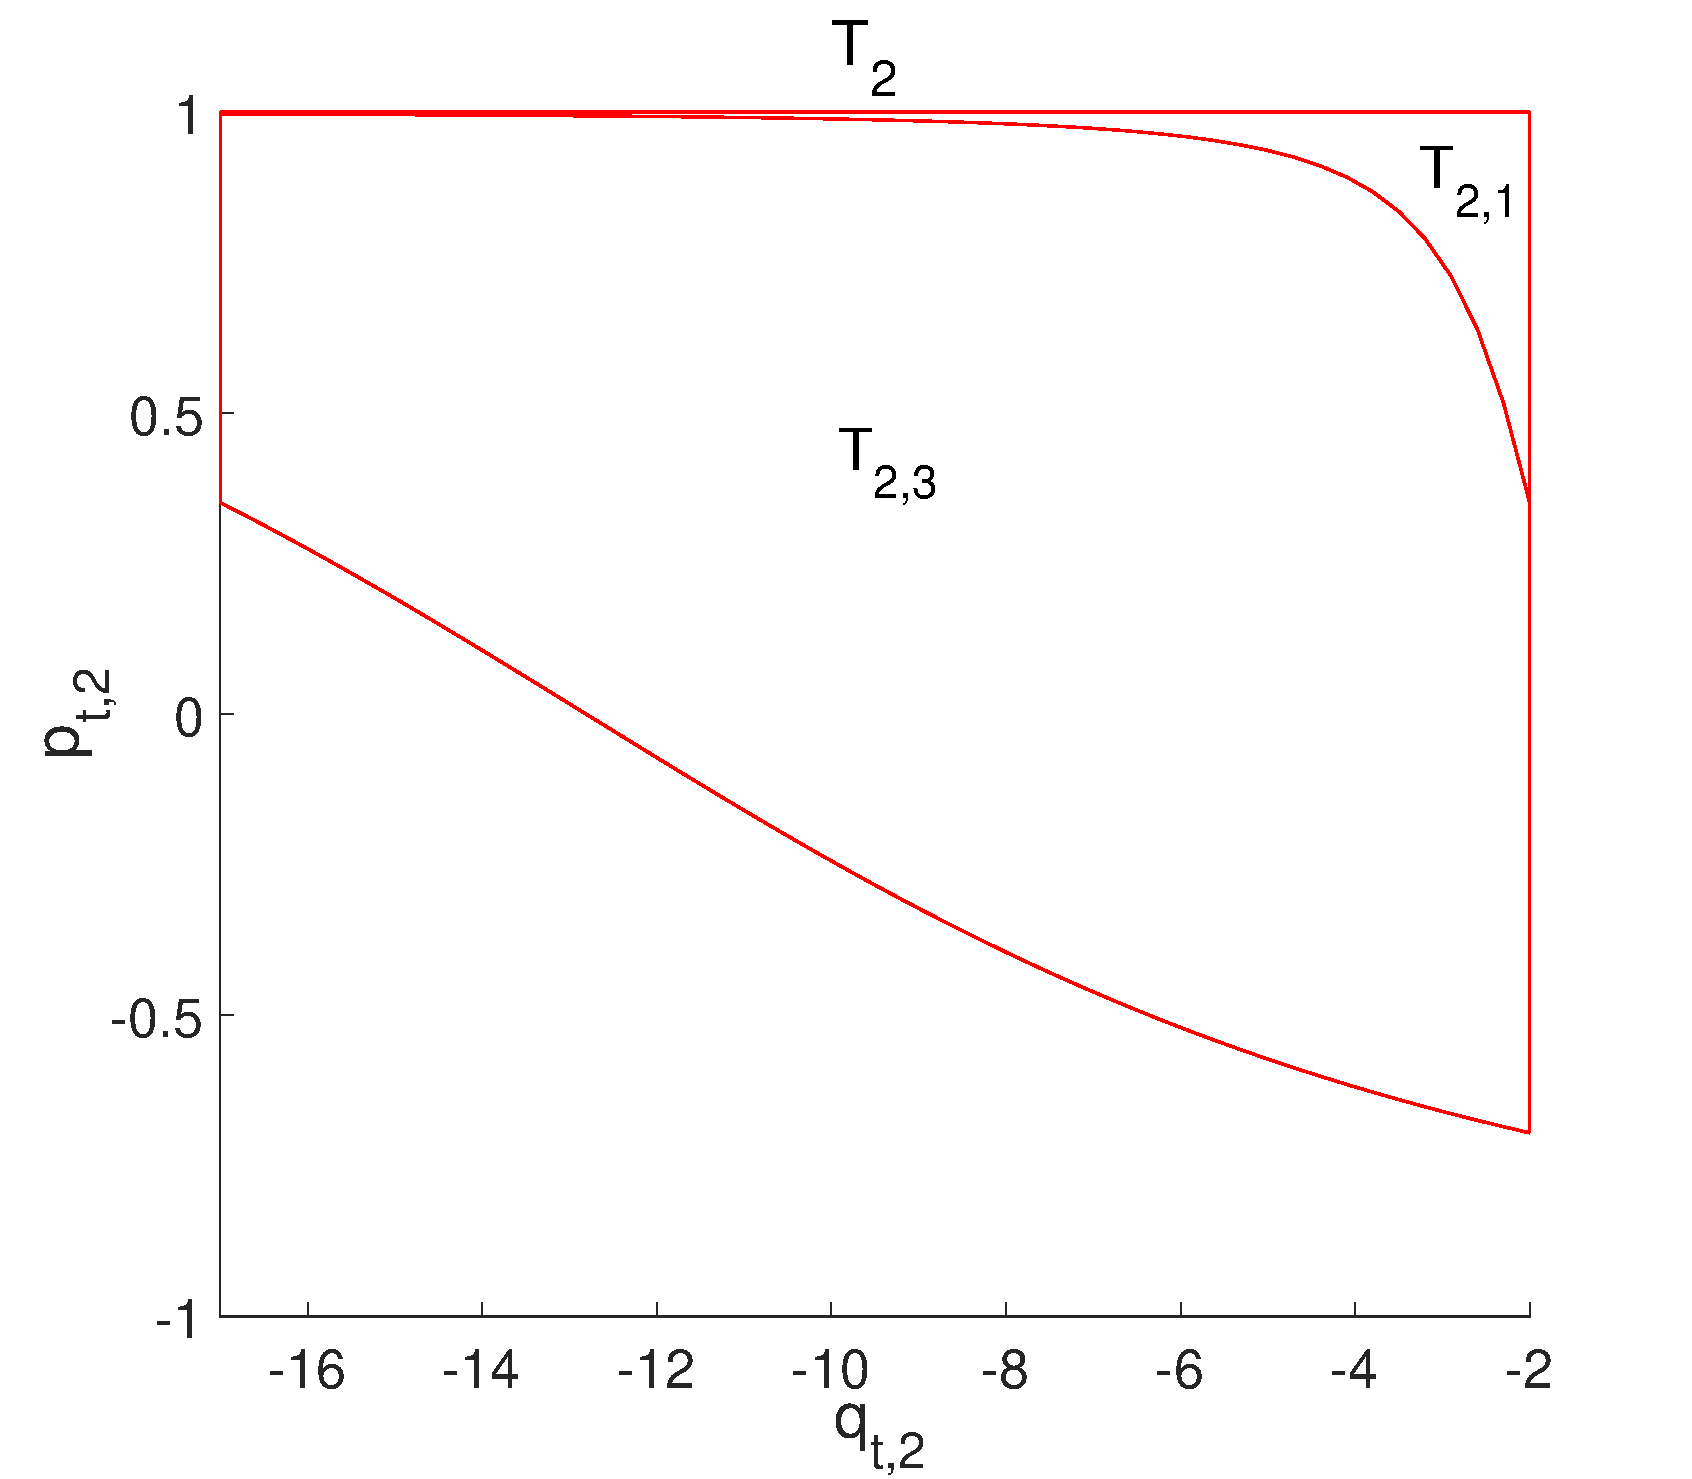
\includegraphics[width=\textwidth]{T2b}
\caption{\footnotesize{The PS $\mbox{\set{T}{$2$}{}}$ of line $2$ is partitioned into regions $(\mbox{\set{T}{$2$,}{\lineak}})_{\variabile{\lineak} = 1,3}$
formed by rays that leave line $\variabile{\lineak}$ and hit line $2$. }} 
 \end{minipage}
 \begin{minipage}[]{.43\textwidth}
 \centering
   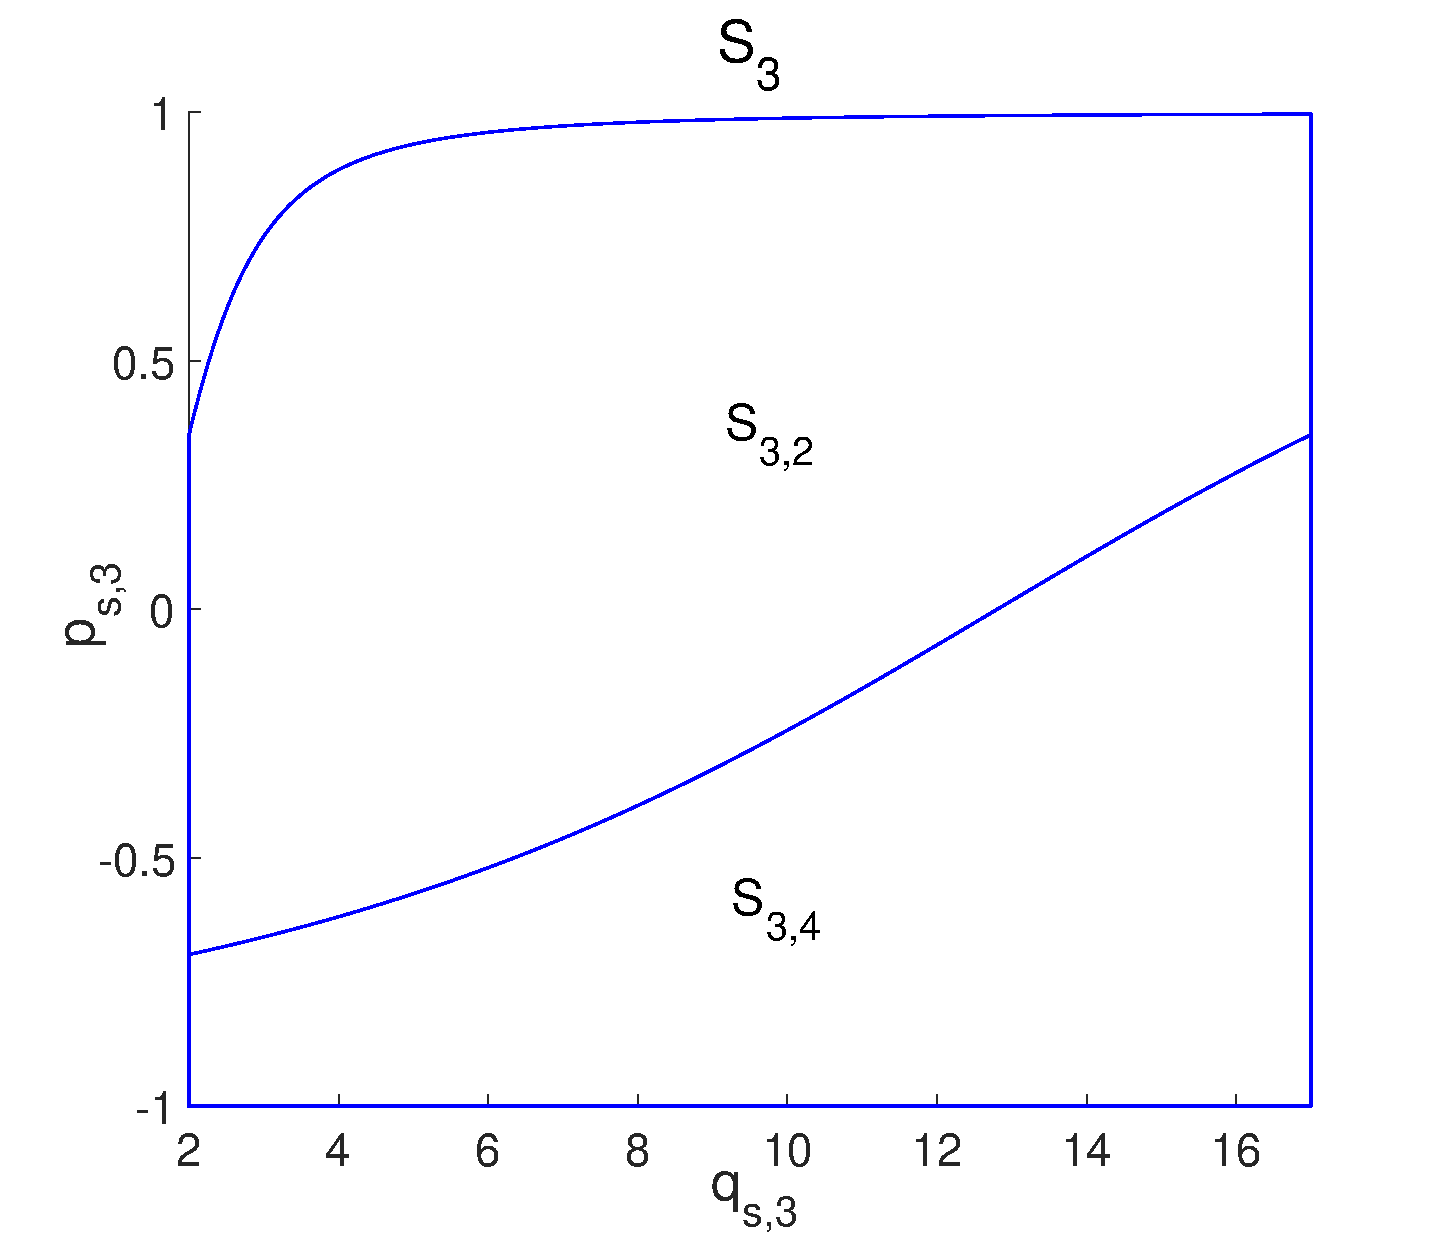
\includegraphics[width=\textwidth]{S3}
   \caption{\footnotesize{The PS $\mbox{\set{S}{$3$}{}}$ of line $3$ is partitioned into regions
   $(\mbox{\set{S}{$3$,}{\lineaj}})_{\variabile{\lineaj} = 2,4}$ formed by rays that leave line $3$ and hit line $\variabile{\lineaj}$. }} 
 \end{minipage}
 \hspace{1.7cm}
 \begin{minipage}[]{.43\textwidth}
 \centering
   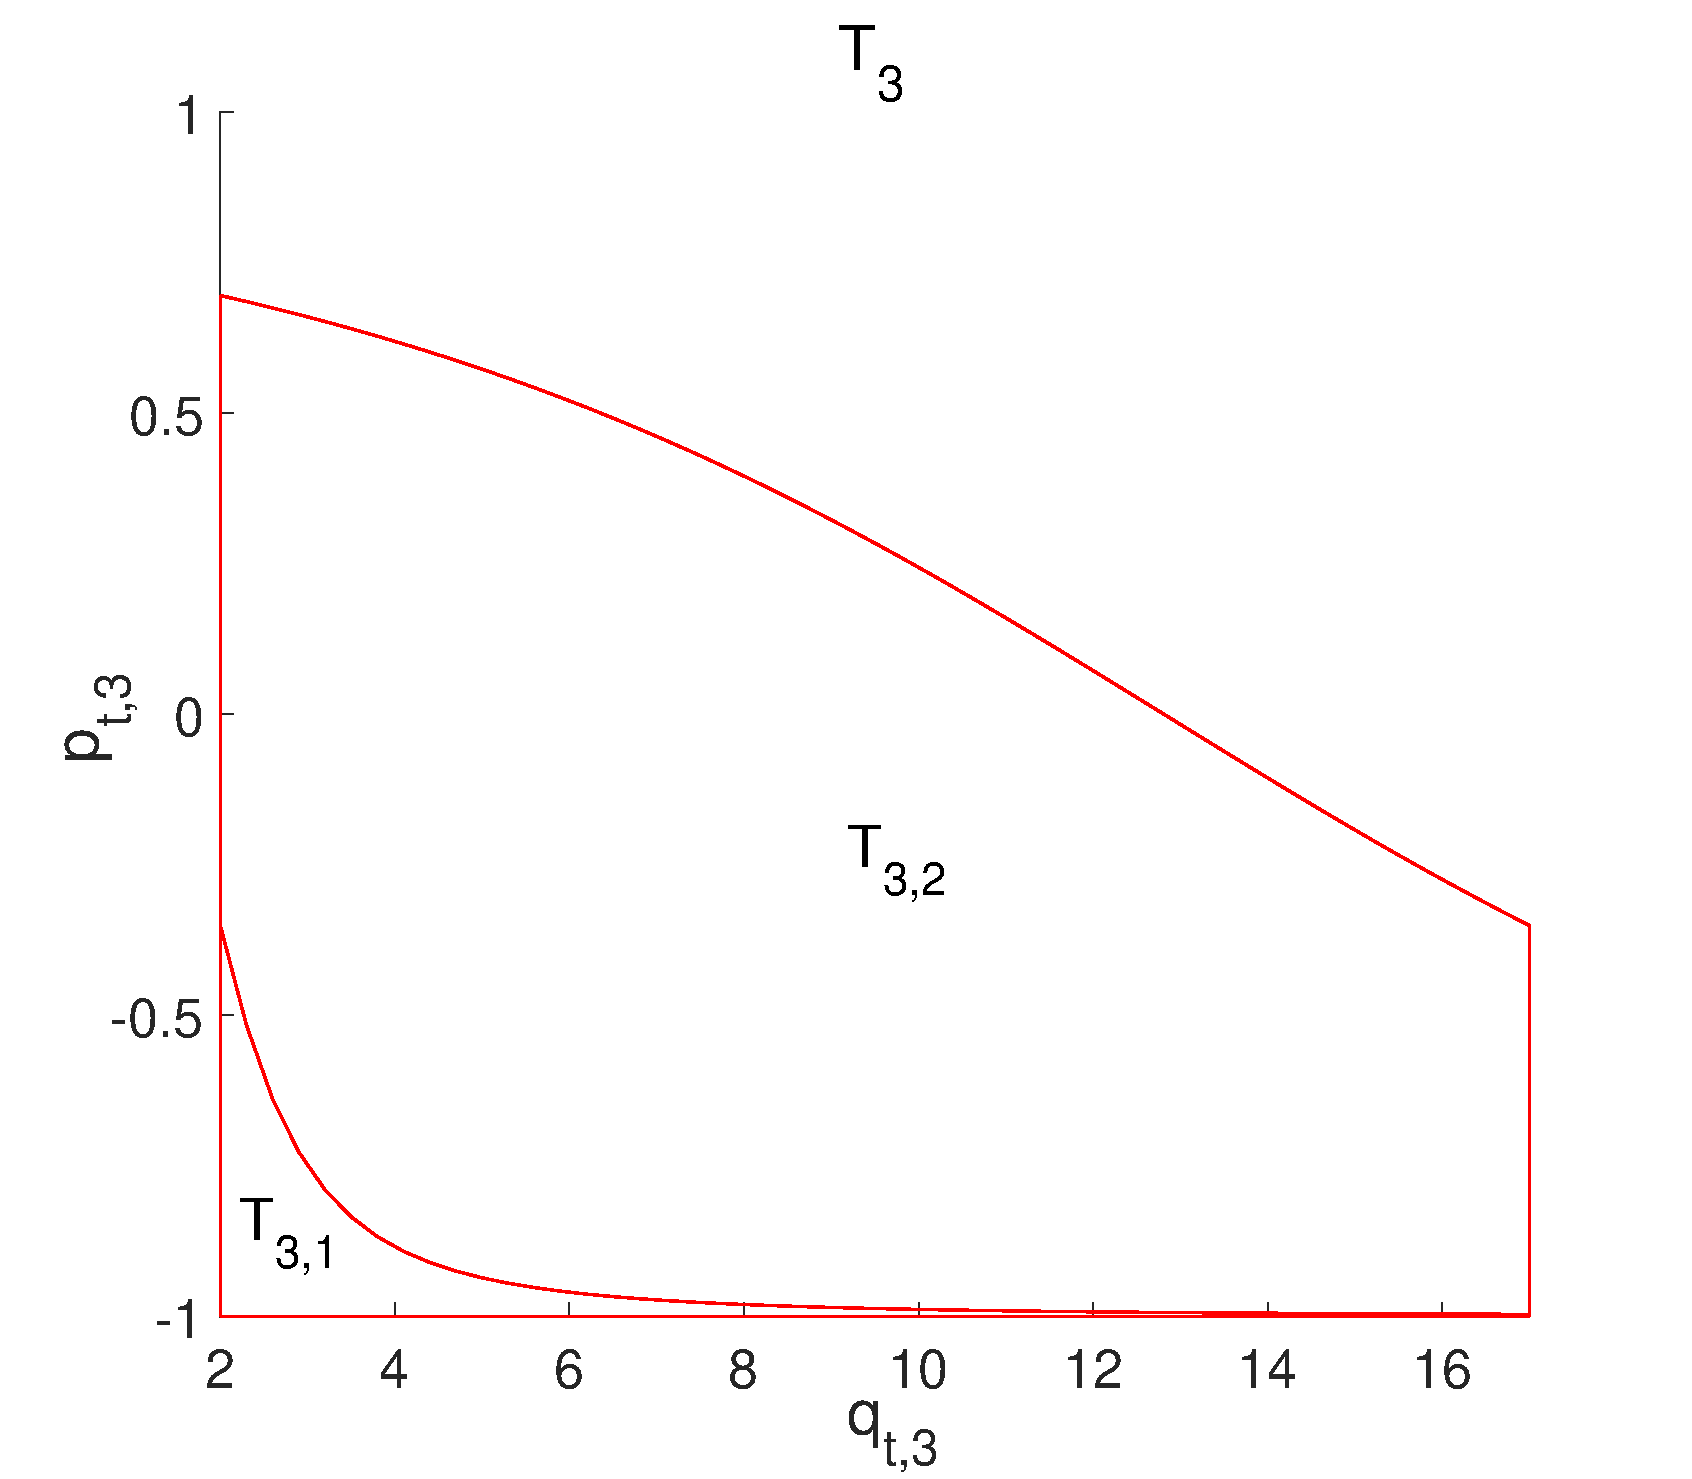
\includegraphics[width=\textwidth]{T3_b}
  \caption{\footnotesize{The PS $\mbox{\set{T}{$3$}{}}$ of line $3$ is partitioned into regions $(\mbox{\set{T}{$3$,}{\lineak}})_{\variabile{\lineak} = 1,2}$
   formed by rays that leave line $\variabile{\lineak}$ and hit line $3$.}} 
\label{fig:T3}
 \end{minipage}
\end{figure}
\indent In Figs. $\ref{fig:S1}-\ref{fig:T3}$,  $(\partial \mbox{\set{S}{\lineai,}{\lineaj}})_{\variabile{\lineai}\neq\variabile{\lineaj}=2, 3, 4}$ and $(\partial \mbox{\set{T}{\lineai,}{\lineak}})_{\variabile{\lineai}\neq\variabile{\lineak}=1, 2, 3}$ are depicted in blue and red, respectively. The source and target PS of lines $2$ and $3$ have some empty regions. 
These parts correspond to the regions formed by the rays that either go back to the source or are emitted from the target. These regions are not taken into account, see Eq. (\ref{eq:analytic_boundaries}). We observe that, because of the symmetry of the optical system, \set{S}{$3$}{} is the mirror image of \set{S}{$2$}{} after reflection in the central point 
$(\variabile{q}, \variabile{p}) = (-9.5, 0)$ and translation from $(\variabile{q}, \variabile{p})\rightarrow(\variabile{q}+19, \variabile{p})$. Likewise \set{T}{$3$}{} is the mirror image of \set{S}{$2$}{} after the same reflection and translation.
%In the next section, we show how the phase spaces are related to each other and we define the target photometric variables on \set{T}{$4$}{}.
\subsection{The structure of the algorithm}
In this section we explain how to compute the target photometric variables in PS.
The intensity $I$ along a given direction $\variabile{p}\in [-1,1]$ in target phase space \set{T}{$4$}{} is a function of the luminance $L(\variabile{q}, \variabile{p})$ defined as in Equation (\ref{eq:PSintensity}). For the two-faceted cup, it becomes:
\begin{equation}\label{I(eta)}
I_{\textrm{PS}}(\variabile{p}) = \int_{-\variabile{b}}^{\variabile{b}} L(\variabile{q},\variabile{p}) \textrm{d}\variabile{q}\,.
\end{equation}
The parts of \set{T}{$4$}{} that are illuminated by \set{S}{$1$}{} correspond to parts with positive luminance, for the other parts the luminance is equal to zero.
Assuming positive luminance on \point{S}, the following relations hold:
\begin{subequations}\label{LT4}
\begin{align}
L(\variabile{q}, \variabile{p})&>0 \qquad \quad \forall (\variabile{q}, \variabile{p})\in \mbox{\set{T}{$4$,}{$1$}},\\
L(\variabile{q}, \variabile{p})&\geq 0 \qquad\quad \forall(\variabile{q}, \variabile{p}) \in (\mbox{\set{T}{$4$,}{\lineai}})_{\lineai=2,3}.\label{third}
\end{align}
\end{subequations}
Once a ray leaves the source \point{S} it can hit the reflectors several times before hitting the target \point{T}. To relate \point{S} and \point{T}, a map $\mapnumb{M}_{1,4}$: \set{S}{$1$}{}$\rightarrow$ \set{T}{$4$}{} is introduced such that $\mapnumb{M}_{1,4}(\pos{s,}{$1$},\dir{s,}{$1$})=(\variabile{q},\variabile{p})$. As  not all parts of \set{T}{$4$}{} are illuminated by the source \point{S}, the map
$\mapnumb{M}_{1,4}$ is not surjective.
Therefore, we need to determine the subsets of \set{T}{$4$}{} illuminated by \point{S} corresponding to the regions where the luminance is positive.
To this purpose, we consider two different kinds of maps.
The first map relates the coordinates of the source and the target PS of two \textit{different} lines, we call it the propagation map.
The second map relates the coordinates of the target and the source PS of the \textit{same} line, we call it the reflection map.
In particular, given two lines $\lineai$ and $\lineaj$ with $\lineai\neq\lineaj$, the propagation map $\mapnumb{P}_{\lineai,\lineaj}: \mbox{\set{S}{\lineai,}{\lineaj}}\mapsto$\set{T}{\lineaj,}{\lineai} relates \set{S}{\lineai,}{\lineaj} with \set{T}{\lineaj,}{\lineai} and, it is defined as follows:
 \begin{equation}\label{Pij}
\mapnumb{P}_{\lineai,\lineaj}(\pos{s,}{\lineai},\dir{s,}{\lineai})=(\pos{t,}{\lineaj},\dir{t,}{\lineaj}),
\end{equation}
where $\pos{t,}{\lineaj}$ is given by the \variabile{x}-coordinate of the intersection point between the ray and line $\lineaj$,
and $\dir{t,}{\lineaj}$ is computed considering the direction of the incident ray with respect to the normal of line $\lineaj$. 
For one single line $\lineaj$, the reflection map $\mapnumb{R}_{\lineaj,\lineak,h}$:~\set{T}{\lineaj,}{\lineak} $\mapsto$\set{S}{\lineaj,}{h}  relates the regions \set{T}{\lineaj,}{\lineak}$\subset$\set{T}{\lineaj}{} and
\set{S}{\lineaj,}{h}$\subset$\set{S}{\lineaj}. To simplify the notation, from now on we omit the dependence of $\mapnumb{R}_{\lineaj,\lineak,h}$ from $\lineak$ and \variabile{h}, i.e. $\mapnumb{R}_{\lineaj,\lineak,h} = \mapnumb{R}_{\lineaj}$. The reflection map is defined as follows:
\begin{equation}\label{Rj}
\mapnumb{R}_{\lineaj}(\variabile{q}_{\textrm{t},\textit{\lineaj}},\variabile{p}_{\textrm{t},\textit{\lineaj}})=(\variabile{q}_{\textrm{s},\textit{\lineaj}},\variabile{p}_{\textrm{s},\textit{\lineaj}}),
\end{equation}
where $\dir{t,}{\lineaj}$ changes according to the reflection law and $\pos{t,}{\lineaj}= \pos{s,}{\lineaj}$ as $\mapnumb{R}_{\lineaj}$ maps the target PS into the source PS of the same line $\lineaj$, that is \set{S}{\lineaj}{} into \set{T}{\lineaj}{}.
Using a procedure similar to the ray transport matrices approach (see \cite{hecht1998hecht}, Chapter 6),
the map $\mapnumb{M}_{1,4}$ is described by the composition of mappings $\mapnumb{P}_{\lineai,\lineaj}$ and $\mapnumb{R}_{\lineaj}$ defined in Eqs.
$(\ref{Pij})$ and $(\ref{Rj})$, respectively. This composition depends on the path $\Pi$ followed by the rays.
% where we refer to a path as the sequence of lines that
% a ray hits during its propagation from \point{S} to \point{T}. 
We indicate with $\mapnumb{M}_{1,4}(\Pi)$
the map $\mapnumb{M}_{1,4}$ restricted to path $\Pi$ and with \set{R}{}{}$(\Pi)\subset \mbox{\set{T}{$4$}{}}$ the regions on \set{T}{$4$}{} formed by the rays that follow path $\Pi$.
Considering all the possible paths $\Pi$ from \point{S} to \point{T}, all the regions $\mbox{\set{R}{}{}}(\Pi)$ with positive luminance on \set{T}{$4$}{} can be determined.
\\ \indent To clarify this concept, we provide the following example.
Consider a ray that is emitted from the source (line $1$), first hits the left reflector (line $2$) and finally reaches the target (line $4$).
 The path $\Pi$ followed by this ray is defined as $\Pi =(1, 2, 4)$ and
the corresponding map $\mapnumb{M}_{1,4}(\Pi):\mbox{\set{S}{$1$}{}}\mapsto \mbox{\set{R}{}{}}(\Pi)$ that describes the propagation of all rays that follow the path $\Pi$ is defined by:
\begin{equation}
\label{map_example}
\mapnumb{M}_{1,4}(\Pi):\mbox{\set{S}{$1$,}{$2$}}\mapsto \mbox{\set{T}{$2$,}{$1$}}\mapsto\mbox{\set{S}{$2$,}{$4$}}\mapsto \mbox{\set{T}{$4$,}{$2$}},
\end{equation} which can be written as:
\begin{equation}
\mapnumb{M}_{1,4}(\Pi) = \mapnumb{P}_{2,4}
\circ \mapnumb{R}_{2}\circ \mapnumb{P}_{1,2}\,.
\end{equation}
In general, to construct the map $\mapnumb{M}_{1,4}(\Pi)$ we need to know its corresponding path $\Pi$.
To determine all possible paths $\Pi$,
instead of tracing the rays from \point{S} to \point{T}, we start considering the rays in \set{T}{$4$}{}.
In particular, along a given direction $\variabile{p}\in[-1,1]$ we consider the intersection points between the line $\variabile{p}=\mbox{const}$ and $(\partial\mbox{\set{T}{$4$,}{\lineai}})_{\lineai=1, 2, 3}$. These points are traced back to line $\lineai$ from which they are emitted and their corresponding coordinates on \set{S}{\lineai}{} and \set{T}{\lineai}{} are computed. This is done applying sequentially the maps $\inversemap{P}{\lineai,}{4}:\mbox{\set{T}{$4$,}{\lineai}}\mapsto\mbox{\set{S}{\lineai,}{$4$}}$ and $\inversemap{R}{\lineai}{}:\mbox{\set{S}{\lineai}{}}\mapsto\mbox{\set{T}{\lineai}{}}$.
Then the same procedure is repeated considering these new coordinates on \set{T}{\lineai}{}.
The computation stops either when the points found are emitted from the source, that is when they are located on \set{S}{$1$}{}, or when they reach again the target, that is when they are located on \set{T}{$4$}{}.
If a ray reaches \set{S}{$1$}{}, then a path $\Pi$ from \point{S} to \point{T} is found.
If a ray reaches again the target \set{T}{$4$}, then we conclude that it is not emitted by
\point{S} and therefore, it is located inside the parts of \set{T}{$4$}{} with luminance equal to zero. \\ \indent
 Finally, the inverse $\inversemap{M}{1,}{4}(\Pi)$ of the map $\mapnumb{M}_{1,4}(\Pi)$ is constructed for every possible path $\Pi$.
 The map $\inversemap{M}{1,}{4}(\Pi)$ is the composition of the inverses of the propagation and the reflection maps in reverse order according to the path $\Pi$.
For instance, for path $\Pi = (1,2,4)$, $\inversemap{M}{1,}{4}(\Pi)$ is given by:
\begin{equation}
\label{inverse_map}
\inversemap{M}{1,}{4}({\Pi}) = \inversemap{P}{1,}{2}
\circ \inversemap{R}{2}{}\circ \inversemap{P}{2,}{4}.
\end{equation}
The steps of the procedure are shown in the graph in Fig. \ref{fig:tree} where the map in Eq. (\ref{inverse_map}) is written in red. \\
\begin{figure}
 \begin{center}
  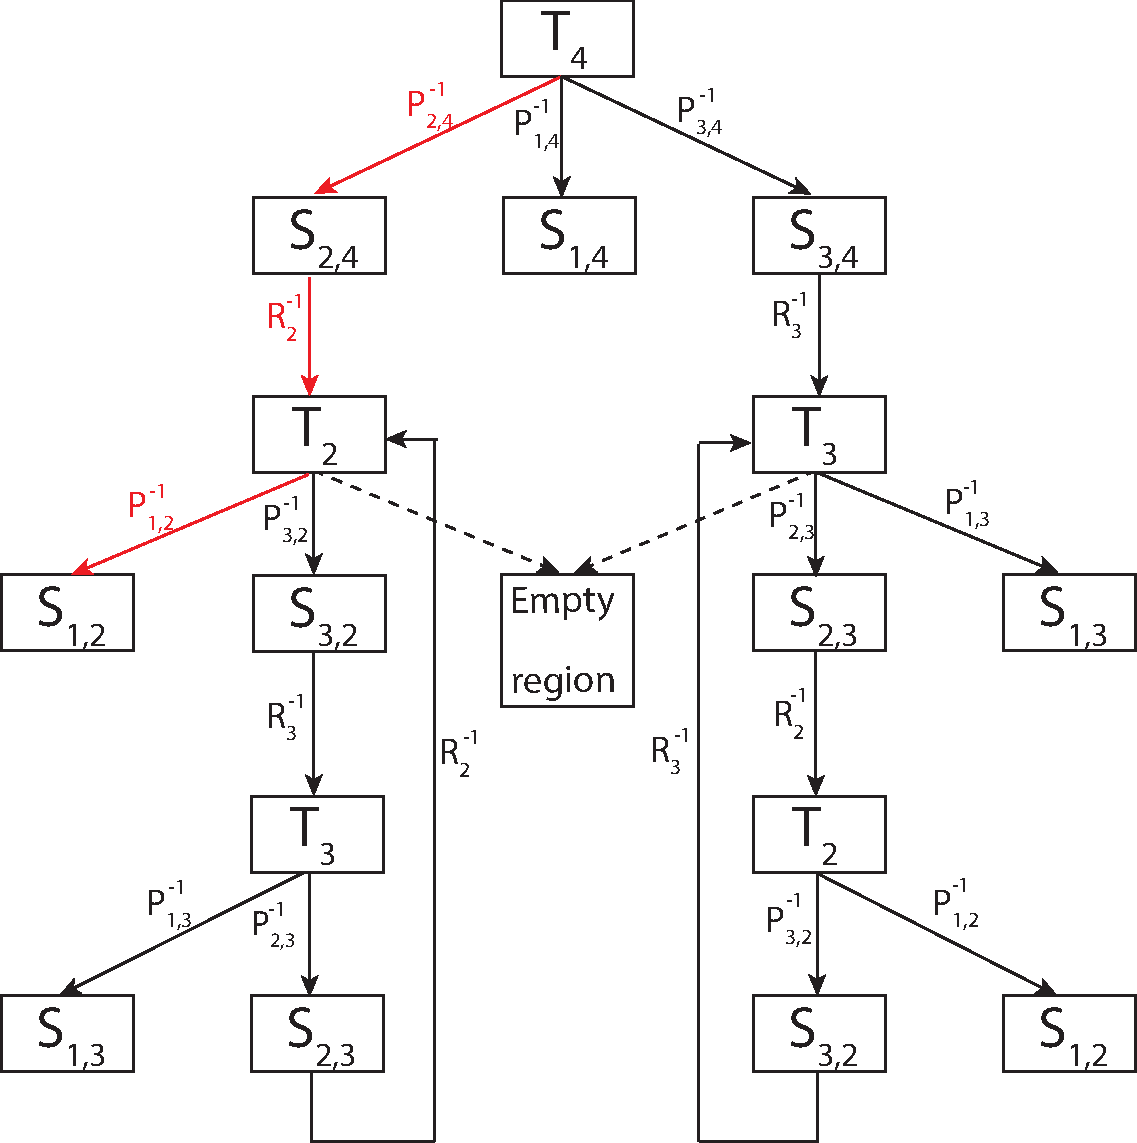
\includegraphics[width = \textwidth]{tree2}
\label{fig:tree}
  \end{center}
\caption{Tree that describes how to detect all the possible paths from \point{S} to \point{T}.}
\label{fig:tree}
\end{figure}
%%\newpage
\\ \indent Using the procedure explained above, given a ray with coordinates
$(\variabile{q}, \variabile{p})\in \mbox{\set{T}{$4$}{}}$ we can establish whether it is located inside one of the regions $\mbox{\set{R}{}{}}(\Pi)$ with positive luminance or not.
In case the ray is inside a region $\mbox{\set{R}{}{}}(\Pi)$,
its corresponding coordinates $(\pos{s,}{$1$},\dir{s,}{$1$})\in \mbox{\set{S}{$1$}{}}$ are obtained using $\inversemap{M}{1,}{4}(\Pi)$, where $\Pi$ is the path followed by this ray. The luminance in Equation ($\ref{LT4}$) is, therefore, defined as in Equation (\ref{eq:PSluminance}), 
for some path $\Pi$ connecting \point{S}{}{} and \point{T}{}{}.
Assuming a Lambertian source and employing conservation of luminance along a ray (see \cite{chaves2015introduction}, Chapter 16), we have that $L$
is a positive constant inside \set{R}{}{}($\Pi$) and it has no contribution on the other parts of \set{T}{$4$}{}.
Indicating with $\variabile{q}^\textrm{\,min}(\Pi,\variabile{p})$ and $\variabile{q}^\textrm{\,max}(\Pi,\variabile{p})$ the minimum and maximum position coordinates of the intersection points between the boundaries $ \partial$\set{R}{}{}($\Pi$) and line $\variabile{p}= \mbox{const}$,
Eq. (\ref{I(eta)}) reduces to Equation (\ref{eta2}), if only two intersection points are found, and to Equation (\ref{eq:Ips}) in case more than two intersection points occur. For the two-faceted cup there are only two intersection points between line $\dir{}{}{}=const$ and $\partial$\set{R}{}{}$(\Pi)$, hence, in this chapter we use Equation (\ref{eta2}) for the intensity calculation.
We remark that, for a given ray with corresponding coordinates $(\pos{}{}, \dir{}{})$ on \set{T}{$4$}{}, only one path is possible as we are assuming that all lines are reflective lines.
Because of this, the regions \set{R}{}{}($\Pi$) do not overlap.
where the intersection is over all the possible paths. 
Next, the details of the procedure to compute the coordinates $\variabile{q}^\textrm{\,min}(\Pi, \variabile{p})$ and $\variabile{q}^\textrm{\,max}(\Pi, \variabile{p})$
are explained. \\ \indent
The goal is to determine the intensity of the light that reaches the target with a given direction $\variabile{p}=\const{const}$.
Since we assume a Lambertian source, this is equal to the sum of the lengths of the line segments given by the intersection of the line $\variabile{p} = \mbox{const}$ and the support of $L$ (see Eq. (\ref{eta2})).
To determine these line segments, a recursive procedure is developed.
The procedure starts on \set{T}{$4$}{} with a given direction $\variabile{p} = \const{const.}$ and with the parallel rays corresponding to the end points $(\pos{}{}^{\textrm{min}}, \variabile{p}) = (-\variabile{b}, \variabile{p})$ and $(\pos{}{}^{\textrm{max}}, \variabile{p}) = (\variabile{b}, \variabile{p})$. 
We set the initial intensity $I(\variabile{p})=0$ along direction $\variabile{p} = \const{const.}$. 
Considering the intersection between the line $\variabile{p}=\textrm{const}$ and the boundaries ($\partial$\set{T}{$4$,}{i})$_{\lineai=1,2,3}$ three intervals are found.
Each interval corresponds to rays emitted by line $\variabile{i}$ (\variabile{i}$=\{1,2,3\}$).
The rays corresponding to the end points of these intervals are traced back from \set{T}{$4$}{} to \set{T}{\lineai}{} where $\lineai$ is the line from which
the rays are emitted. Then, another interval of parallel rays along the corresponding direction in \set{T}{\lineai}{} has to be considered and the intersection points between the line $\dir{}{} = \dir{t,}{\lineai}$ and $\partial$\set{T}{\lineai,}{\lineaj} (with $\variabile{j}\neq\lineai,4$) are calculated, where $\dir{t,}{\lineai}$ is the new direction of the rays traced back.
The procedure continues recursively until the source is found. 
\\ \indent Before explaining the details, let us introduce some notation. The role of the variables we introduce will become clear later on in this chapter.
The coordinates in \set{T}{\lineaj}{} of the rays traced back from line $\lineai\neq\lineaj$ to
line $\lineaj$ are indicated with $(\pos{t,}{\lineaj}^1, \dir{t,}{\lineaj})$ and $(\pos{t,}{\lineaj}^2, \dir{t,}{\lineaj})$.
The minimum and the maximum position coordinates are $\pos{t,}{\lineaj}^\textrm{\,min} = \min\{\pos{t,}{\lineaj}^1, \pos{t,}{\lineaj}^2\}$ and 
$\pos{t,}{\lineaj}^\textrm{\,max} = \max\{\pos{t,}{\lineaj}^1, \pos{t,}{\lineaj}^2\}$, respectively. The coordinates of the intersection points of
$\variabile{p}= \dir{t,}{\lineaj}$ with boundaries $\partial$\set{T}{\lineaj,}{\lineai} need to be determined for every $\lineai = \{1,2,3\}$ and $\lineaj = \{2,3,4\}$ with $\lineaj\neq\lineai$. 
They are indicated with  $(\variabile{u}_{\lineaj,\lineai}^\textrm{\,min}, \dir{t,}{\lineaj})$ and $(\variabile{u}_{\lineaj,\lineai}^\textrm{\,max}, \dir{t,}{\lineaj})$ where 
$\variabile{u}_{\lineaj,\lineai}^\textrm{\,min}<\variabile{u}_{\lineaj,\lineai}^\textrm{\,max}$. 
Since not all the rays whose corresponding coordinates are located inside the segment
$[\pos{t,}{\lineaj}^\textrm{\,min}, \pos{t,}{\lineaj}^\textrm{\,max}]$ with direction $ \dir{}{} =\dir{t,}{\lineaj}$ follow the same path, the intersection segment 
$[\variabile{v}_{\lineaj,\lineai}^\textrm{\,min}, \variabile{v}_{\lineaj,\lineai}^\textrm{\,max}] = [\pos{t,}{\lineaj}^\textrm{\,min}, \pos{t,}{\lineaj}^\textrm{\,max}] \cap [\variabile{u}_{\lineaj,\lineai}^\textrm{\,min}, \variabile{u}_{\lineaj,\lineai}^\textrm{\,max}]$ needs to be calculated. $(\variabile{v}_{\lineaj,\lineai}^\textrm{\,min},\dir{t,}{\lineaj})$ and $(\variabile{v}_{\lineaj,\lineai}^\textrm{\,max},\dir{t,}{\lineaj})$ are the coordinates of the rays that need to be traced back from line $\lineaj$ to line $\lineai$.
\\ \indent The method can be outlined as follows.
\begin{enumerate}
\item Calculate the intersection points $(\variabile{u}_{4,\lineai}^\textrm{\,min}, \variabile{p})$ and $(\variabile{u}_{4,\lineai}^\textrm{\,max}, \variabile{p})$ between line $\variabile{p}= \const{const.}$ and $\partial$\set{T}{$4$,}{\lineai} for every $\lineai=\{1,2,3\}$, where $\variabile{u}_{4,\lineai}^\textrm{\,min}<\variabile{u}_{4,\lineai}^\textrm{\,max}$. This can be done analytically because the exact expression of the boundaries $\partial$\set{T}{$4$,}{\lineaj} is found as explained in the previous paragraph.
\item Calculate the intersection segment 
\begin{equation*}
[\variabile{v}_{4, \lineai}^\textrm{\,min}, \variabile{v}_{4, \lineai}^\textrm{\,max}] = [\variabile{u}_{4, \lineai}^\textrm{\,min}, \variabile{u}_{4, \lineai}^\textrm{\,max}]\cap
 [\pos{}{}^\textrm{\,min}, \pos{}{}^\textrm{\,max}]
\end{equation*}
\item If $\lineai= 1$, coordinates $(\variabile{v}_{4,1}^\textrm{\,min}, \variabile{p})$ and $(\variabile{v}_{4,1}^\textrm{\,max}, \variabile{p})$ equal the coordinates $(\variabile{q}^\textrm{\,min}(\Pi, \variabile{p}), \variabile{p})$ and $(\variabile{q}^\textrm{\,max}(\Pi, \variabile{p}), \variabile{p})$ of the rays located on the boundary $\partial$\set{R}{}{}$(\Pi)$ with $\Pi = (1,4)$. All the parallel rays with direction coordinate $\variabile{p}$ and $\variabile{q}$-position coordinate $\variabile{u}_{4,1}^\textrm{\,min}\leq \variabile{q} \leq \variabile{u}_{4,1}^\textrm{\,max}$ are emitted by the source and they directly hit the target. \\
\indent Update the intensity using Eq. (\ref{eta2})
\begin{equation*}
I(\variabile{p})= I(\variabile{p})+\variabile{q}^\textrm{\,min}(\Pi, \dir{}{})-\variabile{q}^\textrm{\,max}(\Pi, \dir{}{}).
\end{equation*}
\item If $\lineai\neq 1$, continue with the following steps
\item Trace back $(\variabile{v}_{4,\lineai}^\textrm{\,min}, \variabile{p})$ and $(\variabile{v}_{4,\lineai}^\textrm{\,max}, \variabile{p})$ from line $4$ to line $\lineai$ to find their corresponding coordinates on \set{T}{\lineai}{}
\begin{equation*}
\begin{aligned}
(\pos{t,}{\lineai}^{\,1}, \dir{t,}{\lineai})& =\inversemap{R}{\lineai}{}\circ \inversemap{P}{\lineai,}{4}(\variabile{v}_{4,\lineai}^\textrm{\,min}, \variabile{p})  \\
(\pos{t,}{\lineai}^{\,2}, \dir{t,}{\lineai}) & =\inversemap{R}{\lineai}{}\circ \inversemap{P}{\lineai,}{4}(\variabile{u}_{4,\lineai}^\textrm{\,max}, \variabile{p})
\end{aligned}
\end{equation*}
\item Update the path $\Pi = (\lineai, 4)$
\item Determine $\pos{t,}{\lineai}^\textrm{\,min}= \min\{\pos{t,}{\lineai}^{\,1}, \pos{t,}{\lineai}^{\,2}\}$ and $\pos{t,}{\lineai}^\textrm{\,max}= \max\{\pos{t,}{\lineai}^{\,1}, \pos{t,}{\lineai}^{\,2}\}$
\item Calculate the intersection points $(\variabile{u}_{\lineai,\lineaj}^\textrm{\,min}, \variabile{p})$ and $(\variabile{u}_{\lineai,\lineaj}^\textrm{\,max}, \variabile{p})$ between line $\dir{t,}{\lineai}$ and 
$\partial$\set{T}{\lineai,}{\lineaj} for every $\lineaj=\{1,2,3\}$ with $\lineaj\neq\lineai$.
\item Since not all rays whose corresponding coordinates are located inside the segment
$[\pos{t,}{\lineai}^\textrm{\,min}, \pos{t,}{\lineai}^\textrm{\,max}]$ follow the same path,
 compute the intersection segment 
\begin{equation*}
[\variabile{v}_{\lineai, \lineaj}^\textrm{\,min}, \variabile{v}_{\lineai, \lineaj}^\textrm{\,max}] = [\variabile{u}_{\lineai, \lineaj}^\textrm{\,min}, \variabile{u}_{\lineai, \lineaj}^\textrm{\,max}]\cap
 [\pos{t,}{\lineai}^\textrm{\,min}, \pos{t,}{\lineai}^\textrm{\,max}].
\end{equation*}
\item For $\lineaj\neq 1$ 
\begin{itemize}
\item[a)] Trace back $(\variabile{v}_{\lineai, \lineaj}^\textrm{\,min}, \dir{t,}{\lineai})$ and $(\variabile{v}_{\lineai, \lineaj}^\textrm{\,max}, \dir{t,}{\lineai})$ from $\lineai$ to $\lineaj$ 
\begin{equation*}
\begin{aligned}
(\pos{t,}{\lineaj}^{\,1}, \dir{t,}{\lineaj})& =\inversemap{R}{\lineaj}{}\circ \inversemap{P}{\lineaj,}{\lineai}(\variabile{v}_{\lineai, \lineaj}^\textrm{\,min}, \dir{t,}{\lineai}),  \\
(\pos{t,}{\lineaj}^{\,2}, \dir{t,}{\lineaj}) & =\inversemap{R}{\lineaj}{}\circ \inversemap{P}{\lineaj,}{\lineai}(\variabile{v}_{\lineai, \lineaj}^\textrm{\,max}, \dir{t,}{\lineai}).
\end{aligned}
\end{equation*}
\item[b)] Update the path $\Pi = (\lineaj, \Pi)$
\item[c)] Put $\lineai=\lineaj$ and repeat the procedure from point $7$.
\end{itemize}
\item If $\lineaj=1$, the rays reached the source and a possible path $\Pi = (1, \cdots, 4)$ is found. 
\begin{itemize}
\item[a)]
Apply 
\begin{equation*}
\begin{aligned}
(\pos{s,}{$1$}^{\,1}, \dir{s,}{$1$})& = \inversemap{P}{1,}{\lineai}(\variabile{v}_{\lineai, 1}^\textrm{\,min}, \dir{t,}{\lineai})  \\
(\pos{s,}{$1$}^{\,2}, \dir{s,}{$1$}) & =\inversemap{P}{1,}{\lineai}(\variabile{v}_{\lineai, 1}^\textrm{\,max}, \dir{t,}{\lineai})
\end{aligned}
\end{equation*}
\item[b)] Apply the direct map $\mapnumb{M}_{1,4}(\Pi)$ restricted to the path $\Pi$ found:
\begin{equation*}
\begin{aligned}
 (\pos{}{}^{1}(\Pi, \dir{}{}), \dir{}{})&= \mapnumb{M}_{1,4}(\Pi)(\pos{s,}{$1$}^{\,1}, \dir{s,}{$1$})\\
 (\pos{}{}^{2}(\Pi, \dir{}{}), \dir{}{})&= \mapnumb{M}_{1,4}(\Pi)(\pos{s,}{$1$}^{\,2}, \dir{s,}{$1$})
\end{aligned}
\end{equation*}
\item[c)] Update intensity $$I(\variabile{p}) = I(\variabile{p})+\pos{}{}^{\textrm{min}}(\Pi, \dir{}{})- \pos{}{}^{\textrm{max}}(\Pi, \dir{}{})$$
where $\pos{}{}^\textrm{min} = \min\{ \pos{}{}^{1}(\Pi, \dir{}{}), \pos{}{}^{2}(\Pi, \dir{}{})\}$ and $\pos{}{}^\textrm{max} = \max\{\pos{}{}^{1}(\Pi, \dir{}{}), \pos{}{}^{2}(\Pi, \dir{}{})\}.$
\end{itemize}
\end{enumerate}
\indent
To clarify the technique, we make an example that describes how the target intensity along direction $\variabile{p}= -0.2$ is calculated.
From Fig. $\ref{fig:T41}$ to Fig. $\ref{fig:T43}$ the steps used in this example are shown.
A detailed description of those figures is given in the following.
\\ \indent The procedure starts with the rays with direction $\variabile{p} = 0.2$ on \set{T}{$4$}{}, where $\variabile{q}^\textrm{min}= -\variabile{b}$ and
$\variabile{q}^\textrm{max}= \variabile{b}$ are the left and the right end points of the target \point{T}, respectively.
 The intersection points $(\variabile{u}_{4,\lineai}^\textrm{\,min}, \variabile{p})$ and
$(\variabile{u}_{4,\lineai}^\textrm{\,max}, \variabile{p})$
of the line $\variabile{p}= -0.2$
 with boundaries $\partial\mbox{\set{T}{$4$,}{\lineai}}$ are computed for every $\lineai\neq 4$. \\ \indent
We start from $\lineai=1$. Therefore the coordinates  $(\variabile{u}_{4,1}^\textrm{\,min}, \variabile{p})$ and
$(\variabile{u}_{4,1}^\textrm{max}, \variabile{p})$ of the intersection points between line $\variabile{p} = -0.2$ and the boundary $\partial\mbox{\set{T}{$4$,}{$1$}}$ are computed and these points are depicted in Fig. \ref{fig:T41}.
 The source is now reached because $\lineai = 1$ and, one possible path is found.
 The points $(\variabile{u}_{4,1}^\textrm{\,min}, \variabile{p})$
and $(\variabile{u}_{4,1}^\textrm{\,max}, \variabile{p})$ are located on the boundaries of the region formed by the rays that leave the source and directly hit the target, that is the rays located on
$\partial \mbox{\set{R}{}{}}(\Pi_1)$ with $\Pi_1 = (1,4)$.
Therefore, the contribution to the intensity formed by the rays that follow the path $\Pi_1 = (1,4)$ is given by 
$\variabile{u}_{4,1}^\textrm{\,max}-\variabile{u}_{4,1}^\textrm{\,min}$. \\ \indent
We continue with $\lineai = 2$. 
The boundary $\partial\mbox{\set{T}{$4$,}{$2$}}$ is considered in order to find other paths.
The intersection points $(\variabile{u}_{4,2}^\textrm{\,min}, \variabile{p})$ and
$(\variabile{u}_{4,2}^\textrm{\,max}, \variabile{p})$ of line
$\variabile{p}=-0.2$ with the boundary
$\partial\mbox{\set{T}{$4$,}{$2$}}$ are calculated.
They are depicted in Fig. \ref{fig:T42} with the magenta dots. also the intersection segment 
\begin{equation}
[\variabile{v}_{4,2}^\textrm{\,min}, \variabile{v}_{4,2}^\textrm{\,max}] = [\variabile{u}_{4,2}^\textrm{\,min}, \variabile{u}_{4,2}^\textrm{\,max}]\cap [\variabile{q}^\textrm{min}, \variabile{q}^\textrm{max}]
\end{equation}
is calculated\footnote{In \set{T}{$4$}{} $\variabile{v}_{4,2}^\textrm{\,min} = \variabile{u}_{4,2}^\textrm{\,min}$ and $\variabile{v}_{4,2}^\textrm{\,max} = \variabile{u}_{4,2}^\textrm{\,max}$ because $\variabile{q}^\textrm{min} = -\variabile{b}$ and $\variabile{q}^\textrm{max} = \variabile{b}$ always coincide with the end points of \set{T}{$4$}{}.}.
Their corresponding position coordinates $\pos{s,}{$2$}^1$ and $\pos{s,}{$2$}^2$ on \set{S}{$2$}{}
are obtained from:
\begin{equation}\label{inverseP}
\begin{split}
 \inversemap{P}{2,}{4}
(\variabile{v}_{4,2}^\textrm{\,min}, \variabile{p}) &=  (\pos{s,}{$2$}^1, \dir{s,}{2}), \\
 \inversemap{P}{2,}{4}
(\variabile{v}_{4,2}^\textrm{\,max}, \variabile{p}) &=  (\pos{s,}{$2$}^2, \dir{s,}{2}).
\end{split}
\end{equation}
 The directions
$\dir{s,}{$2$}^\textrm{\,min}$ and $\dir{s,}{$2$}^\textrm{\,max} $ on \set{S}{$2$}{}
are given considering the direction $\dir{t,}{$2$} = \dir{}{}$ with respect to the normal
$\boldsymbol{\nu}_{2}$ of line $2$.
 Note that $\dir{s,}{$2$}^1=\dir{s,}{$2$}^2$ because all the lines are straight, their normals do not depend on the position at which it is computed.
 Then, the corresponding direction $\dir{t,}{$2$}^1=\dir{t,}{$2$}^2$ on \set{T}{$2$}{}
 is calculated from:
\begin{equation}\label{inverseR}
\begin{split}
\inversemap{R}{2}{}(\pos{s,}{$2$}^1, \dir{s,}{$2$}) &= (\pos{t,}{$2$}^1, \dir{t,}{$2$}), \\
\inversemap{R}{2}{}(\pos{s,}{$2$}^2, \dir{s,}{$2$}) &= (\pos{t,}{$2$}^2, \dir{t,}{$2$}).
\end{split}
\end{equation}
Note that $\pos{s,}{$2$}^1 = \pos{t,}{$2$}^1$ and $\pos{s,}{$2$}^2= \pos{t,}{$2$}^2$ since the reflection map does not change the position coordinates.
 Eqs. (\ref{inverseP}) and (\ref{inverseR}) lead to: \begin{equation}
\begin{split}
\inversemap{R}{2}{}\circ \inversemap{P}{2,}{4}(\variabile{v}_{4,2}^\textrm{\,min}, \variabile{p}) &= (\pos{t,}{$2$}^1, \dir{t,}{$2$}),\\
\inversemap{R}{2}{}\circ \inversemap{P}{2,}{4}(\variabile{v}_{24,}^\textrm{\,max}, \variabile{p}) &= (\pos{t,}{$2$}^2, \dir{t,}{$2$}).
\end{split}
\end{equation} The map $\inversemap{R}{2}{}\circ \inversemap{P}{2,}{4}$  is depicted in red in Fig. \ref{fig:tree}.
The minimum 
 $\pos{t,}{$2$}^\textrm{\,min} = \min\{\pos{t,}{$2$}^1, \pos{t,}{$2$}^2\}$ and the maximum
 $\pos{t,}{$2$}^\textrm{\,max} = \max\{\pos{t,}{$2$}^1, \pos{t,}{$2$}^2\}$ are calculated. The points with coordinates  $(\pos{t,}{$2$}^\textrm{\,min}, \dir{t,}{$2$})$  and  $(\pos{t,}{$2$}^\textrm{\,max}, \dir{t,}{$2$})$  are depicted in Fig. \ref{fig:T21} where $\dir{t,}{$2$}=0.82$.
 To understand whether the corresponding rays are illuminated or not by the source, the preceding procedure used for
 \set{T}{$4$}{} is now applied to \set{T}{$2$}{}
 along direction $\dir{t,}{$2$}=0.82$. \\ \indent
  Next, the intersection points $(\variabile{u}_{2,\lineai}^\textrm{\,min}, \dir{t,}{$2$})$ and
$(\variabile{u}_{2,\lineai}^\textrm{\,max}, \dir{t,}{$2$})$
of line $\dir{t,}{$2$}= 0.82$
 with boundaries $\partial\mbox{\set{T}{$2$,}{\lineai}}$ are computed for every $\lineai\in\{1,3\}.$
 We start from the boundary $\partial$\set{T}{$2$,}{$1$} obtaining the points $(\variabile{u}_{2, 1}^\textrm{\,min}, \dir{t,}{$2$})$ and
 $(\variabile{u}_{2, 1}^\textrm{\,max}, \dir{t,}{$2$})$ shown in Fig. \ref{fig:T21}.
 Now, the position coordinates $\variabile{v}_{2, 1}^\textrm{\,min} = \max\{\pos{t,}{$2$}^ \textrm{\,min},\variabile{u}_{2,1}^\textrm{\,min}\}$
 and $\variabile{v}_{2, 1}^\textrm{\,max} = \min\{\pos{t,}{$2$}^ \textrm{\,max},\variabile{u}_{2, 1}^\textrm{\,max}\}$ need to be considered.
 All the rays located inside the segment $[\variabile{v}_{2, 1}^\textrm{\,min},\variabile{v}_{2, 1}^\textrm{\,max}]$ in
  \set{T}{$2$}{} and with direction $\dir{t,}{2}$ follow the path $\Pi_2 = (1,2,4)$. In particular, the rays corresponding to the coordinates $(\variabile{v}_{2, 1}^\textrm{\,min},\dir{t,}{2} )$ and $(\variabile{v}_{2, 1}^\textrm{\,max},\dir{t,}{2} )$ are  located on the boundaries of the region \set{R}{}{}$(\Pi_2)$ on \set{T}{$4$}{}
  formed by all the rays that follow path $\Pi_2$.
  Their corresponding coordinates $(\variabile{q}^{1}(\Pi_2, \variabile{p}), \variabile{p})$ and
 $(\variabile{q}^{2}(\Pi_2, \variabile{p}), \variabile{p})$ on \set{T}{$4$}{} are obtained from:\footnote{With a slight abuse of notation we indicate  $\variabile{q}^{1}(\Pi, \variabile{p})$ with $\variabile{q}^{1}$ and 
$ \variabile{q}^{2}(\Pi, \variabile{p})$ with $\variabile{q}^{2}$.}
\begin{equation}
\begin{split}
\mapnumb{P}_{2,4} \circ \mapnumb{R}_{2} (\variabile{v}_{2, 1}^\textrm{\,min},\dir{t,}{$2$} ) & = (\variabile{q}^{1}, \variabile{p}), \\
\mapnumb{P}_{2,4} \circ \mapnumb{R}_{2} (\variabile{v}_{2, 1}^\textrm{\,max},\dir{t,}{$2$} ) & = (\variabile{q}^{2}, \variabile{p}).
\end{split}
\end{equation} 
The rays corresponding to the coordinates  $(\variabile{q}^{1}, \variabile{p})$ and $ (\variabile{q}^{1}, \variabile{p})$ are located
 on the boundary $\partial$\set{R}{}{}$(\Pi_2)$ along direction $\variabile{p}=-0.2$.
Indicating with $\variabile{q}^{\textrm{min}} = \min\{\variabile{q}^{1}, \variabile{q}^2\}$ and $\variabile{q}^{\textrm{max}} = \max\{\variabile{q}^{1}, \variabile{q}^2\}$, the distance $\variabile{q}^{\textrm{max}}-\variabile{q}^{\textrm{min}}$ gives the contribution to the intensity $I(\variabile{p})$ of the rays located in \set{R}{}{}$(\Pi_2)$ where $\variabile{p}=-0.2$.\\
\indent  \set{T}{$2$}{} can also be illuminated by line $3$, therefore the intersection points $(\variabile{u}_{2, 3}^\textrm{\,min}, \dir{t,}{$2$})$ and $(\variabile{u}_{2, 3}^\textrm{\,max}, \dir{t,}{$2$})$ of line
 $\dir{t,}{$2$}=0.82$ and $\partial \mbox{\set{T}{$2$,}{$3$}}$ are calculated, these points are depicted in Fig. \ref{fig:T22}.
 The coordinates $(\variabile{v}_{2, 3}^\textrm{\,min}, \dir{t,}{$2$})$ and $(\variabile{v}_{2, 3}^\textrm{\,max}, \dir{t,}{$2$})$ are shown in the same figure.
 As the source is not reached yet ($\lineai=3$), the rays corresponding to $(\variabile{v}_{2, 3}^\textrm{\,min}, \dir{t,}{$2$})$ and $(\variabile{v}_{2, 3}^\textrm{\,max}, \dir{t,}{$2$})$ are followed back using the inverses of the propagation and the reflection maps. The coordinates on \set{T}{$3$}{} are shown in Fig. \ref{fig:T31} with blue circles and they obtained from:
 \begin{equation}
\begin{split}
\inversemap{R}{3}{}\circ \inversemap{P}{2,3}(\variabile{v}_{2, 3}^\textrm{\,min}, \dir{t,}{$2$}) &= (\pos{t,}{$3$}^{1}, \dir{t,}{$3$}),\\
\inversemap{R}{3}{}\circ \inversemap{P}{2,3}(\variabile{v}_{2, 3}^\textrm{\,max}, \dir{t,}{$2$}) &= (\pos{t,}{$3$}^{2}, \dir{t,}{$3$}).
\end{split}
\end{equation}
The minimum and the maximum position coordinates are $\pos{t,}{$3$}^{\textrm{min}}= \min\{\pos{t,}{$3$}^{1}, \pos{t,}{$3$}^{2}\}$ and 
$\pos{t,}{$3$}^{\textrm{max}}= \max\{\pos{t,}{$3$}^{1}, \pos{t,}{$3$}^{2}\}$, respectively.
We found that $\variabile{v}_{3,2}^\textrm{max}\neq\variabile{u}_{3,2}^\textrm{max}$ because $[\pos{t,}{$3$}^\textrm{min}, \pos{t,}{$3$}^\textrm{max}]\subset
[\variabile{u}_{3,2}^\textrm{min},\variabile{u}_{3,2}^\textrm{max}]$, this means that the rays with corresponding position coordinates inside the interval 
$[\pos{t,}{$3$}^\textrm{max},\variabile{u}_{3,2}^\textrm{max}]$ will follow a different path. 
The procedure continues recursively.
  It stops either when the rays encounter the source, i.e. when $\lineai=1$, or when no intersection points between the
  direction $\variabile{p}=\dir{t,}{\lineaj}$ and the boundaries $\partial$\set{T}{\lineaj,}{\lineai} are found for any $\lineai={1,2,3}$ with $\lineai\neq\lineaj$. \\ \indent
  If the source is reached, then a valid path $\Pi = (1,3,2,4)$ is found. Using the inverse of the propagation map, we compute
\begin{equation}
\begin{aligned}
\inversemap{P}{1,3}(\pos{t,}{$3$}^\textrm{min}, \dir{t,}{$3$}) = (\pos{s,}{$1$}^1, \dir{s,}{$1$}), \\ 
\inversemap{P}{1,3}(\pos{t,}{$3$}^\textrm{max}, \dir{t,}{$3$}) = (\pos{s,}{$1$}^2, \dir{s,}{$1$}).
 \end{aligned}
\end{equation} 
The direct map $\mapnumb{M}_{1,4}(\Pi)$:\set{S}{$1$}{}$\mapsto$\set{R}{}{}$(\Pi)$ restricted to path $\Pi = (1,3,2,4)$, i.e.
\begin{equation}
\mapnumb{M}_{1,4} = \mapnumb{P}_{2,4}\circ\mapnumb{R}_{2}\circ\mapnumb{P}_{3,2}\circ\mapnumb{R}_{3}\circ\mapnumb{P}_{1,3}
\end{equation}
is applied to the coordinates $(\pos{s,}{$1$}^{1}, \dir{s,}{$1$})$ and $(\pos{s,}{$1$}^{1}, \dir{s,}{$1$})$ giving:
\begin{equation}
\begin{split}
\mapnumb{M}_{1,4}(\pos{s,}{$1$}^{1}, \dir{s,}{$1$}) &= (\variabile{q}^{1}(\Pi, \variabile{p}), \variabile{p}),\\
\mapnumb{M}_{1,4}(\pos{s,}{$1$}^{2}, \dir{s,}{$1$}) &= (\variabile{q}^{2}(\Pi, \variabile{p}), \variabile{p}).
\end{split}
\end{equation} 
the coordinates $(\variabile{q}^{1}(\Pi, \variabile{p}), \variabile{p})$ and
  $(\variabile{q}^{2}(\Pi, \variabile{p}), \variabile{p})$ located on $\partial$\set{R}{}{}$(\Pi)$ in \set{T}{$4$}{} are found.
Indicating with $\variabile{q}^{\textrm{min}}= \min\{\variabile{q}^{1}, \variabile{q}^{2}\}$ and $\variabile{q}^{\textrm{max}}= \max\{\variabile{q}^{1}, \variabile{q}^{2}\}$, 
Thus, the contribution to the intensity due to the rays that follow the path $\Pi$ is given by 
\begin{equation}
I(\variabile{p}) = I(\variabile{p})+\variabile{q}^{\textrm{max}}(\Pi, \variabile{p})-\variabile{q}^{\textrm{min}}(\Pi, \variabile{p}). 
\end{equation}
  If no intersection points are found, then the rays traced are
  not emitted by the source, therefore no contribution to the intensity needs to be added. This is, for instance, the case of rays with
  coordinates $(\variabile{v}_{2, 3}^\textrm{\,min}, 0.82)$ and $(\variabile{v}_{2, 3}^\textrm{\,max}, 0.82)$
  on \set{T}{$2$}{} in Fig. \ref{fig:T22}. Below we explain this case in detail. \\ \indent
  In Fig. \ref{fig:T31}, the coordinates $(\pos{t,}{$3$}^{\textrm{min}}, \dir{t,}{$3$})$ and $(\pos{t,}{$3$}^{\textrm{max}}, \dir{t,}{$3$})$ in \set{T}{$3$}{} with $\dir{t,}{$3$}=-0.29$ are shown.
  They are obtained from:
\begin{equation}
\begin{split}
 \inversemap{R}{3}{}\circ\inversemap{P}{3,}{2}(\variabile{v}_{2, 3}^\textrm{\,min}, 0.82)& = (\pos{t,}{$3$}^{1}, \dir{t,}{$3$}),\\
\inversemap{R}{3}{}\circ\inversemap{P}{3,}{2}(\variabile{v}_{2, 3}^\textrm{\,max}, 0.82)& = (\pos{t,}{$3$}^{2}, \dir{t,}{$3$}).
\end{split}
\end{equation}
 From Fig. \ref{fig:T31} we note that there are no intersection points
   of line $\dir{t,}{$3$}=-0.29$ with $\partial\mbox{\set{T}{$3$,}{$1$}}$.
  So, only the coordinates of the intersections $(\variabile{u}_{3, 2}^\textrm{\,min}, -0.29)$ and $(\variabile{u}_{3, 2}^\textrm{\,max}, -0.29)$ between line $\dir{t,}{$3$}=-0.29$ and  $\partial\mbox{\set{T}{$3$,}{$2$}}$ are calculated.
  Next, the intersection interval 
\begin{equation}
[\variabile{v}_{3, 2}^\textrm{\,min},\variabile{v}_{3, 2}^\textrm{\,max}] = [\variabile{u}_{3, 2}^\textrm{\,min}, \variabile{u}_{3, 2}^\textrm{\,max}] \cap [\pos{t,}{$3$}^{\textrm{min}}, \pos{t,}{$3$}^{\textrm{max}}],
\end{equation} formed by parallel rays with direction $\dir{t,}{$3$} = -0.29$, is considered.
  Using: 
\begin{equation}
\begin{split}
 \inversemap{R}{2}{}\circ\inversemap{P}{2,}{3}(\variabile{v}_{3, 2}^\textrm{\,min},-0.29) & = (\pos{t,}{$2$}^{\textrm{min}}, \dir{t,}{$2$}),\\
 \inversemap{R}{2}{}\circ\inversemap{P}{2,}{3}(\variabile{v}_{3, 2}^\textrm{\,max},-0.29) & = (\pos{t,}{$2$}^{\textrm{max}}, \dir{t,}{$2$}),\\
\end{split}
\end{equation}
  the corresponding coordinates $(\pos{t,}{$2$}^{\textrm{max}}, \dir{t,}{$2$})$ and $(\pos{t,}{$2$}^{\textrm{min}}, \dir{t,}{$2$})$ on \set{T}{$2$}{} are found (Fig. \ref{fig:T23})
  with $\dir{t,}{$2$}=-0.41$.
  Now the procedure is repeated again for \set{T}{2}{} along the direction $\dir{t,}{$2$}=-0.41$.
  No intersection points between line $\dir{t,}{$2$}=-0.41$ and $\partial$\set{T}{$2$,}{$1$} occur.
  Only, the intersection points $(\variabile{u}_{2,3}^\textrm{\,min},\dir{t,}{$2$})$ and $(\variabile{u}_{2,3}^\textrm{\,max},\dir{t,}{$2$})$
  of line $\dir{t,}{$2$}=-0.41$ and $\partial$\set{T}{$2$,}{$3$} are found (see Fig. \ref{fig:T23}).
  The intersection segment 
\begin{equation}
[\variabile{v}_{2,3}^\textrm{\,min},\variabile{v}_{2,3}^\textrm{\,max}] = [\pos{t,}{$2$}^\textrm{\,min},\pos{t,}{$2$}^\textrm{\,max}] \cap  [\pos{t,}{$2$}^\textrm{\,min},\pos{t,}{$2$}^\textrm{\,max}]
\end{equation}
is calculated. 
The coordinates on \set{T}{$3$}{} corresponding to the end points of the intersection interval are found using:
\begin{equation}
\begin{split}
\inversemap{R}{3}{}\circ\inversemap{P}{3,}{2} (\variabile{v}_{2,3}^\textrm{\,min},\dir{t,}{$2$})& = (\pos{t,}{$3$}^\textrm{\,min},\dir{t,}{$3$}),\\
\inversemap{R}{3}{}\circ\inversemap{P}{3,}{2} (\variabile{v}_{2,3}^\textrm{\,max},\dir{t,}{$2$})& = (\pos{t,}{$3$}^\textrm{\,max},\dir{t,}{$3$}),
\end{split}
\end{equation}  where $ \dir{t,}{$3$} = 0.91$ (see Fig. \ref{fig:T32}). \\ \indent
 Considering the PS \set{T}{$3$}{} and the direction $\dir{t,}{$3$}=0.91$, we note that there are no intersection points between line
 $\dir{t,}{$3$}=0.91$ and both $\partial$\set{T}{$3$,}{$1$} and $\partial$\set{T}{$3$,}{$2$}.
 Indeed, the whole segment $[\pos{t,}{$3$}^\textrm{\,min},\pos{t,}{$3$}^\textrm{\,max}]$ is outside both
 \set{T}{$3$,}{$2$} and \set{T}{$3$,}{$1$}. Because of this, all the rays with $\variabile{q}$-coordinates inside the interval
 $[\pos{t,}{$3$}^\textrm{\,min},\pos{t,}{$3$}^\textrm{\,max}]$
and with direction $\variabile{p}= \dir{t,}{3}$ are not illuminated by the source and no new real path is found.
\\ \indent
Finally, the recursive procedure is applied to \set{T}{$4$,}{$3$}.
The first step is depicted in Fig. \ref{fig:T43}.
 We decided not to show all the steps for \set{T}{$4$,}{$3$} as they are similar to those used for \set{T}{$4$,}{$2$} and explained above.
 \\ \indent Finally, to compute the intensity along another direction $\variabile{p}^{\lineak}\in[-1,1]$ on \set{T}{$4$}{},
the procedure explained for $\variabile{p}=-0.2$ is repeated for $\variabile{p}= \variabile{p}^{\lineak}$.
In this way we find all the possible paths $\Pi$ and the regions \set{R}{}{}$(\Pi)$ with positive luminance on \set{T}{$4$}{}.
Furthermore, considering every time the coordinates located on the boundaries of the regions \set{T}{\lineai,}{\lineaj} for every $\lineaj$, also the boundaries $\partial$\set{R}{}{}$(\Pi)$ are determined for a given path $\Pi$ as well as the coordinates $\variabile{q}^\textrm{max}(\Pi,\variabile{p})$ and $\variabile{q}^\textrm{\,min}(\Pi,\variabile{p})$ for every $\variabile{p}\in [-1,1]$.
In Algorithm \ref{alg} they are the main steps to calculate the intensity $I(\variabile{p})$ along a given direction
$\variabile{p} = \variabile{p}^{\lineak}$ in \set{T}{$4$}{}, where for the first step we take $\lineaj=4$.
\begin{figure}
\begin{minipage}[]{.48\textwidth}
\centering
   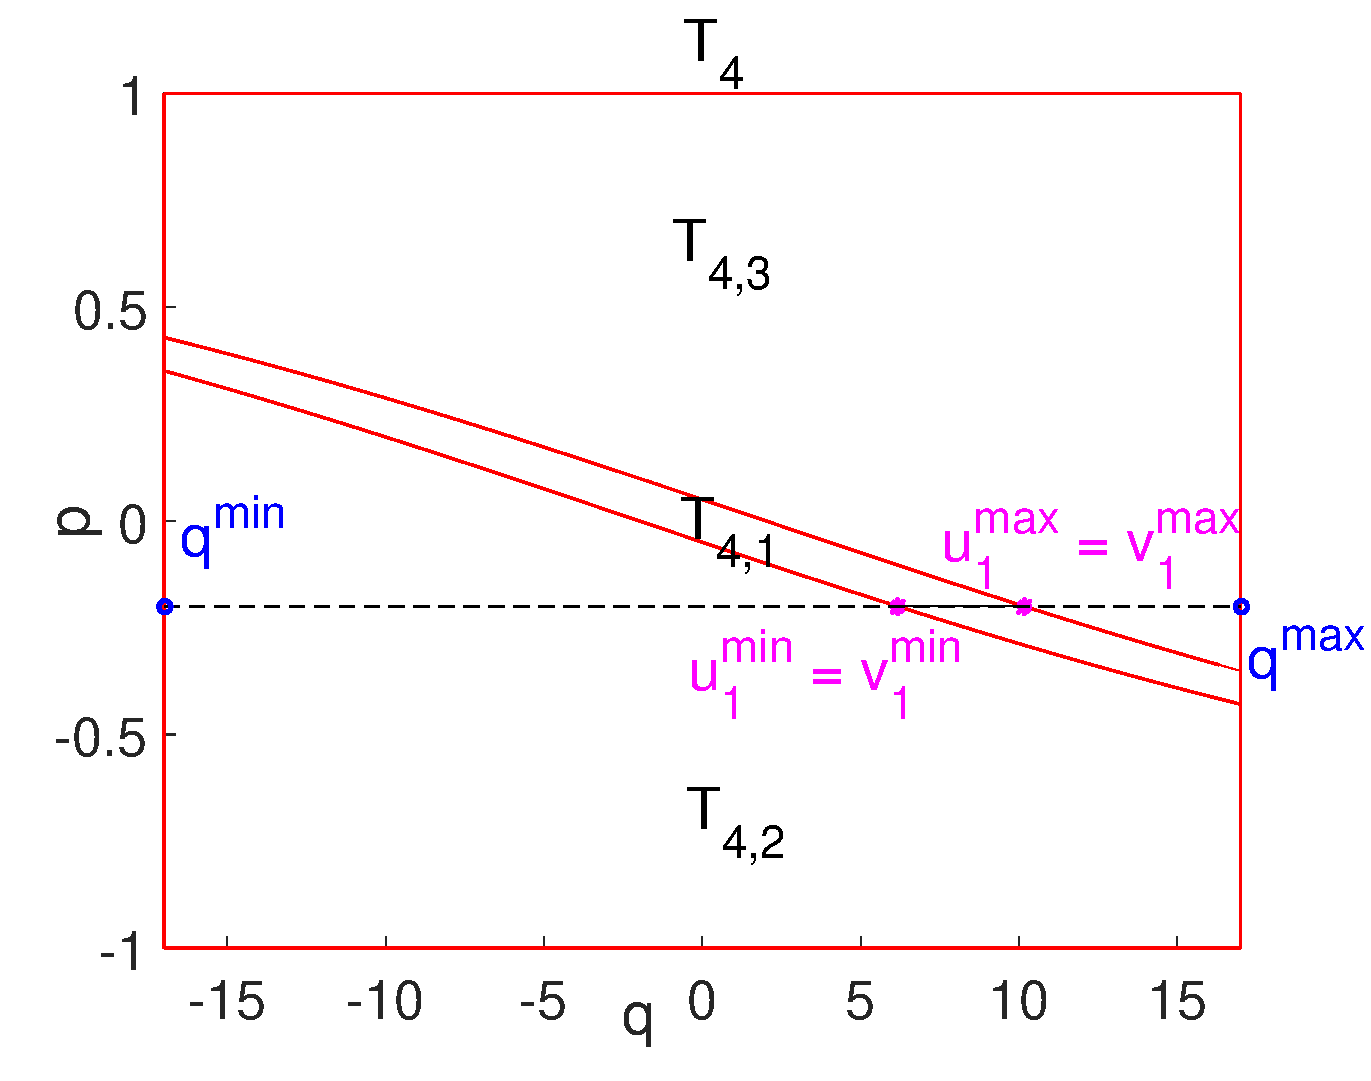
\includegraphics[width=\textwidth]{T4_1}
  \caption{\footnotesize{Target phase space of line $4$. $\pos{t,}{$4$}^{\textrm{min}}$ and $\pos{t,}{$4$}^{\textrm{max}}$ are the $\variabile{x}$-coordinates of the end points of line $4$.
  The intersection points between the line $\variabile{p} = -0.2$ and $\partial$\set{T}{$4$,}{$1$} are $(\variabile{u}_{4,1}^{\textrm{min}}, \variabile{p})$ and
  $(\variabile{u}_{4,1}^{\textrm{max}}, \variabile{p})$. $\variabile{v}_{4,1}^{\textrm{min}}= \max \{\pos{t,}{$4$}^{\textrm{min}}, \variabile{u}_{4,1}^{\textrm{min}}\}$ and
  $\variabile{v}_{4,1}^{\textrm{max}}= \min \{\pos{t,}{$4$}^{\textrm{max}}, \variabile{u}_{4,1}^{\textrm{max}}\}$.}}
   \label{fig:T41}
\end{minipage}
 \begin{minipage}[]{.48\textwidth}
  \centering
   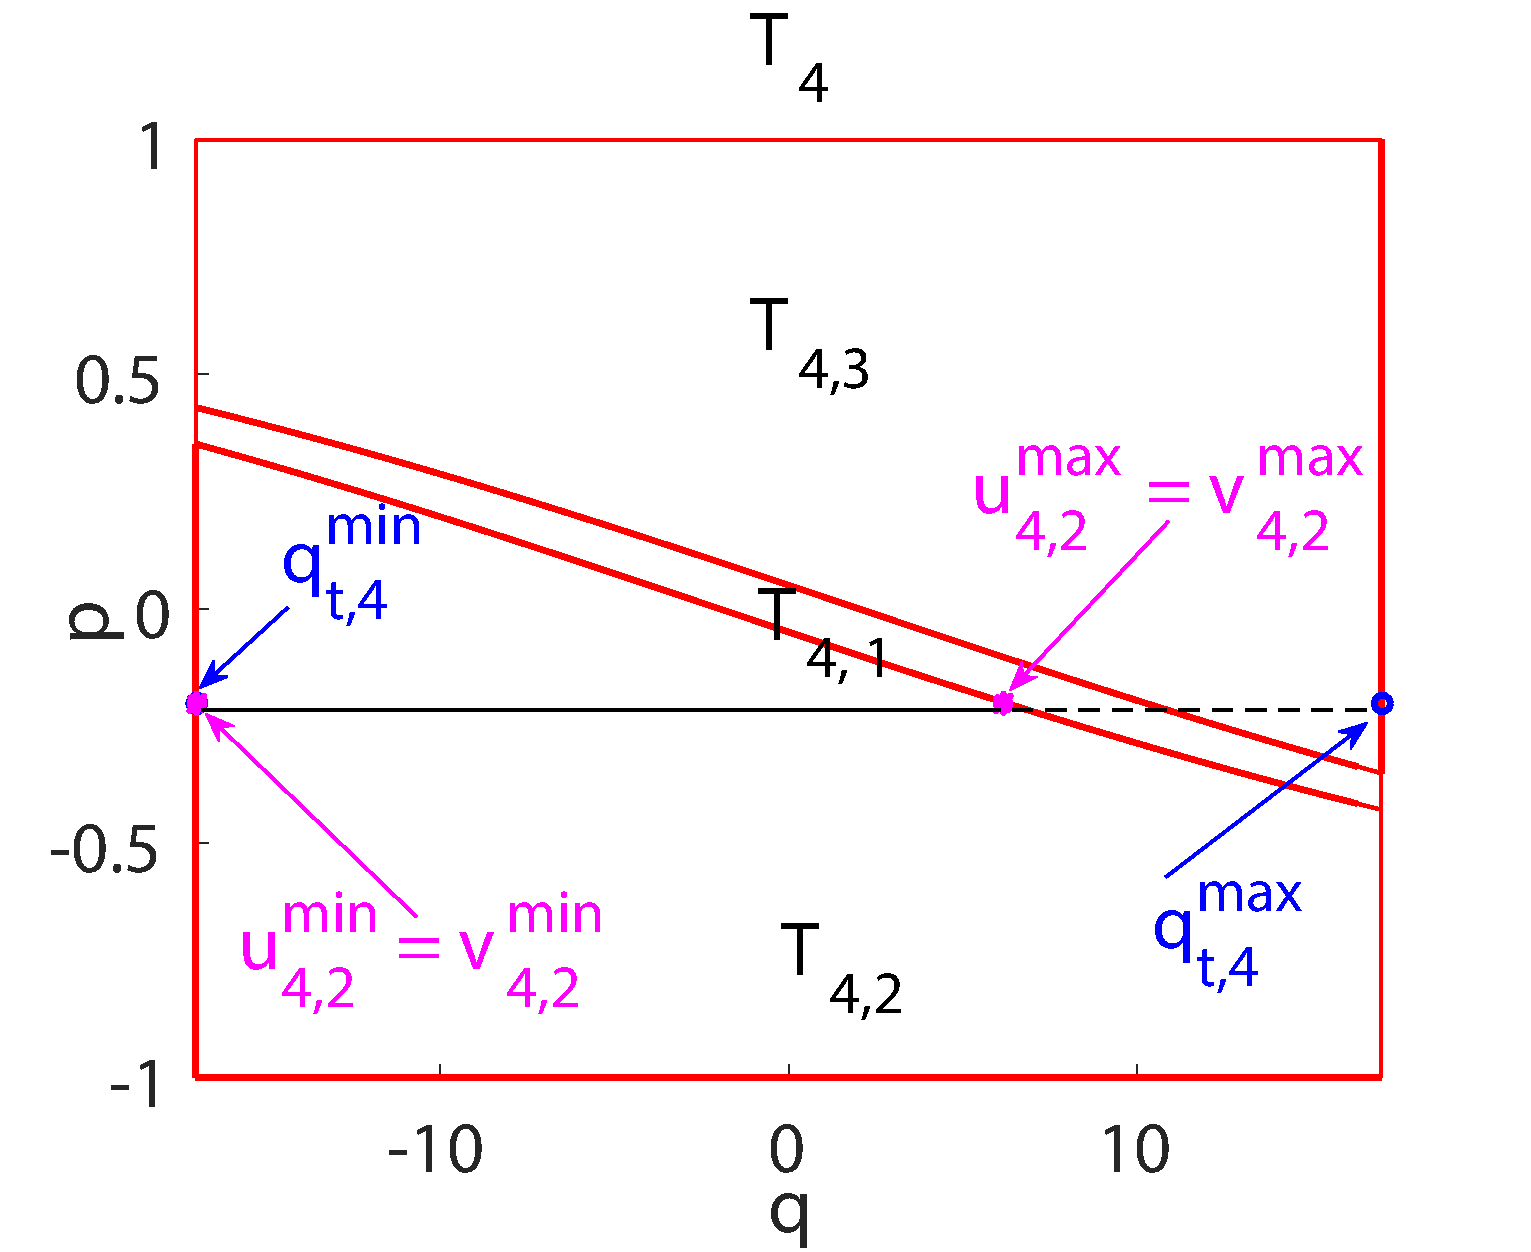
\includegraphics[width=\textwidth]{T4_2}
   \caption{\footnotesize{Target phase space of line $4$.
  The intersection points between the line $\variabile{p} = -0.2$ and $\partial$\set{T}{$4$,}{$2$} are $(\variabile{u}_{4,2}^{\textrm{min}}, \variabile{p})$ and
  $(\variabile{u}_{4,2}^{\textrm{max}}, \variabile{p})$. $\variabile{v}_{4,2}^{\textrm{min}}= \max \{\pos{t,}{$4$}^{\textrm{min}}, \variabile{u}_{4,2}^{\textrm{min}}\}$ and
  $\variabile{v}_{4,2}^{\textrm{max}}= \min \{\pos{t,}{$4$}^{\textrm{max}}, \variabile{u}_{4,2}^{\textrm{max}}\}$.\\}}
   \label{fig:T42}
 \end{minipage}
 \begin{minipage}[]{.48\textwidth}
   \centering
   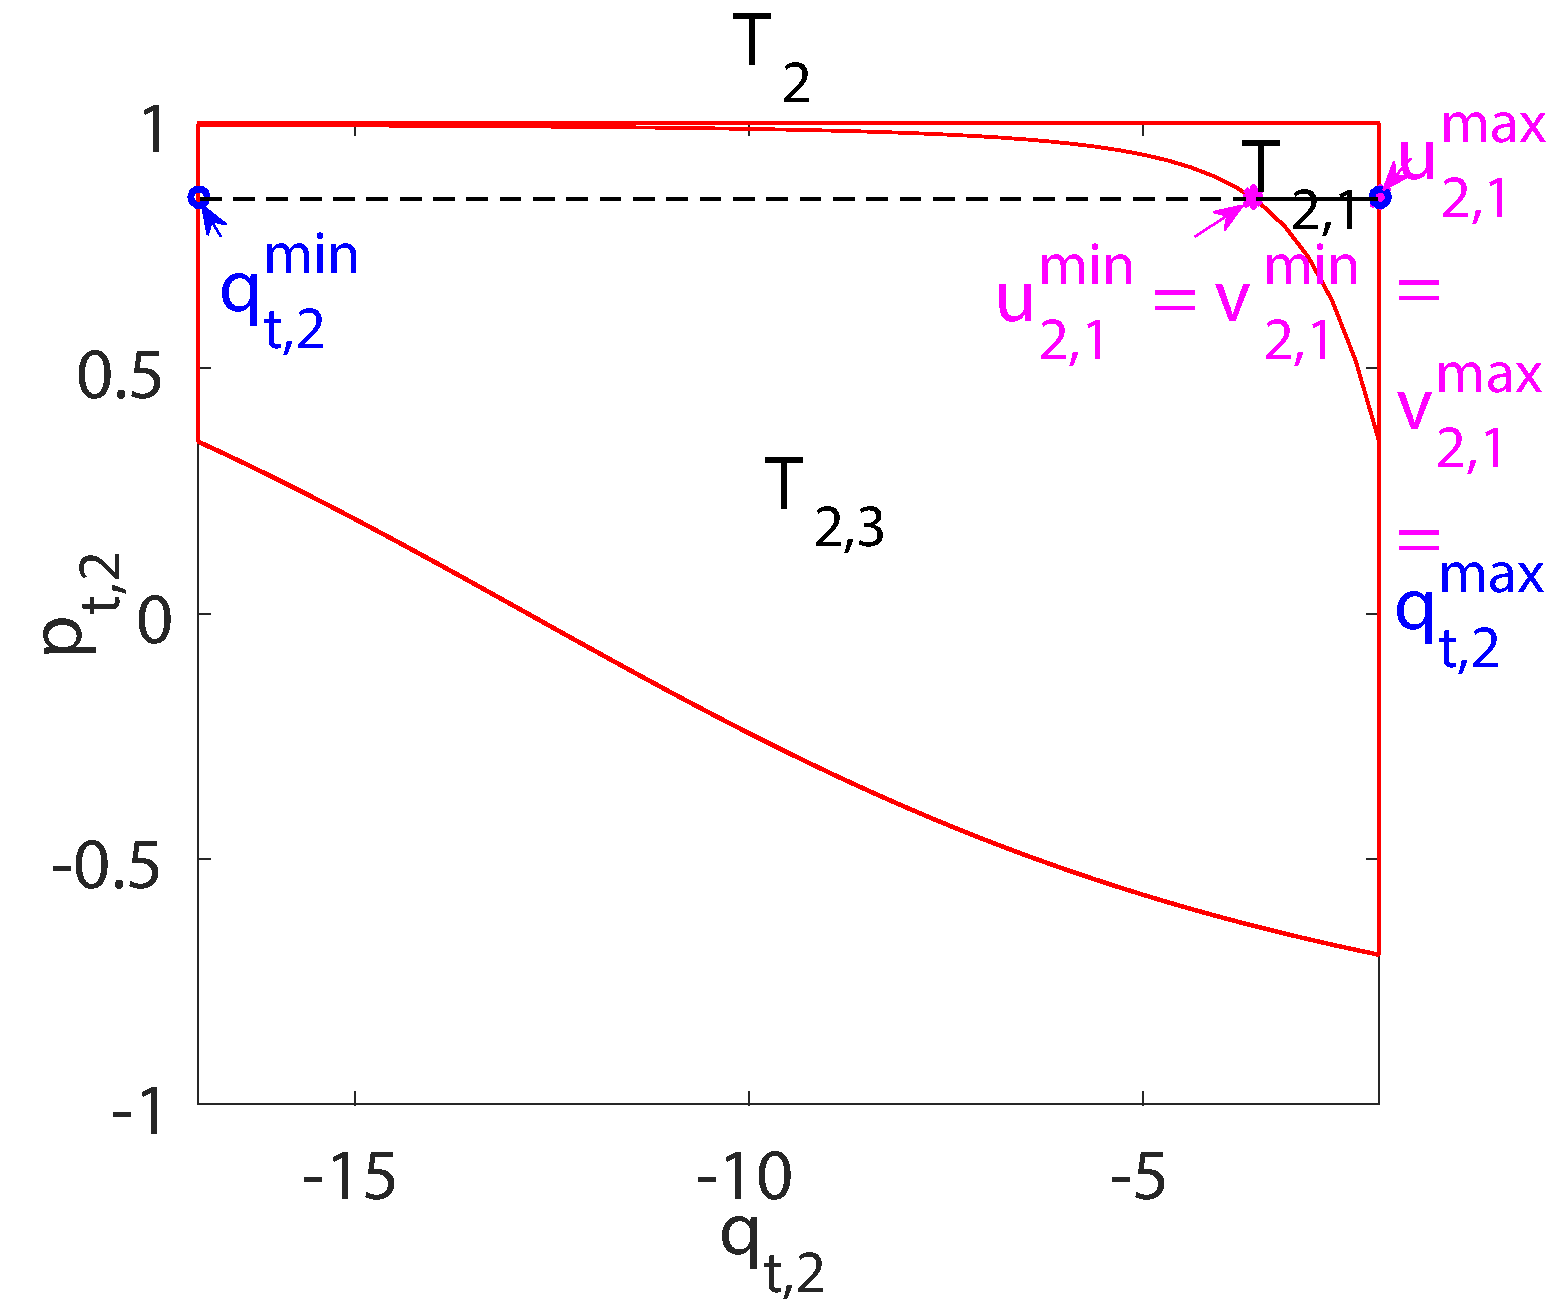
\includegraphics[width=\textwidth]{T2_1}
   \caption{\footnotesize{Target phase space of line $2$. The coordinates of the intersection points between line $\dir{t,}{$2$} = 0.82$ and $\partial$\set{T}{$2$,}{$1$} are
  $(\variabile{u}_{2,1}^{\textrm{min}}, \dir{t,}{$2$})$ and $(\variabile{u}_{2,1}^{\textrm{max}}, \dir{t,}{$2$})$.
  $\variabile{v}_{2,1}^{\textrm{min}}= \max \{\pos{t,}{$2$}^{\textrm{min}}, \variabile{u}_{2,1}^{\textrm{min}}\}$ and
  $\variabile{v}_{2,1}^{\textrm{max}}= \min \{\pos{t,}{$2$}^{\textrm{max}}, \variabile{u}_{2,1}^{\textrm{max}}\}$.}}
    \label{fig:T21}
 \end{minipage}
 \begin{minipage}[]{.48\textwidth}
  \centering
   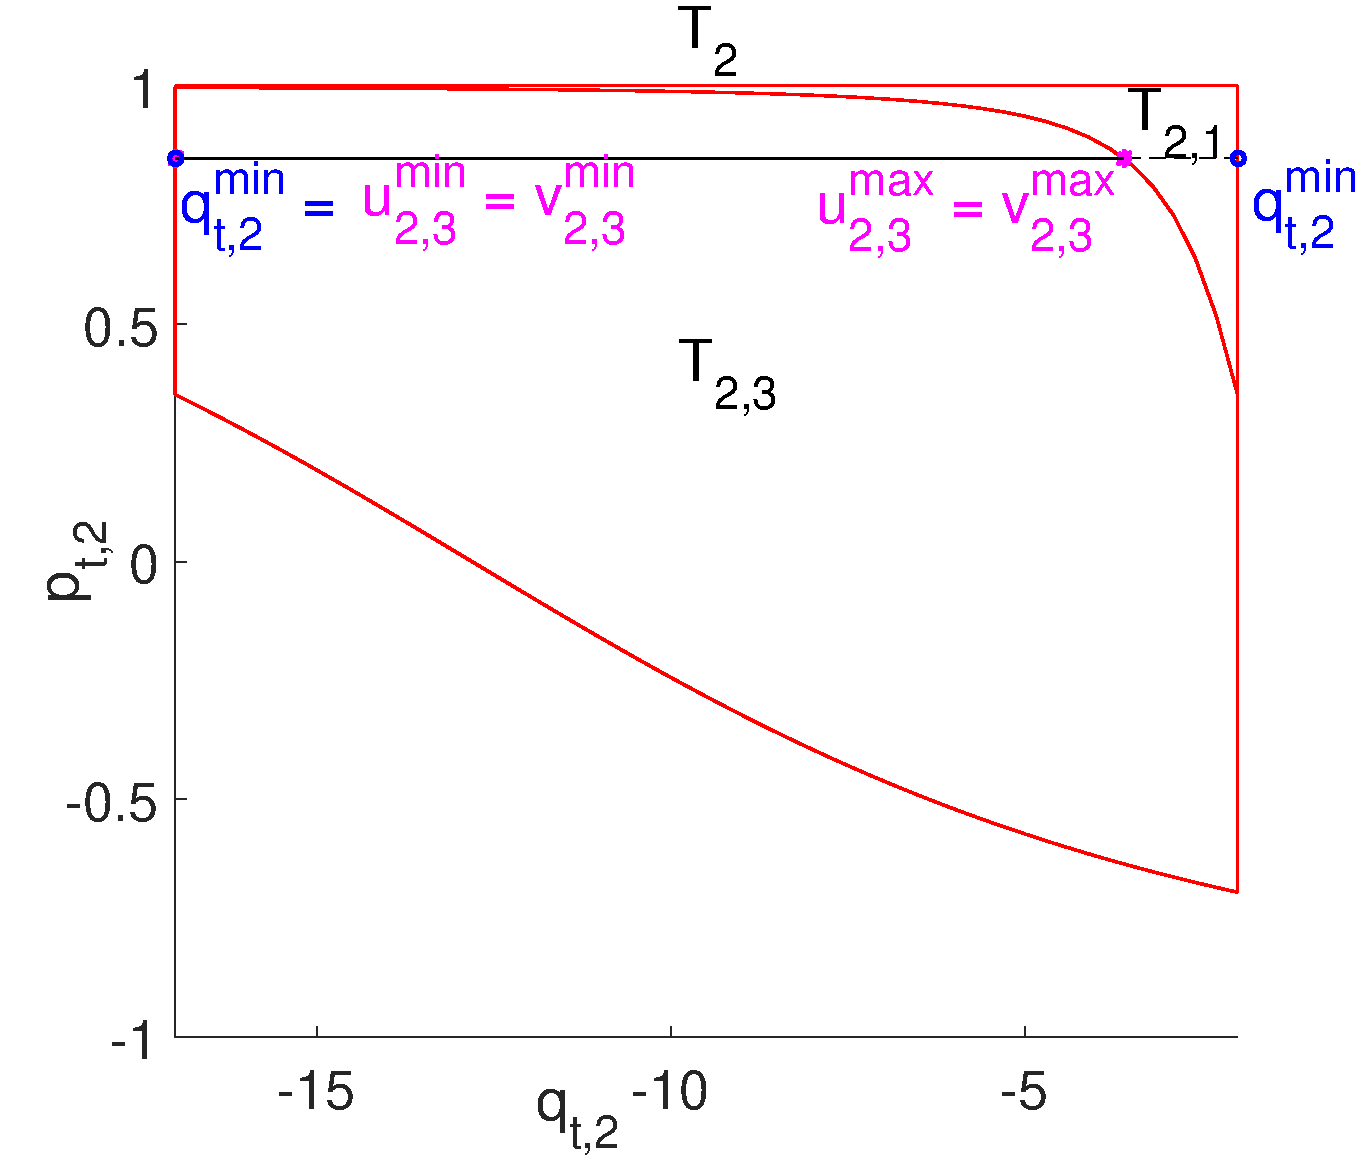
\includegraphics[width=\textwidth]{T2_2}
\caption{\footnotesize{Target phase space of line $2$.
  The coordinates of the intersection points between line $\dir{t,}{$2$}=0.82$ and $\partial$\set{T}{$2$,}{$3$} are
  $(\variabile{u}_{2,3}^{\textrm{min}}, 0.82)$ and $(\variabile{u}_{2,3}^{\textrm{max}}, 0.82)$.
  $\variabile{v}_{2,3 }^{\textrm{min}} = \max\{\variabile{u}_{2,3}^{\textrm{min}}, \pos{t,}{$2$}^{\textrm{min}}\}$ and
   $\variabile{v}_{2,3 }^{\textrm{max}} = \min\{\variabile{u}_{2,3}^{\textrm{max}}, \pos{t,}{$3$}^{\textrm{max}}\}$.}}
 \label{fig:T22}
 \end{minipage}
\hspace{3cm}
 \end{figure}
 \begin{figure}
\begin{minipage}[]{.48\textwidth}
   \centering
   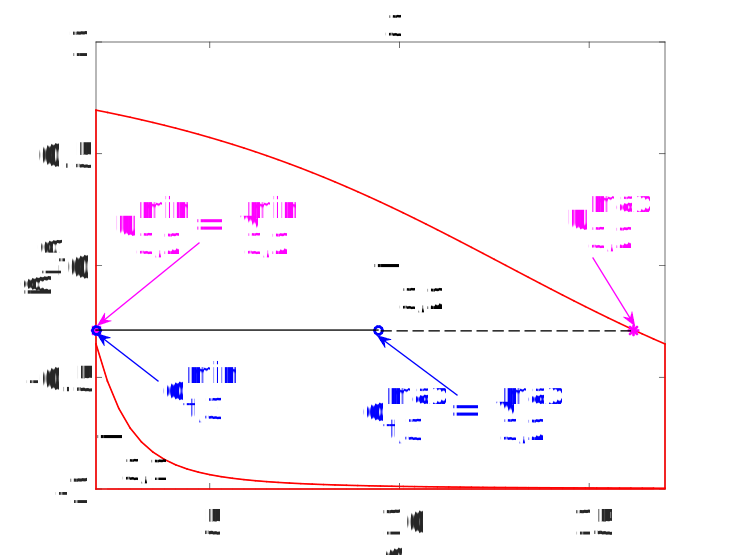
\includegraphics[width=\textwidth]{T3_1}
   \caption{\footnotesize{Target phase space of line $3$.
  The position coordinates of the intersection points between line line $ \dir{t,}{$3$} = -0.29$ and
  $\partial$\set{T}{$3$,}{$2$} are $\variabile{u}_{3,2}^{\textrm{min}}$ and $\variabile{u}_{3,2}^{\textrm{max}}$.
   $\variabile{v}_{3,2 }^{\textrm{min}} = \max\{\variabile{u}_{3,2}^{\textrm{min}}, \pos{t,}{$3$}^{\textrm{min}}\}$ and
   $\variabile{v}_{3,2 }^{\textrm{max}} = \min\{\variabile{u}_{3,2}^{\textrm{max}}, \pos{t,}{$3$}^{\textrm{max}}\}$.\\}}
   \label{fig:T31}
 \end{minipage}
 \begin{minipage}[]{.48\textwidth}
  \centering
   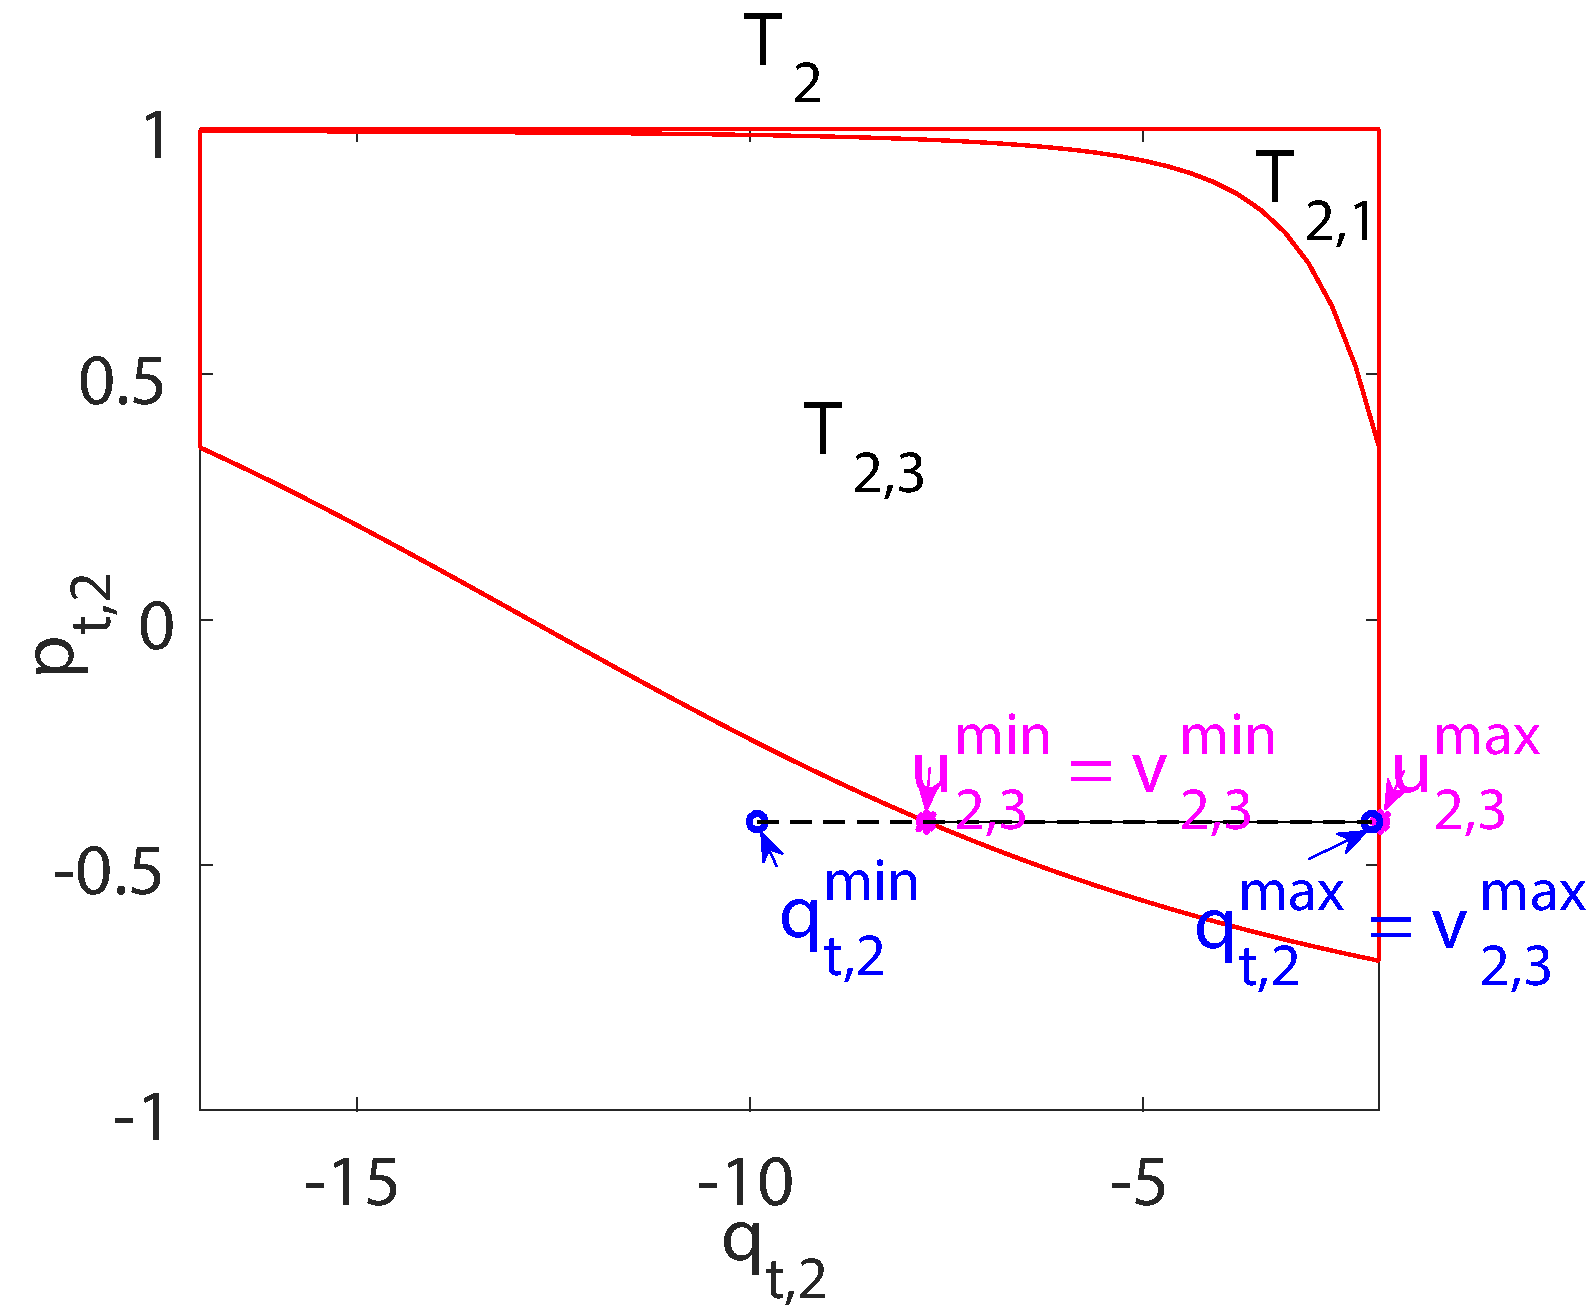
\includegraphics[width=\textwidth]{T2_3}
\caption{\footnotesize{Target phase phase of line $2$.
 The intersection points between line $\dir{t}{} = \dir{t,}{$2$}$ and $\partial$\set{T}{$2$,}{$3$} are
 $(\variabile{u}_{2,3}^{\textrm{min}}, \dir{t,}{$2$})$ and $(\variabile{u}_{2,3}^{\textrm{max}}, \dir{t,}{$2$})$.
 $\variabile{v}_{2,3 }^{\textrm{min}} = \max\{\variabile{u}_{2,3}^{\textrm{min}}, \pos{t,}{$2$}^{\textrm{min}}\}$ and
 $\variabile{v}_{2,3 }^{\textrm{max}} = \min\{\variabile{u}_{2,3}^{\textrm{max}}, \pos{t,}{$2$}^{\textrm{max}}\}$.\\}}
    \label{fig:T23}
 \end{minipage}
  \begin{minipage}[]{.48\textwidth}
   \centering
   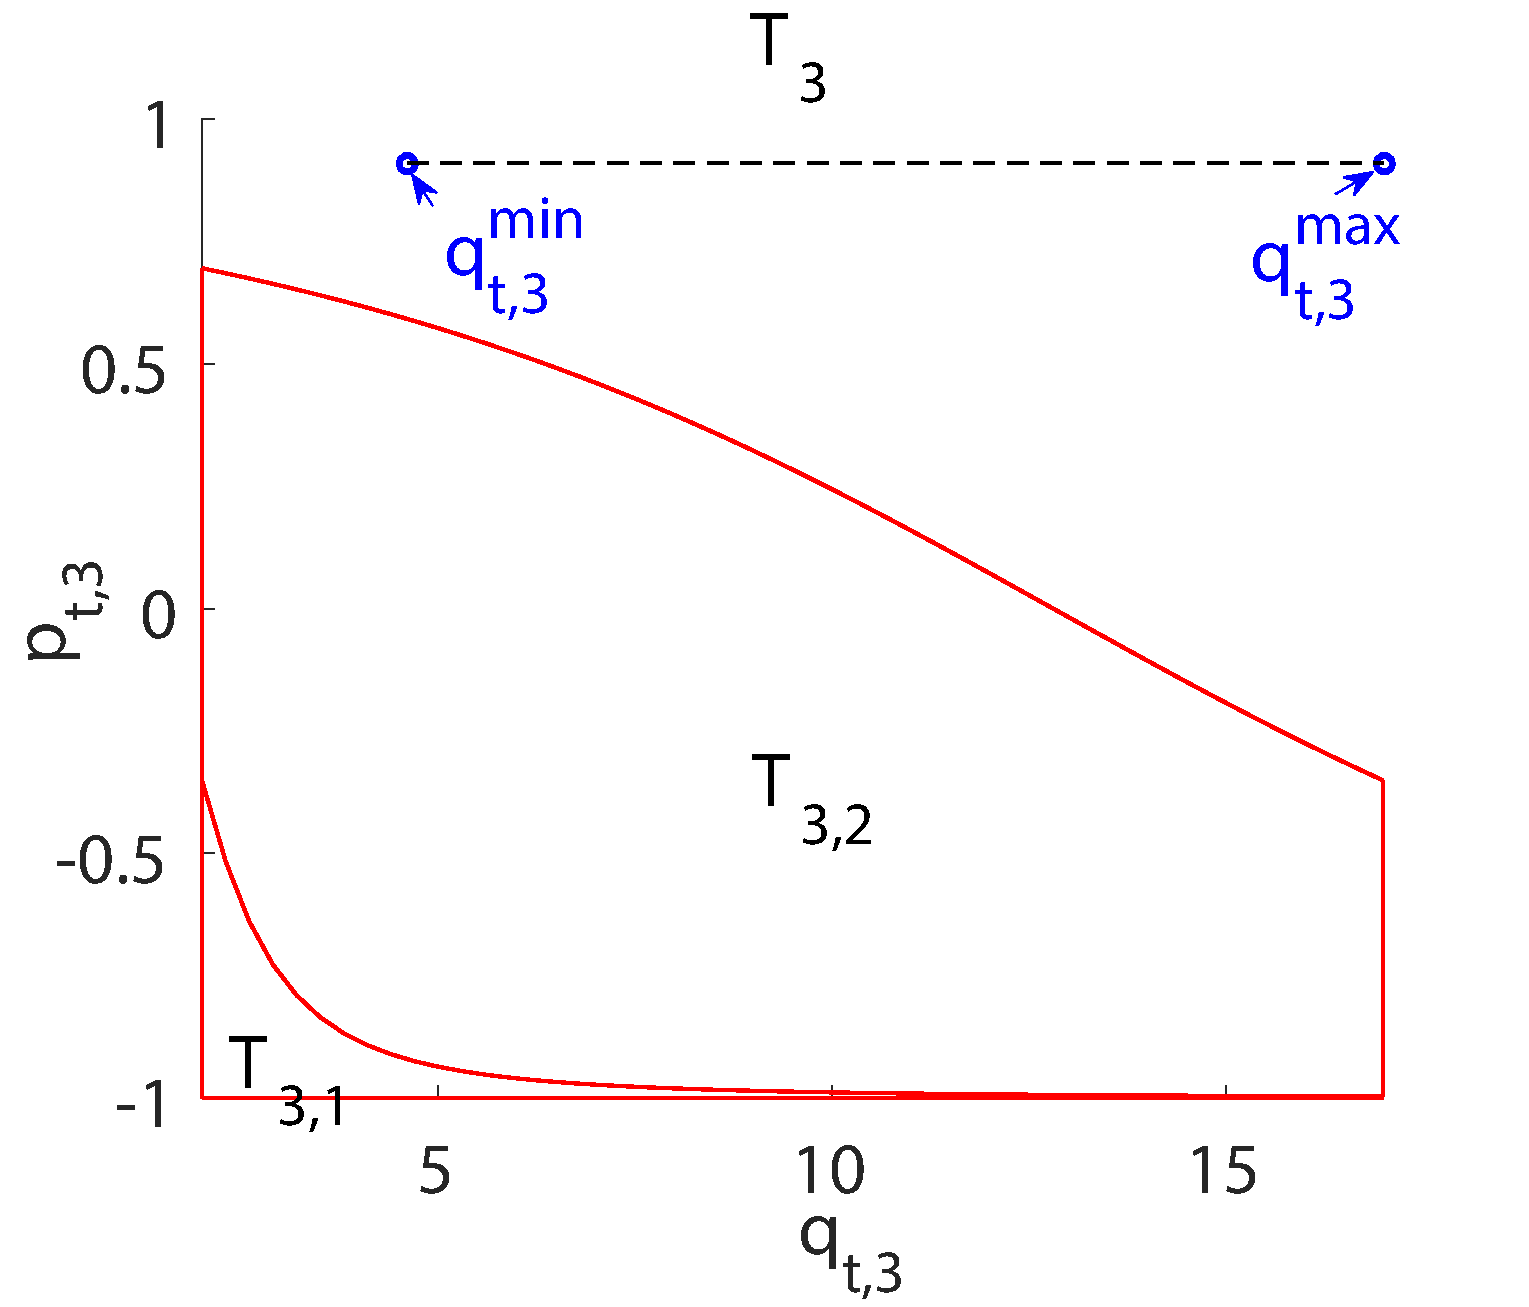
\includegraphics[width=\textwidth]{T3_2}
   \caption{\footnotesize{Target phase space of line $3$. 
  There are no intersection points of line $\dir{$3$,}{$2$}=0.91$
 with the boundaries $\partial$\set{T}{$3$,}{$2$} and $\partial$\set{T}{$3$,}{$1$}.
  The rays with coordinates inside the dotted segment hit again line $4$ after some reflections and, therefore, are not emitted by the source.}}
    \label{fig:T32}
 \end{minipage}
 \begin{minipage}[]{.48\textwidth}
   \centering
   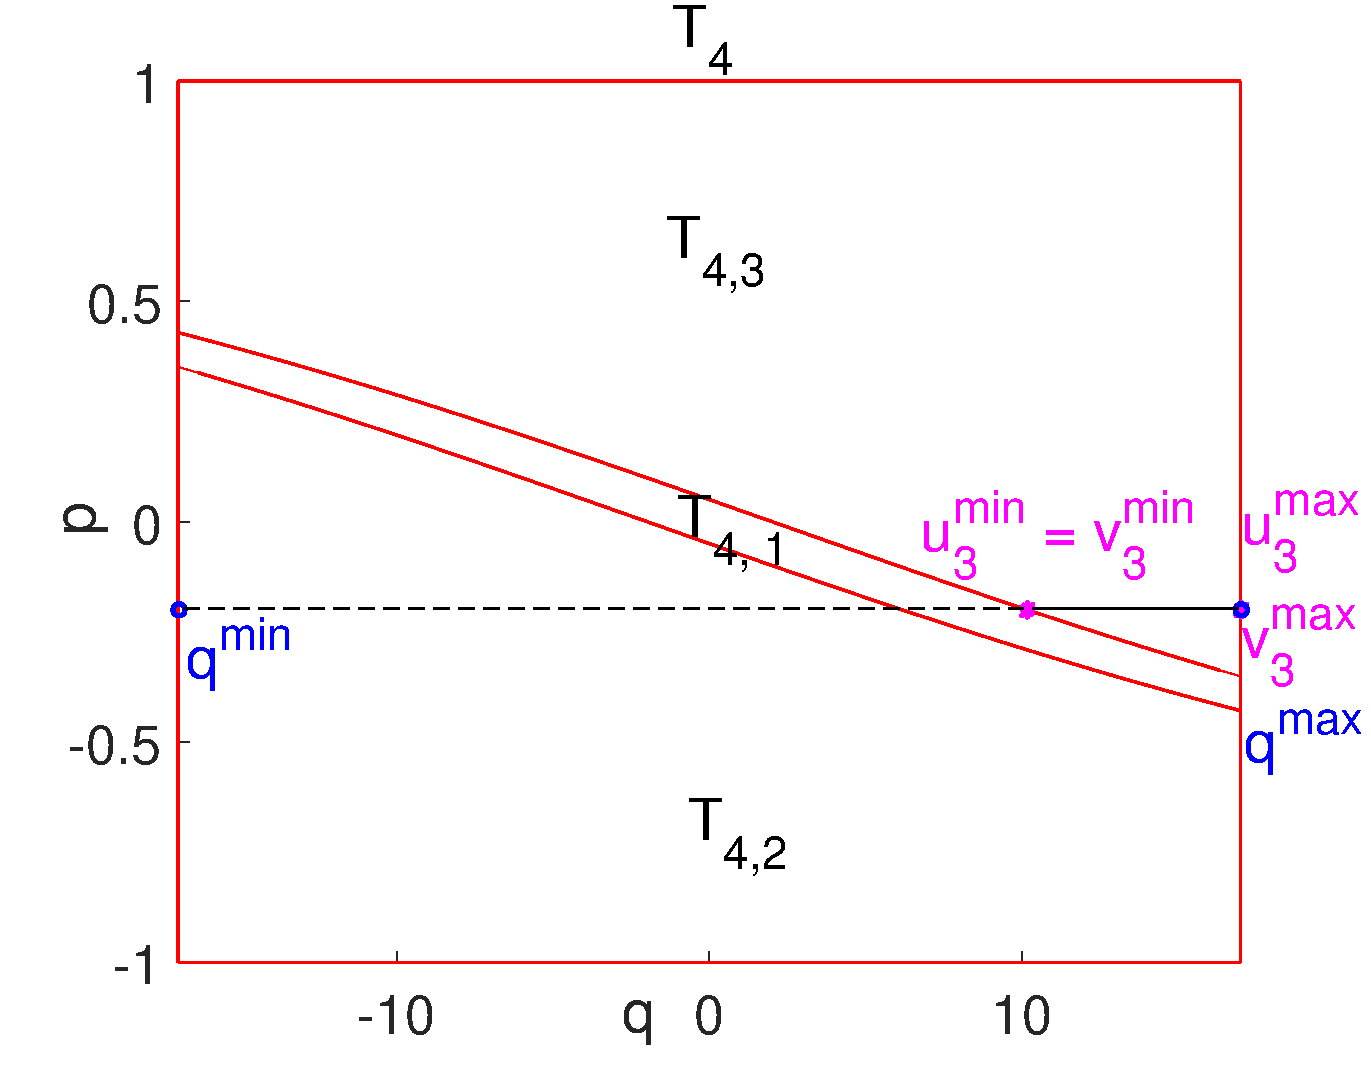
\includegraphics[width=\textwidth]{T4_3}
   \caption{\footnotesize{Target phase space of line $4$. $\pos{t,}{$4$}^{\textrm{min}} = -\variabile{b}$ and $\pos{t,}{$4$}^{\textrm{max}}= \variabile{b}$.
  The intersection points between line $\variabile{p} = -0.2$ and $\partial$\set{T}{$4$,}{$3$} are $(\variabile{u}_{4,3}^{\textrm{min}}, \variabile{p})$ and $(\variabile{u}_{4,3}^{\textrm{max}}, \variabile{p}).$ $\variabile{v}_{4,3}^{\textrm{min}} = \max\{\variabile{u}_{4,3}^{\textrm{min}}, \pos{t,}{$4$}^{\textrm{min}}\}$
  and $\variabile{v}_{4,3}^{\textrm{max}} = \min\{\variabile{u}_{4,3}^{\textrm{max}}, \pos{t,}{$4$}^{\textrm{max}}\}$.}}
   \label{fig:T43}
\end{minipage}
\hspace{3cm}
\end{figure}
\begin{algorithm}
\caption{Recursive procedure for the intensity calculation}\label{alg}
Initialize { $\lineaj=4,$  $\pos{t,}{$4$}^\textrm{\,min} = \variabile{q}^{\textrm{min}} =  -\variabile{b},$ 
 $\pos{t,}{$4$}^ \textrm{\,max}= \variabile{q}^{\textrm{max}}\variabile{b},$ $\dir{t, }{$4$} = \dir{}{} =  \const{constant},$  $\Pi = (4)$. }
\begin{algorithmic}[1]
\Procedure {Intensity computation}{ $\lineaj$, $\pos{t,}{\lineaj}^\textrm{\,min},$  $\pos{t,}{\lineaj}^ \textrm{\,max},$ $\dir{t, }{\lineaj},$  $\Pi$}
\For{$ \lineai =  1, 2, 3 $}
   \If{$\lineai\neq\lineaj$}
   \State Compute the intersection points 
    $(\variabile{u}_{j, i}^\textrm{\,min}, \dir{t,}{\lineaj})$ and $(\variabile{u}_{j, i}^\textrm{\,max}, \dir{t,}{\lineaj})$
   %between $\dir{t,}{\lineaj}$ and $\partial$\set{T}{\lineaj,}{\lineai}
 \State $\Pi\gets(\lineai, \Pi)$
           \State Compute 
%          \begin{equation*}
     $      [\variabile{v}_{\lineaj, \lineai}^\textrm{\,min}, \variabile{v}_{\lineaj, \lineai}^\textrm{\,max}] = [\variabile{u}_{\lineaj, \lineai}^\textrm{\,min}, \variabile{u}_{\lineaj, \lineai}^\textrm{\,max}]\cap
           [\pos{t,}{\lineaj}^\textrm{\,min}, \pos{t,}{\lineaj}^\textrm{\,min}] $
  %        \end{equation*}
       \If{($\lineai\neq 1)$  \& $ (\lineai\neq 4)$}
           \State Apply 
           \begin{equation*}
           \begin{aligned}
           (\pos{t,}{\lineai}^{\,1}, \dir{t,}{\lineai})& =\inversemap{R}{\lineai}{}\circ \inversemap{P}{\lineai,}{\lineaj}(\variabile{v}_{j,i}^\textrm{\,min}, \dir{t,}{\lineaj})  \\
           (\pos{t,}{\lineai}^{\,2}, \dir{t,}{\lineai}) & =\inversemap{R}{\lineai}{}\circ \inversemap{P}{\lineai,}{\lineaj}(\variabile{v}_{j,i}^\textrm{\,max}, \dir{t,}{\lineaj})
           \end{aligned}
           \end{equation*}
           \State Determine \begin{equation*}
\pos{t,}{\lineai}^\textrm{\,min}= \min\{\pos{t,}{\lineai}^{\,1}, \pos{t,}{\lineai}^{\,2}\} \mbox{ and }
\pos{t,}{\lineai}^\textrm{\,max}= \max\{\pos{t,}{\lineai}^{\,1}, \pos{t,}{\lineai}^{\,2}\}
\end{equation*}
          \State\Return{\Call{Intensity computation}{ $\lineai$, $\pos{t,}{\lineai}^\textrm{\,min},$  $\pos{t,}{\lineai}^ \textrm{\,max},$ $\dir{t, }{\lineai},$  $\Pi$}}
       \Else 
\If{\lineai=1}
              \If{$\lineaj\neq4$}
                 \State Apply 
\begin{equation*}
\begin{aligned}
(\pos{s,}{1}^{\,1}, \dir{s,}{1})& = \inversemap{P}{1,}{\lineaj}(\variabile{v}_{\lineaj,1 }^\textrm{\,min}, \dir{t,}{\lineaj})  \\
(\pos{s,}{1}^{\,2}, \dir{s,}{1}) & =\inversemap{P}{1,}{\lineaj}(\variabile{v}_{\lineaj, 1}^\textrm{\,max}, \dir{t,}{\lineaj})\\
(\pos{}{}^{1}(\Pi, \dir{}{}), \dir{}{})&= \mapnumb{M}_{1,4}(\Pi)(\pos{s,}{1}^{\,1}, \dir{s,}{1})\\
(\pos{}{}^{2}(\Pi, \dir{}{}), \dir{}{})&= \mapnumb{M}_{1,4}(\Pi)(\pos{s,}{1}^{\,2}, \dir{s,}{1})
\end{aligned}
\end{equation*}
%\State Apply 
%\begin{equation*}
%\begin{aligned}
% (\pos{}{}^{1}(\Pi, \dir{}{}), \dir{}{})&= \mapnumb{M}_{1,4}(\Pi)(\pos{s,}{1}^{\,1}, \dir{s,}{1})\\
% (\pos{}{}^{2}(\Pi, \dir{}{}), \dir{}{})&= \mapnumb{M}_{1,4}(\Pi)(\pos{s,}{1}^{\,2}, \dir{s,}{1})
%\end{aligned}
%\end{equation*}
\State Calculate
\begin{equation*}
\begin{aligned}
\pos{}{}^\textrm{\,min}(\Pi,\dir{}{})&= \min\{\pos{}{}^{\,1}, \pos{}{}^{\,2}\}, \\ 
\pos{}{}^\textrm{\,max}(\Pi,\dir{}{})&= \max\{\pos{}{}^{\,1}, \pos{}{}^{\,2}\},
\end{aligned}
\end{equation*}
\State where $\pos{}{}^{\,1} := \pos{}{}^{\,1}(\Pi, \dir{}{})$ and $\pos{}{}^{\,2} := \pos{}{}^{\,2}(\Pi, \dir{}{})$.
                 \State\Return{$I(\variabile{p})= I(\variabile{p})+\variabile{q}^\textrm{\,min}(\Pi, \dir{}{})-\variabile{q}^\textrm{\,max}(\Pi, \dir{}{}).$}
                 \Else
                 \begin{equation*}
                    %   \begin{aligned}
                       \variabile{q}^\textrm{\,min}(\Pi, \dir{}{}) = \variabile{v}_{4, \lineaj}^\textrm{\,min}\mbox{ and }
                       \variabile{q}^\textrm{\,max}(\Pi, \dir{}{}) = \variabile{v}_{4, \lineaj}^\textrm{\,max}
                    %   \end{aligned}
                       \end{equation*}
                  \State\Return{$I(\variabile{p})= I(\variabile{p})+\variabile{q}^\textrm{\,min}(\Pi, \dir{}{})-\variabile{q}^\textrm{\,max}(\Pi, \dir{}{}).$}
              \EndIf    
\Else \pagebreak
\State \Return $I(\variabile{p})$
\EndIf
        \EndIf
     \EndIf
\EndFor
\EndProcedure
\end{algorithmic}
\end{algorithm}
 \indent In the next section we provide the numerical results for the two-faceted cup. 

\section{Results for the two-faceted cup}
To demonstrate the accuracy of the method, a comparison with the ray tracing approach is provided.
In particular, we compare our method with MC ray tracing.
The MC intensity is computed tracing randomly a large number of rays from the source to the target of the system.
Then, a partitioning $P:-1 = \variabile{p}^0 < \cdots< \variabile{p}^\textrm{Nb} = 1$ of the interval $[-1,1]$ is considered, where $\textrm{Nb}$ indicates the number of bins in the partitioning.
The MC intensity along the direction $\variabile{p}\in[\variabile{p}^\variabile{h}, \variabile{p}^{\variabile{h}+1}]$ is given by the ratio of the number of rays $\textrm{Nr}[\variabile{p}^\variabile{h}, \variabile{p}^{\variabile{h}+1}]$ that arrive at the bin $[\variabile{p}^\variabile{h}, \variabile{p}^{\variabile{h}+1}]$ and the total number of rays $\textrm{Nr}[-1, 1]$ that arrive at the target for every $\variabile{p}\in[\variabile{p}^\variabile{h}, \variabile{p}^{\variabile{h}+1}]$ as defined in Equation (\ref{eq:normalized_MC_intensity}). Hence, the MC intensity is piecewise constant. Note that $\hat{I}_{\textrm{MC}}$ is normalized. In order to compute the intensity distribution for all the directions, the partitioning $P$ of the target is considered. Then, the procedure explained above is repeated for $\Big(\variabile{p}^{\variabile{h}+1/2} = \frac{1}{2}(\variabile{p}^{\variabile{h}+1}+\variabile{p}^\variabile{h})\Big)_{\variabile{h} = 0, \cdots, \textrm{Nb}-1}$ and the MC intensity is calculated over every bin. The profile of the MC intensity is depicted in Fig. \ref{fig:intensity_cup} with a blue line. There the intensity is calculated tracing $10^7$ rays and taking $\textrm{Nb} = 100$.\\
\indent Next, we compute the intensity at the target employing the PS ray mapping method. Using the procedure explained in Section \ref{sec:algorithm}, we are able to detect all the possible paths $\Pi$ that a ray can follow during the propagation through the system. 
For the two-faceted cup $5$ different paths are found. Given a path $\Pi$, the coordinates $(\variabile{q}^\textrm{min}(\Pi, \variabile{p}^ \variabile{h}), \variabile{p}^ \variabile{h})$ and $(\variabile{q}^\textrm{\,max}(\Pi, \variabile{p}^ \variabile{h}), \variabile{p}^\variabile{h})$ of the rays located on $\partial \mbox{\set{R}{}{}}(\Pi)$ are determined for every $\variabile{p} = (\variabile{p}^\variabile{h})_{\variabile{h}=0, \cdots, \textrm{Nb}}$ where the values $\variabile{p}^\variabile{h}$ are given from the partitioning $P$ used for MC ray tracing. These rays are depicted in Fig. \ref{fig:final_T}, where all the rays that follow the same path are shown with the same color. The PS intensity is obtained from Eq. (\ref{eta2}). Note from Fig. $\ref{fig:final_T}$ that only $2\textrm{Nb}$ rays need to be traced through the system for the intensity computation.
The averaged normalized PS intensity is given by Equation (\ref{eq:normalized_PS_intensity})
%\begin{equation}\label{eq:intensity}
% \hat{I}_{\textrm{PS}}(\variabile{p}^{\variabile{h}+1/2}) = \frac{\int_{\variabile{p}^\variabile{h}}^{\variabile{p}^{\variabile{h}+1}}{\lineai}_{PS}(\variabile{p})\textrm{d}\variabile{p}}{\int_{-1}^{1}{\lineai}_{PS}(\variabile{p})\textrm{d}\variabile{p}}\,,
% \end{equation}
%for $\variabile{h} = 0,1, \cdots, \textrm{Nb}-1,$
 where the integrals are calculated using the trapezoidal rule.
\begin{figure}[t]
  \begin{center}
  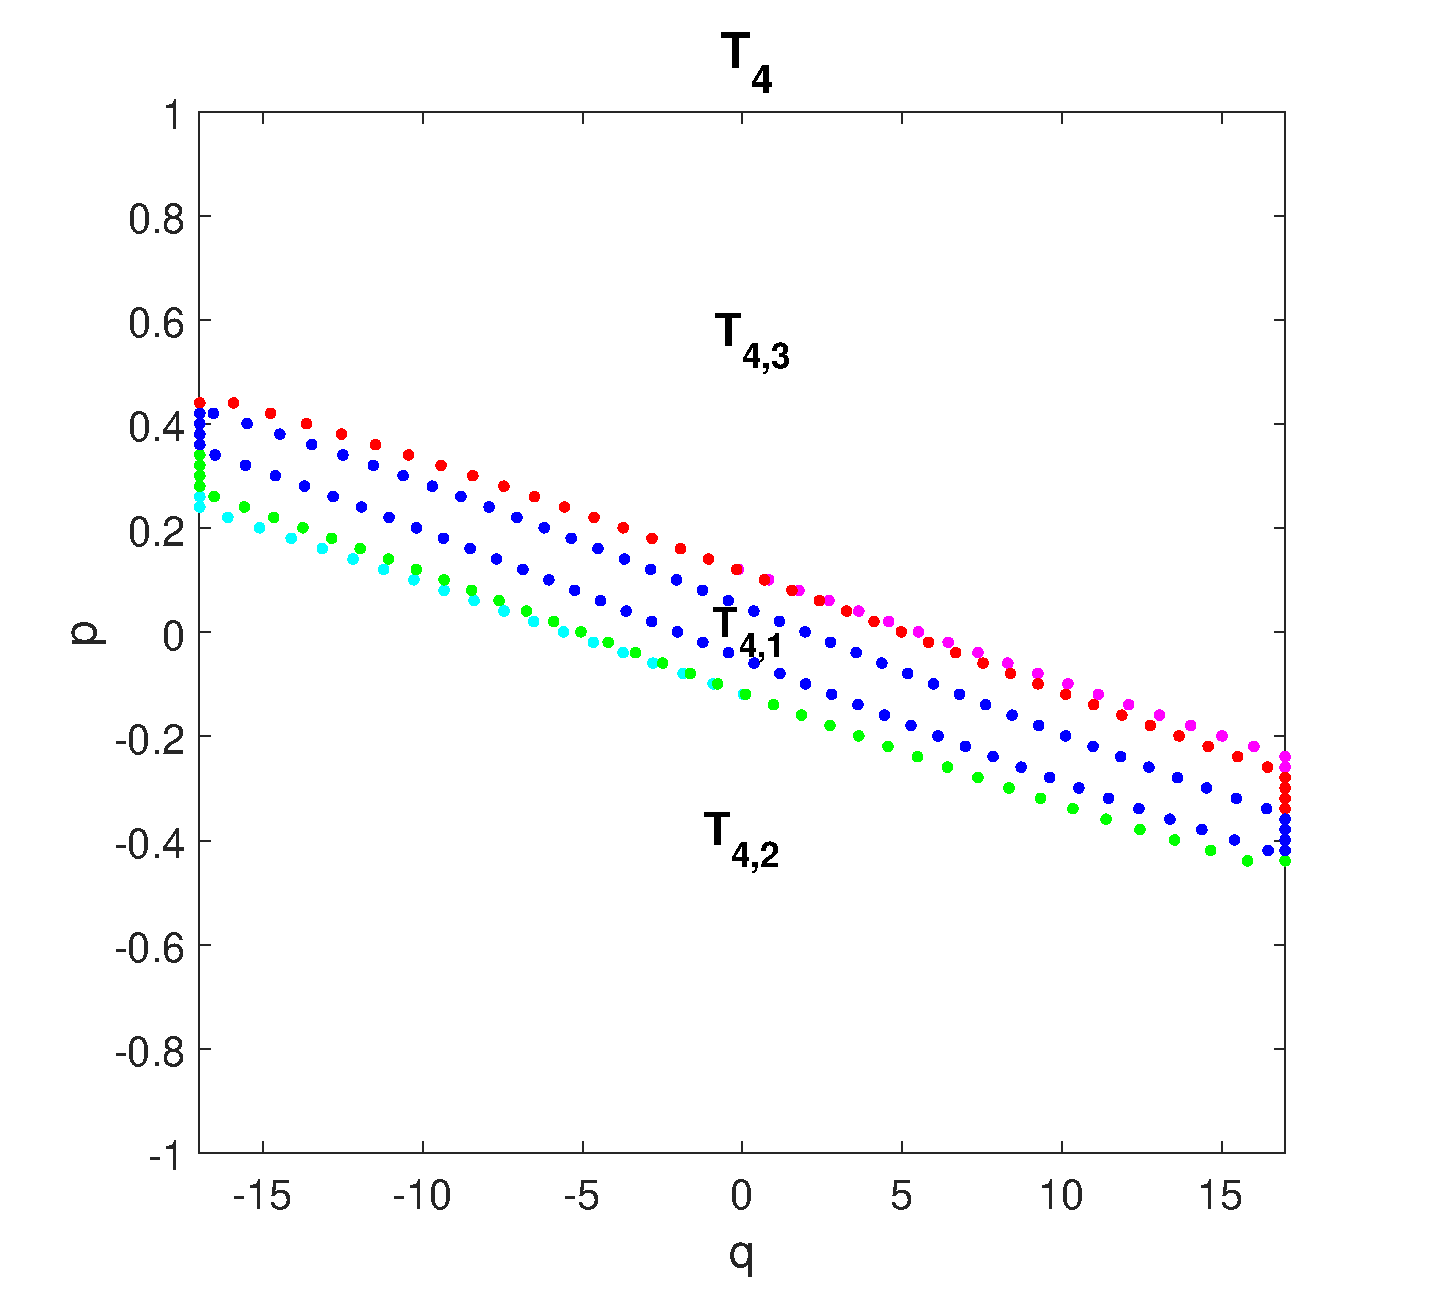
\includegraphics[scale=.4]{final_T}
  \end{center}
  \caption{\textbf{Target phase space of the two-faceted cup divided into $100$ bins.}
  Five different paths are found. The rays with coordinates $(\variabile{q}^\textrm{\,min}, \variabile{p})$ and $(\variabile{q}^\textrm{\,max}, \variabile{p})$ in \set{T}{$4$}{} that are located at the boundaries $\partial \mbox{\set{R}{}{}}(\Pi)$ are depicted with dots, the color of the dots depends on the path $\Pi$ followed by the rays.
  Using the ray mapping method, only these rays need to be traced from $\point{S}$ to $\point{T}$ for the intensity computation.}
  \label{fig:final_T}
\end{figure} 
The profile of the PS intensity is depicted in in Fig. \ref{fig:intensity_cup} with the dotted green line. 
\\ \indent For the two-faced cup, the intensity can be computed analytically.
This intensity is taken as the reference intensity  $\hat{I}_{\mbox{ref}}$ and, it is depicted in Fig. \ref{fig:intensity_cup} with a red line.
The results in Fig. \ref{fig:intensity_cup} show that all the intensity's profiles are all similar to each other. Therefore, we can claim that our method computes the intensity correctly. 
 \\ \indent
In order to compare the speed of convergence of the two methods, we consider the error between the approximate intensities $\hat{I}_{\textrm{A}}$ ($\textrm{A} = \textrm{MC}, \textrm{PS}$) and the exact intensity $\hat{I}_{\mbox{exact}} = \hat{I}_{\mbox{ref}}$ from Equation (\ref{eq:error})
%\begin{equation}\label{error}
%\mbox{error} = \frac{\sum_{\variabile{h} = 1}^{\textrm{Nb}}| \hat{I}_{\textrm{A}}(\variabile{p}^\variabile{h}) - \hat{I}_{\textrm{ref}}(\variabile{p}^\variabile{h})|}{\textrm{Nb}}\,.
%\end{equation}
As the accuracy of the ray tracing method depends on the number of rays traced, the MC intensity is calculated for increasing numbers of rays traced through the system and, the error between the approximate intensity and the reference intensity is computed using Equation (\ref{eq:error}). In Fig. $\ref{fig:error_cup}$ the behavior of the MC error as a function of the CPU-time is depicted with the blue line. Increasing the number of rays the MC error decreases proportionally to the inverse of the square root of the number of rays traced. Next, the PS error is computed using Equation (\ref{eq:error}). It is depicted in Fig. $\ref{fig:error_cup}$ with the green dot. From the numerical results shown in Fig. $\ref{fig:error_cup}$ we can conclude that the PS ray mapping method is able to compute the output intensity of the two-faceted cup exactly. Also, it is much faster than the classical ray tracing approach when an error smaller than $10^{-4}$ is required.
\begin{figure}[h]
  \begin{center}
  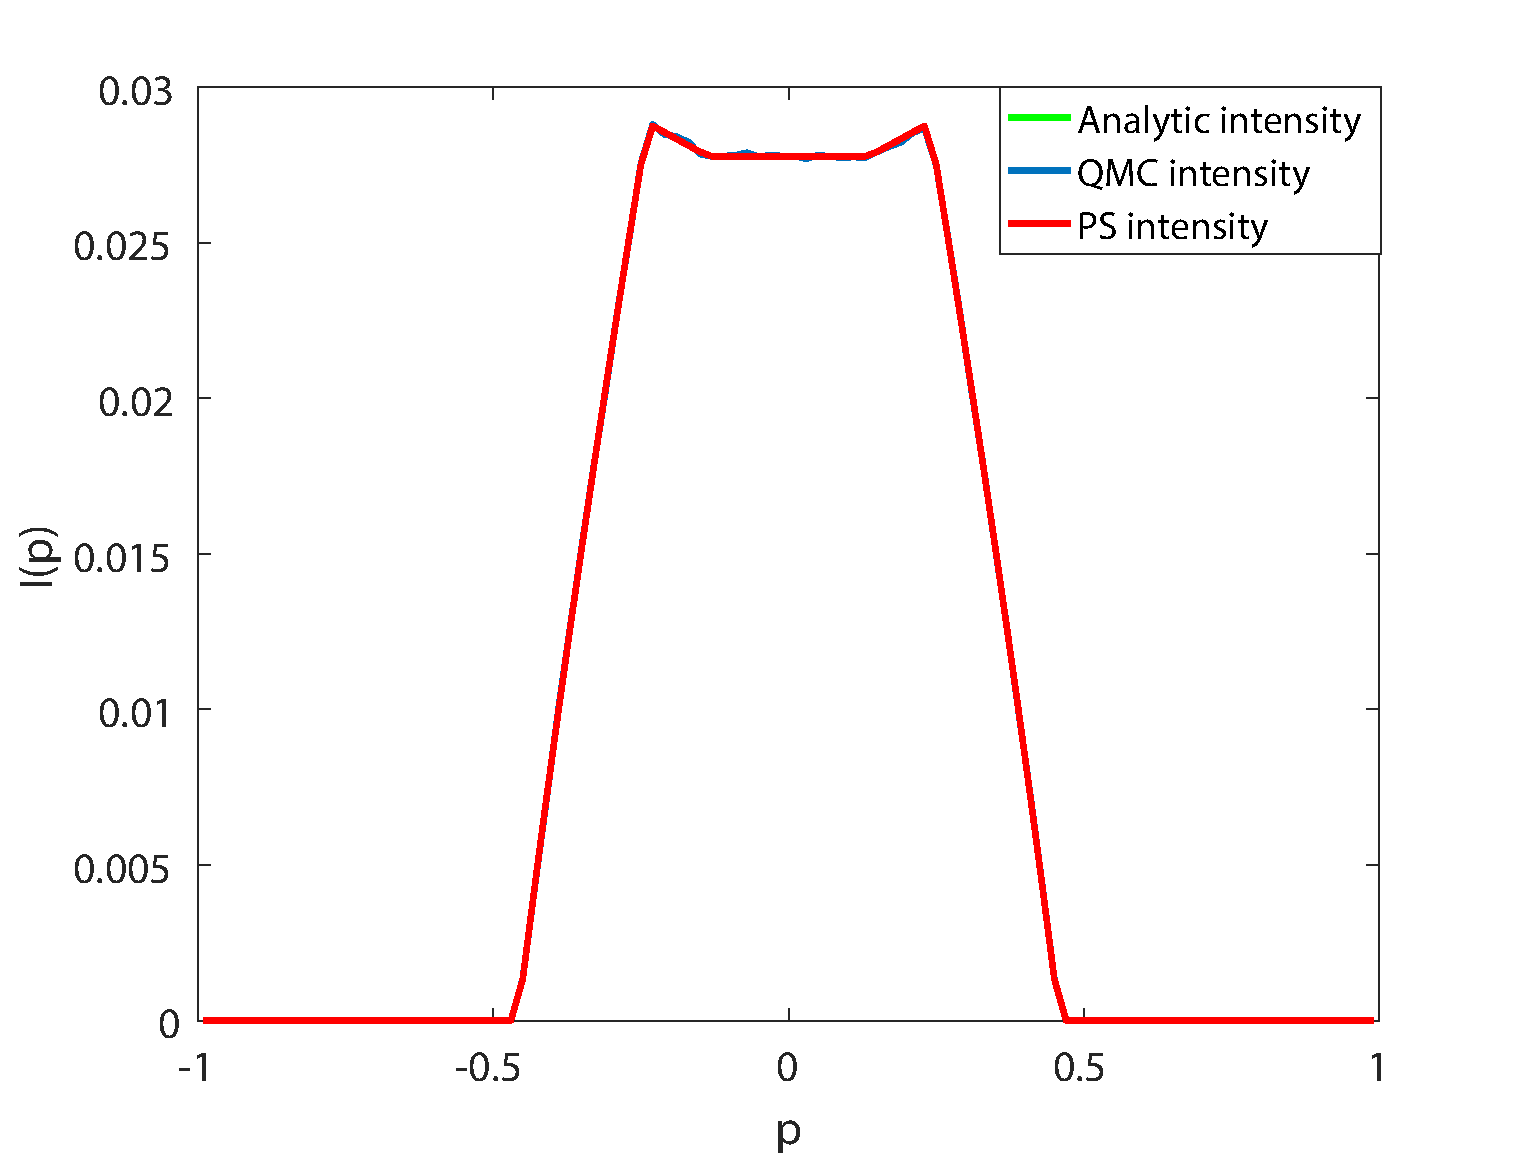
\includegraphics[scale=.4]{intensity_cup_raymapping}
  \end{center}
  \caption{\textbf{Intensities for the two-faceted cup.} The intensities found with three different approaches are shown.}
  \label{fig:intensity_cup}
\end{figure}
\begin{figure}[h]
  \begin{center}
  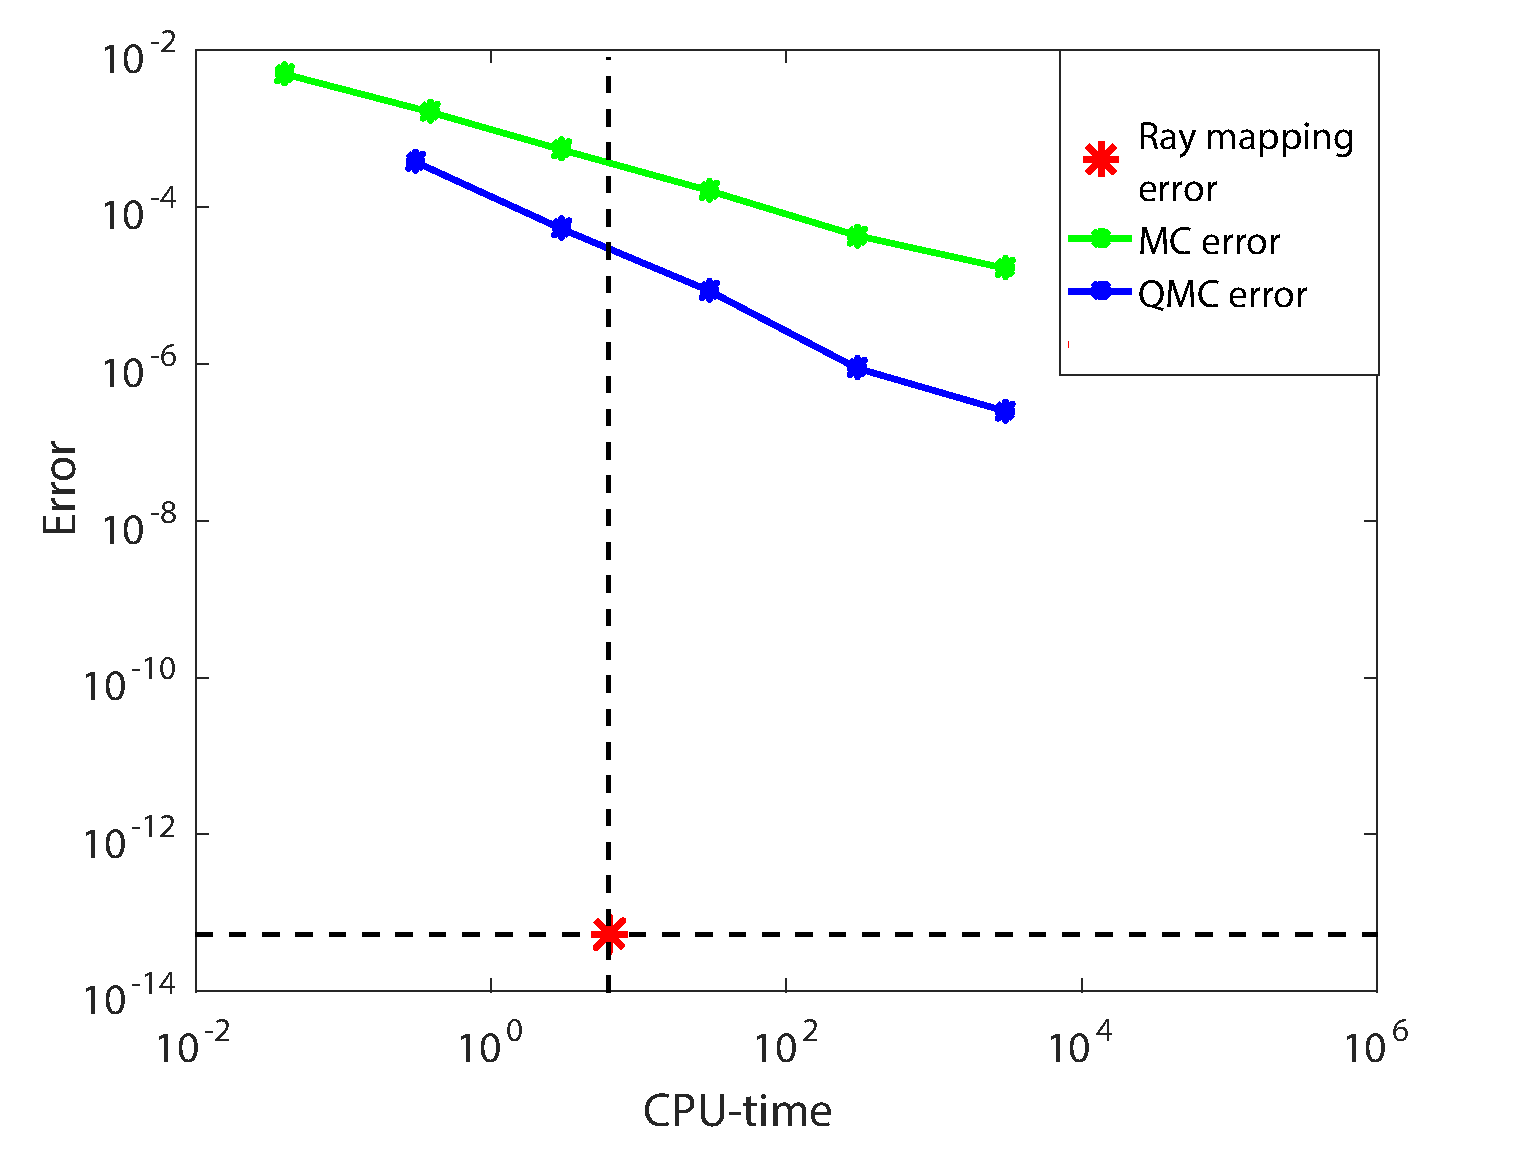
\includegraphics[scale=.4]{error_cup_raymapping}
  \end{center}
  \caption{\textbf{Errors for the two-faceted cup.} The errors is depicted as a function of the CPU time (in seconds) and it is shown in a logarithmic scale.}
  \label{fig:error_cup}
\end{figure}

\section{Results for the multi-faceted cup}


\label{sec:Generalization}
The method can be generalized to more complicated optical systems.
In particular, it can be used for all systems formed by straight line segments.
The goal of this section is to show the generalization of the method to the multi-faced cup which is a system with many left and right segments as reflectors.
The design of this system is explained below. \\ \indent
A multi-faceted cup is an optical system formed by a source, a target and $\textrm{Nl}-2$ reflectors, where \textrm{Nl} is the number of optical line segments that form the system.
Defining a Cartesian coordinate system $(\variabile{x}, \variabile{z})$, the multi-faceted cup is symmetric with respect to the optical axis (\variabile{z}-axis). An example of this system is depicted in Fig. \ref{fig:multifacetedcup} where all the lines are labeled with numbers.
The source $\point{S}= [-\variabile{a}, \variabile{a}]$ (line $1$) and the target $\point{T}= [-\variabile{b}, \variabile{b}]$ (line $22$) are two segments both perpendicular to the optical axis, with $\variabile{a}=2$ and $\variabile{b}=17$.
$\point{S}$ is located at the height $\variabile{z}=0$ while $\point{T}$ has a height $\variabile{z}=40$.
Both sides of the system are divided into $10$ segments which connect $\point{S}$ with $\point{T}$.
The $10$ adjacent segments at the left of the system (lines $2, \cdots, 11$) connect the left extreme of the source with the left extreme of the target.
Similarly, $10$ adjacent segments at the right of the system (lines $12, \cdots, 21$) connect the right extreme of the source with the right extreme of the target.
These segments are designed as follows. The intervals $[-\variabile{b}, -\variabile{a}]$ and $[\variabile{a}, \variabile{b}]$ are divided into $10$ subintervals of the same length $(\variabile{b}-\variabile{a})/10$.
The \variabile{x}-coordinates of the end points of the line segments $12, \cdots, 21$ are equal to the \variabile{x}-coordinates of the subintervals of $[\variabile{a},\variabile{b}]$, while the \variabile{x}-coordinates of the end points of the line segments $2, \cdots, 11$ are equal to the \variabile{x}-coordinates of the subintervals of $[-\variabile{a},-\variabile{b}]$.
The \variabile{z}-coordinates of every end point of the line segments $2, \cdots, 21$  are given substituting their $\variabile{x}$-coordinates into the equation of the parabola whose symmetric axis is equal to the \variabile{z}-axis and that passes through the
points $(-17,40)$ and $(17,40)$. The $20$-faceted cup is now well defined and can be seen as an approximation of a parabolic reflector.
All the optical lines \lineai with $\lineai \in \{1, \cdots, 22\}$ are located in air, therefore the refractive index $\variabile{n}_{\lineai}=1$ for every \lineai.
\begin{figure}[h]
\centering
\label{fig:multifacetedcup}
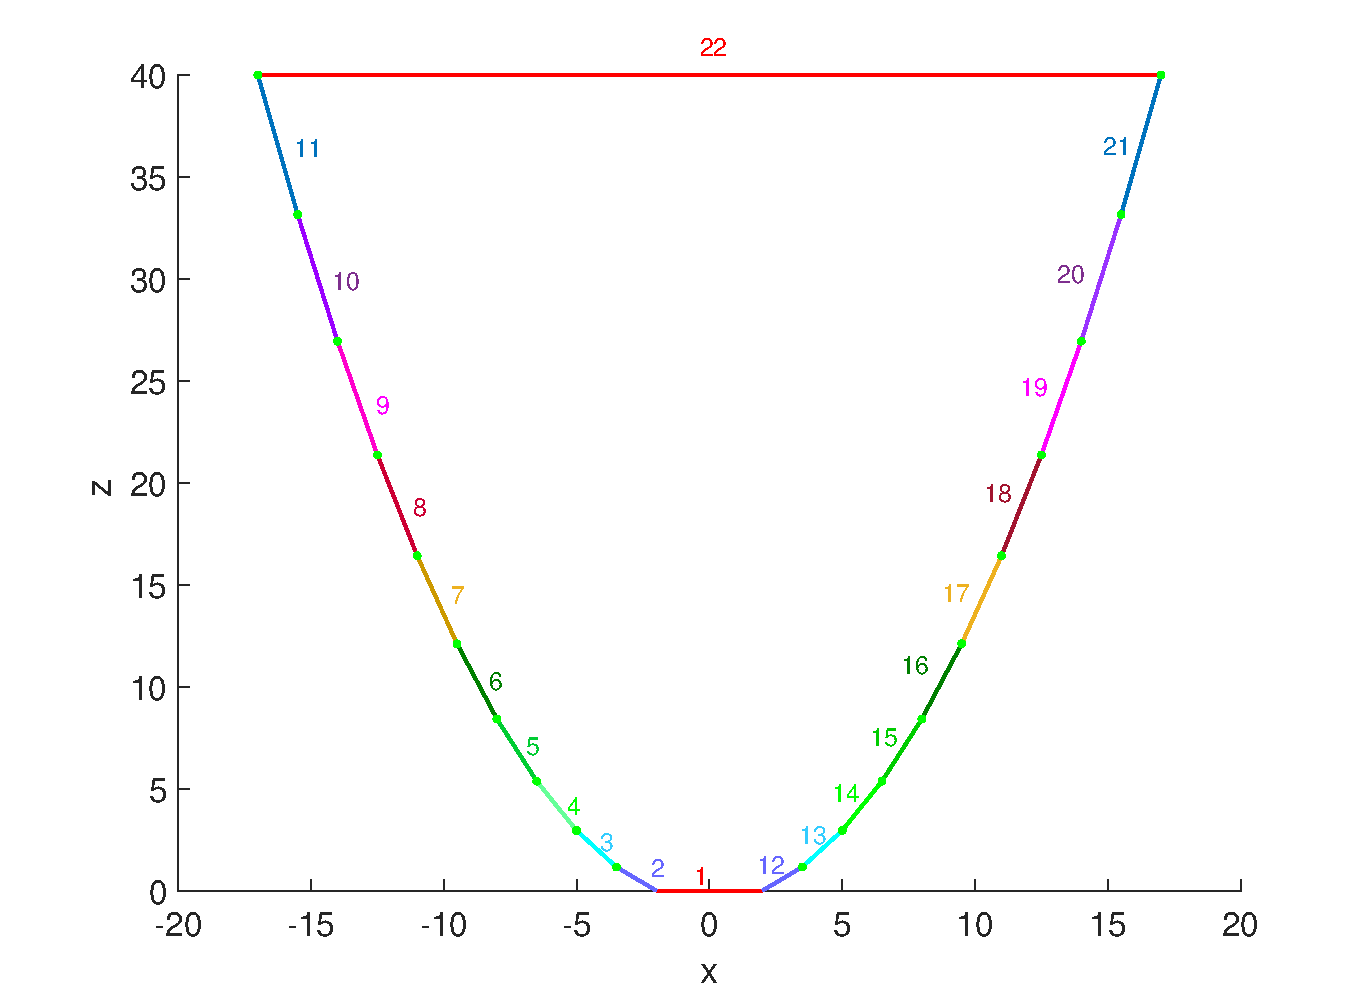
\includegraphics[scale=.4]{multifacetedcup1}
\caption{Shape of the $20$-faceted cup. The system is formed by $22$ different line segments: the source $\point{S}$, the target
$\point{T}$, $10$ left reflectors and $10$ right reflectors.
 $\point{S}=[-2,2]$ is located at $\variabile{z}=0$. $\point{T} = [-17,17]$ is parallel to the source and it is located at a height $\variabile{z}=40$.
 The \variabile{x}-coordinates of the extremes of the reflectors are equidistributed.
 The \variabile{z}-coordinates are on a parabola that passes through the end points of the target and has as symmetry axis the \variabile{z}-axis.
 All the lines are located in air.}
\label{fig:multifacetedcup}
\end{figure}
\\ \indent
Similarly to the two-faceted cup, also for the multi-faceted cup we define the phase spaces of all the lines $\lineai\in\{1, \cdots, \textrm{Nl}\}$ as in Section \ref{sec:algorithm}, for the $20$-faceted cup $\textrm{Nl}=22$. Note that we always choose the index of the target equal to the index of the number of lines that form the system $\textrm{Nl}$.
For the system in Figure \ref{fig:multifacetedcup}, $42$ different phase spaces need to be considered.
In general, for a system formed by $\textrm{Nl}$ straight line segments, $2\textrm{Nl}-2$ phase spaces are considered.
For all the systems formed by straight line segments, the boundaries $(\partial\mbox{\set{S}{\lineai,}{\lineaj}})_{\lineai\neq\lineaj=2, \cdots, \textrm{Nl}}$ and $(\partial\mbox{\set{T}{\lineai,}{\lineak}})_{\lineai\neq\lineak=1, \cdots, \textrm{Nl}-1}$ of the regions that form every PS can be determined as explained in Section \ref{sec:appendix}. \\
\indent The boundaries $(\partial\mbox{\set{T}{\textrm{Nl},}{\lineak}})_{\lineak=1, \cdots, \textrm{Nl}-1}$ for the $20$-faceted cup are depicted in Fig. \ref{fig:T20} with red lines.
\begin{figure}[h]
\centering
\label{fig:T20}
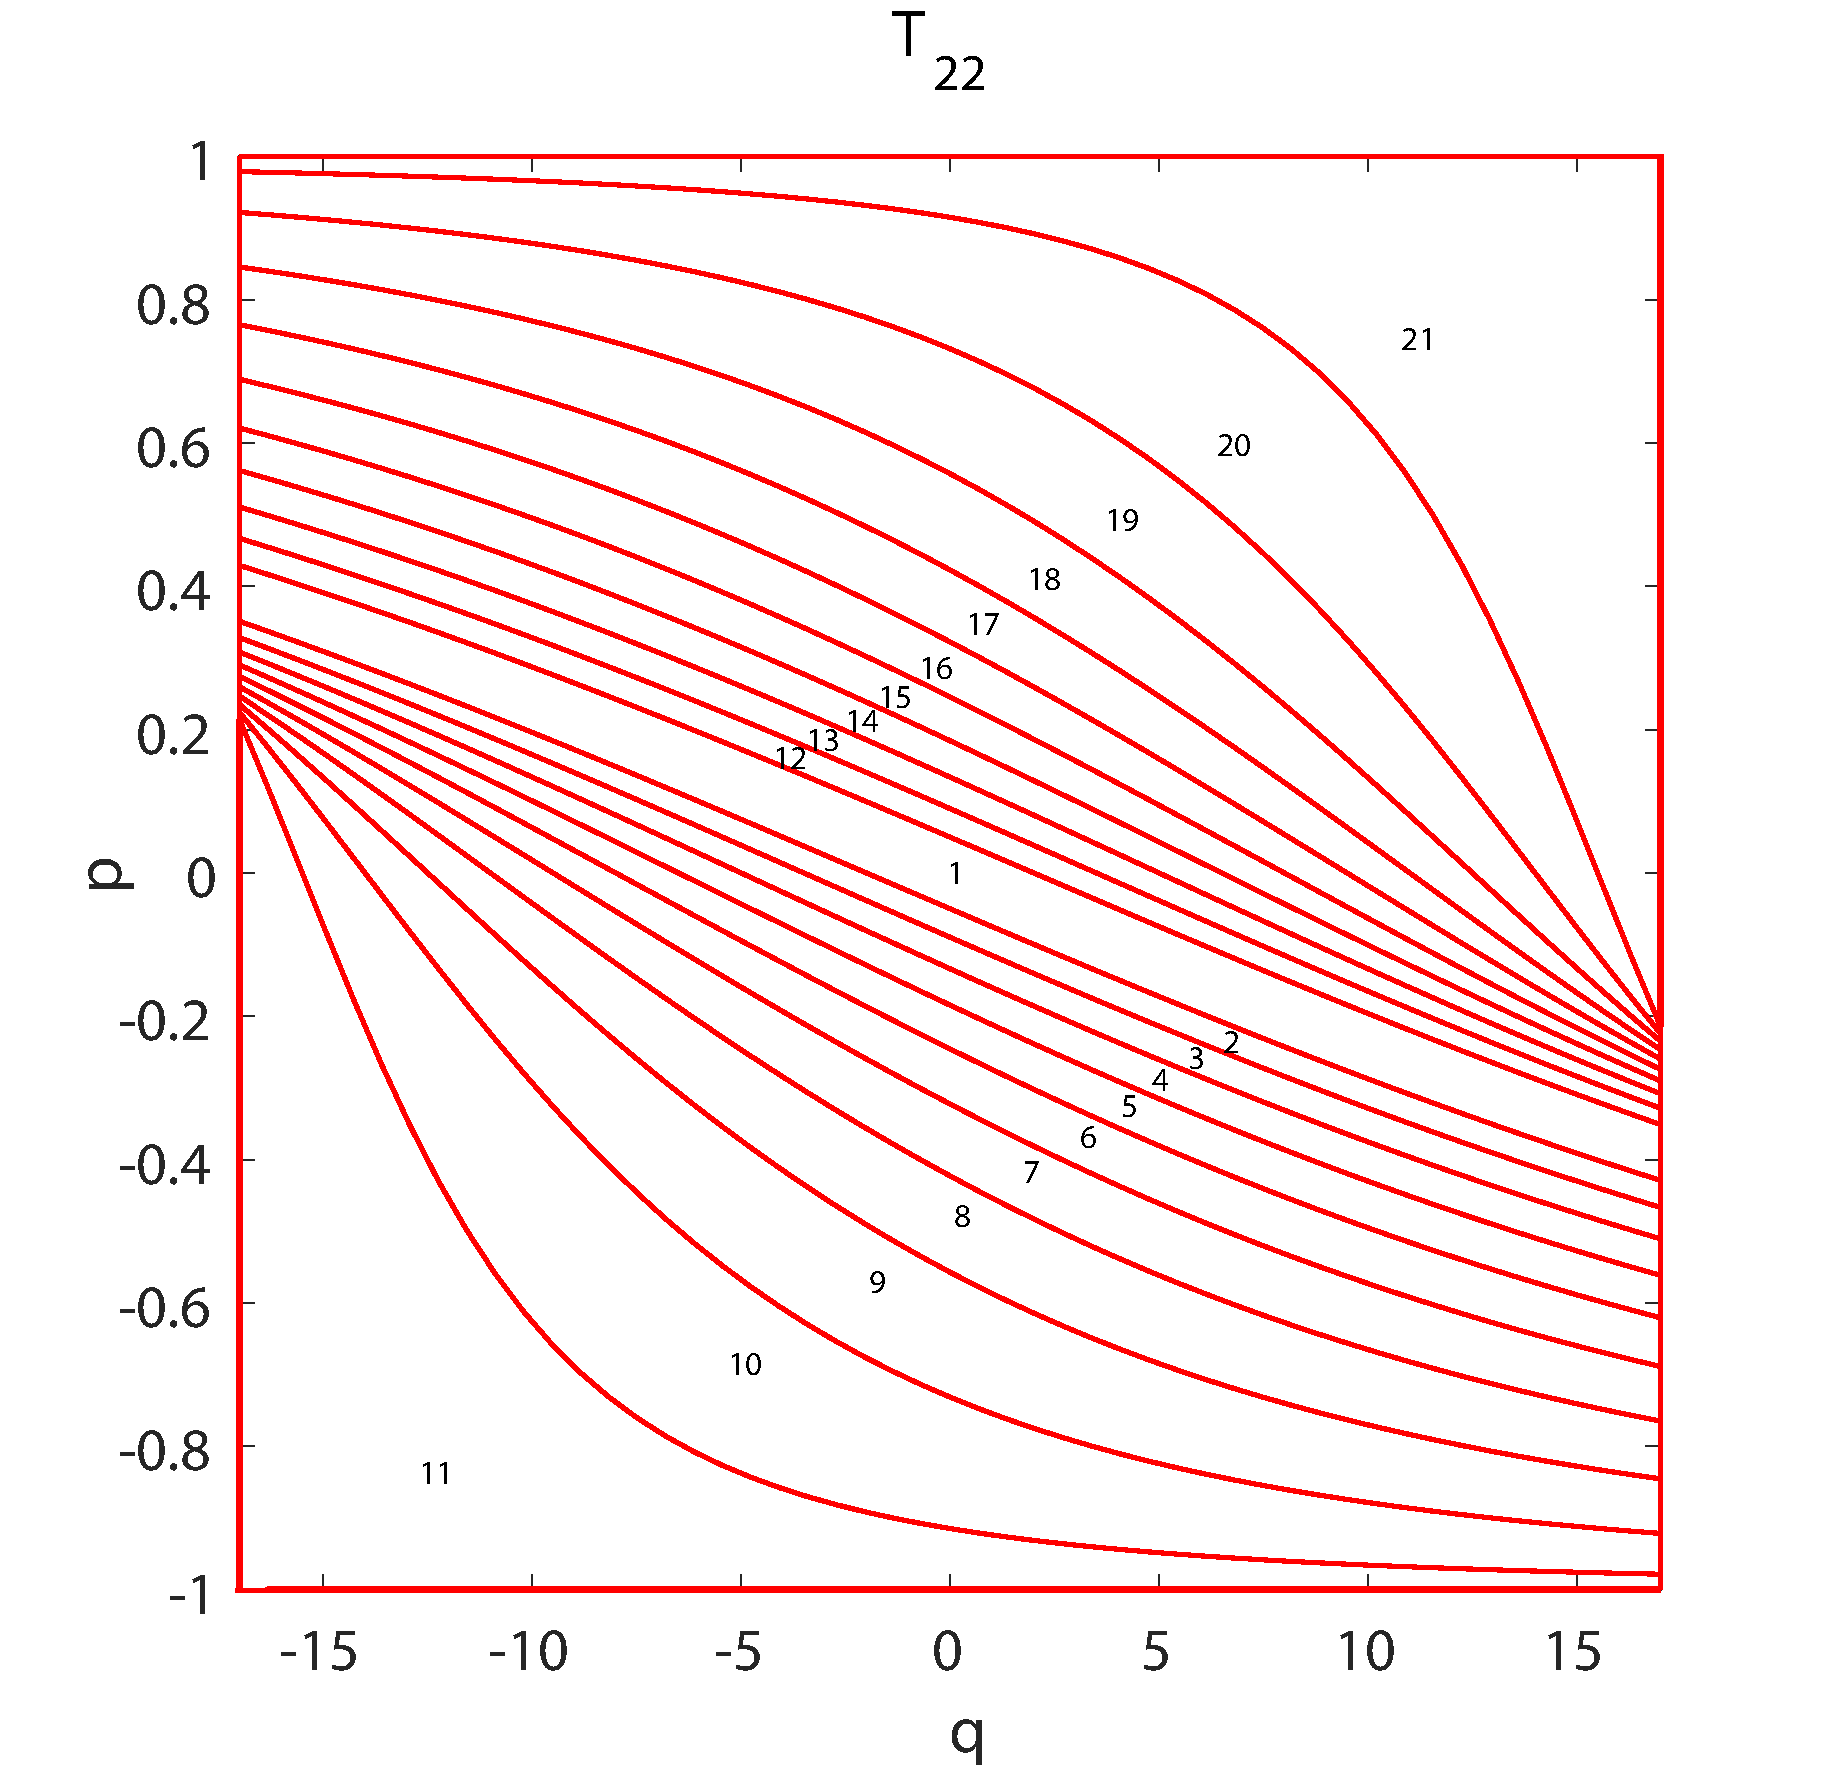
\includegraphics[scale=.35]{target10facetedcup1}
\caption{\textbf{Target phase space of the $20$-faceted cup.}
The red lines are the boundaries $(\partial\mbox{\set{T}{$22$,}{\lineak}})_{\lineak=1, \cdots, 21}$ which are determined analytically. The numbers inside the regions \set{T}{$22$,}{\lineak} indicate the value of the index \lineak.}
\label{fig:T20}
\end{figure}
All the possible paths that the rays can follow when propagating within the $20$-faceted cup are determined using the same algorithm developed for the two-faceted cup and explained in Section \ref{sec:algorithm}.
 As the number of optical lines increases, the number of possible paths increases as well.
 Therefore, we have to construct a more complicated tree than the one in Fig. \ref{fig:tree}.
Despite this, the algorithm explained in the previous section still works fine and, also for the multi-faceted cup we are able to determine all the possible paths $\Pi$ and all the regions \set{R}{}{}$(\Pi)$ with positive luminance at target PS \set{T}{\textrm{Nl}}{}.
Assuming a Lambertian source, only the rays located at the boundaries of these regions need to be computed.
Therefore, for a given direction $\variabile{p}=\const{const}$ only the position coordinates $\variabile{q}^\textrm{\,min}(\Pi,\variabile{p})$ and $\variabile{q}^\textrm{\,max}(\Pi,\variabile{p})$ of the intersection points between the boundaries $ \partial$\set{R}{}{}($\Pi$) and the line $\variabile{p}= const$ are needed for every possible path $\Pi$. Finally, the target intensity $I_{\textrm{PS}}(\variabile{p})$ along the direction $\variabile{p}$ is obtained employing Eq. (\ref{eq:intensity}).
Numerical results for a $20$-faceted cup are given in the next section.
\section{Numerical results for the $20$-faceted cup}
\label{sec:Numerical results_10cup}
In this section the results for the $20$-faceted cup are presented.
We compute the target intensity both with the inverse ray mapping method and MC ray tracing.
The same partitioning $P$ of the interval $[-1,1]$ used for the two-faceted cup is considered.
The normalized MC intensity and
the normalized PS intensity $ \hat{I}_{\textrm{PS}}$ are computed.
Their profiles are depicted in Fig. \ref{fig:intensity10cup} with a blue line and a green dotted line, respectively.
They are compared with a reference intensity $\hat{I}_{\textrm{ref}}$ (red line) which is computed using MC ray tracing with $10^8$ rays.
\begin{figure}[h!]
\centering
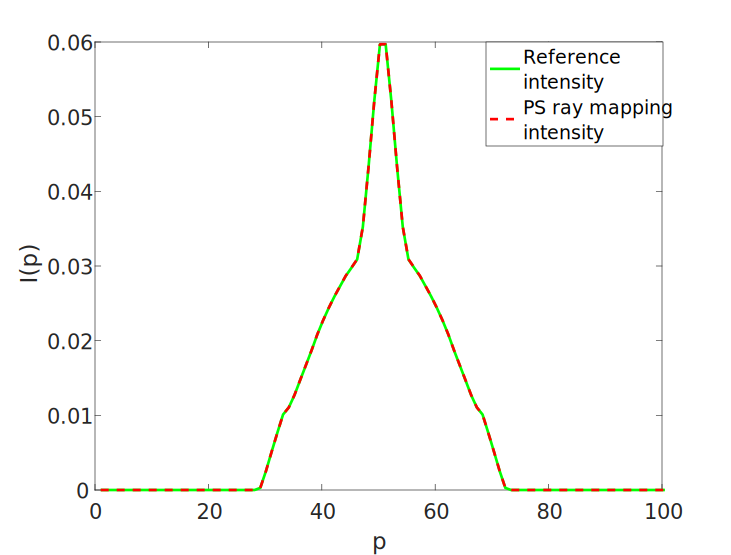
\includegraphics[scale=.4]{intensity_10_cup_raymapping}
\caption{Intensity for the $20$-faceted cup.
The red line shows the reference intensity computed using MC ray tracing with $10^8$ rays.
The blue line depicts the MC intensity with $10^7$ rays.
The green and dotted line shows the intensity found with the ray mapping method.}
\label{fig:intensity10cup}
\end{figure}
\begin{figure}[h!]
\centering
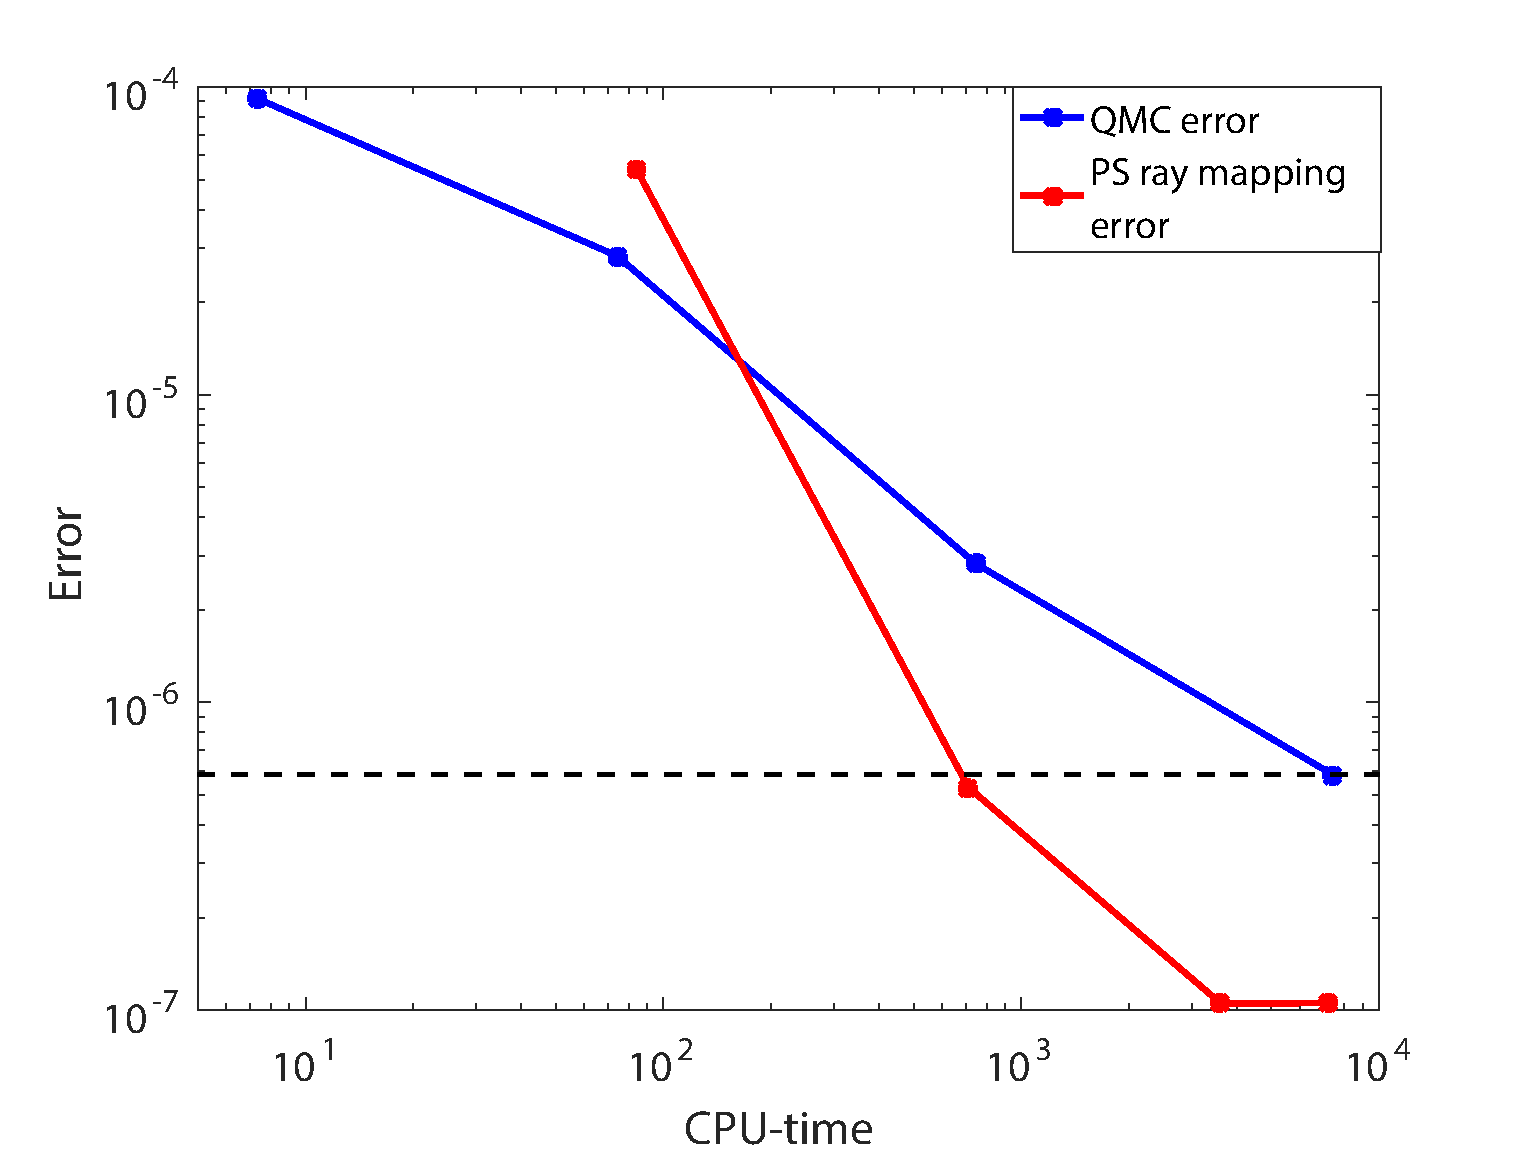
\includegraphics[scale=.4]{error_10_cup_raymapping}
\caption{\textbf{Errors for the $20$-faceted cup as a function of the CPU.} The ray mapping method is more accurate than QMC ray tracing and it is faster in case an error smaller than, say $10^{-4}$, is desired.}
\label{fig:error10cup} 
\end{figure}
Note that the intensity profile in Fig. \ref{fig:intensity10cup} is more concentrated around the direction $\variabile{p}=0$ than the intensity of the two-faceted cup (see Fig. \ref{fig:intensity_cup}). In particular, increasing the number of left and right reflectors the intensity profile becomes more and more peaked around the center approaching the profile of a parabolic reflector, (see \cite{filosa2017}).
\\ \indent In order to show the performance of the new method, we calculate the error between the approximate intensities $\hat{I}_{\textrm{A}}$ ($\textrm{A} = \textrm{MC}, \textrm{PS}$) and the reference intensity $\hat{I}_{\textrm{ref}}$ from Eq. (\ref{error}). In Fig. \ref{fig:error10cup} the speed of convergence for MC ray tracing is shown in blue. 
The better accuracy (the right most red point in Fig. \ref{fig:error10cup}) is obtained tracing $10^8$ rays. Also, the PS intensity is computed several times increasing every time the number of bins used in the trapezoidal rule to approximate the
integrals in Eq. (\ref{eq:intensity}). This has to be done in order to find the averaged PS intensity $\hat{I}_{\textrm{PS}}$ over every bin. The error for the ray mapping method is calculated for all the approximated intensities.
Increasing the number of bins in the trapezoidal rule, the PS error decreases. 
We remark that the PS method gives the value of the intensity pointwise, therefore we can compute the PS intensity without numeric integration. Nevertheless, we calculate the averaged intensity because we want to compare it with the MC intensity $\hat{I}_{\textrm{MC}}$.
\\ \indent The error convergence is depicted in Fig. \ref{fig:error10cup} with the red line.
Since all the boundaries of the regions in PS are calculated exactly, the PS intensity is analytic.
From Fig. \ref{fig:error10cup} we observe that the minimum difference between the reference intensity and the approximated intensity found with the ray mapping method has an order of magnitude of $10^{-6}$.
This is due to the fact that for the $20$-faceted cup the intensity cannot be computed exactly. 
Therefore, we took as reference intensity an intensity computed with MC ray tracing using $7.5*10^8$ rays which is not the exactly intensity.
The error between the normalized exact intensity $\hat{I}_{\textrm{exact}}$ and the normalized approximate intensity $\hat{I}_{\textrm{A}}$ is given by:
\begin{equation}
\frac{1}{\textrm{Nb}}\sum_{\variabile{h} = 1}^{\textrm{Nb}}| \hat{I}_{\textrm{exact}}(\variabile{p}^\variabile{h}) - \hat{I}_{\textrm{A}}(\variabile{p}^\variabile{h})| \leq
\frac{1}{\textrm{Nb}}\Bigg(\sum_{\variabile{h} = 1}^{\textrm{Nb}}\big| \hat{I}_{\textrm{exact}}(\variabile{p}^\variabile{h}) - \hat{I}_{\textrm{ref}}(\variabile{p}^\variabile{h})\big| +
\sum_{\variabile{h} = 1}^{\textrm{Nb}}\big| \hat{I}_{\textrm{ref}}(\variabile{p}^\variabile{h}) - \hat{I}_{\textrm{A}}(\variabile{p}^\variabile{h})\big|\Bigg)\,.
\end{equation}
Extrapolating the MC error we obtain an approximation of the difference between the reference solution (MC ray tracing with $7.5*10^{8}$ rays) and the exact intensity,
this error is depicted in Fig. \ref{fig:error10cup} with the cyan dot.
From numerical symulation we obtain the difference between the extrapolated value and the exact intensity 
\begin{equation*}\sum_{\variabile{h} = 1}^{\textrm{Nb}}| \hat{I}_{\textrm{exact}}(\variabile{p}^\variabile{h}) - \hat{I}_{\textrm{ref}}(\variabile{p}^\variabile{h})|/\textrm{Nb}\approx 1.68*10^{-6}, \end{equation*} where $\textrm{Nb}=100$
The results show that 
\begin{equation*}
\sum_{\variabile{h} = 1}^{\textrm{Nb}}| \hat{I}_{\textrm{exact}}(\variabile{p}^\variabile{h}) - \hat{I}_{\textrm{ref}}(\variabile{p}^\variabile{h})|/\textrm{Nb}
\approx \sum_{\variabile{h} = 1}^{\textrm{Nb}}|\hat{I}_{\textrm{ref}}(\variabile{p}^\variabile{h}) - \hat{I}_{\textrm{PS}}(\variabile{p}^\variabile{h})|/\textrm{Nb}.
\end{equation*}
Therefore, we claim that the error found with the inverse ray mapping method is also due to the MC error.
We can conclude that the inverse ray mapping method performs very well also for more complicated systems.
Compared to MC ray tracing the new method is not only faster but also much more accurate.
\section{Discussions}
In this chapter, we presented an inverse method to compute the intensity of light emitted by the source and received by the target of a given optical system.
We tested our method for two-dimensional optical systems formed by straight line segments.
The method employs the phase spaces of \textit{all} the lines that form the system.
All these phase spaces are related to each other through two different kinds of maps.
A concatenation of these two maps gives a map that connects the coordinates of the rays at the source with those at the target.
Employing the inverse of the concatenated map, all the possible paths that rays can follow during their propagation are found. 
Only the rays located on the boundaries of the regions with positive luminance are traced,
where every region is formed by rays that follow the same path during their propagation. 
Assuming constant luminance, only these rays are needed to calculate the output intensity. \\ \indent
We presented numerical results for a simple system: the two-faceted cup. We employ the PS of all the lines that form the system, 
each of them is divided into regions the boundaries of which are determined exactly.
 Numerical results show that the exactly output intensity is found.
 We compared our method with MC ray tracing showing significant advantages in terms of the accuracy and the computational time.
 \\ \indent Then, we explained how the method can be extended to more complicated optical systems.
We took as an example a system with $10$ left and $10$ right segments as reflectors, the so-called $20$-faceted cup.
Also for the generalized system, the boundaries of the regions that form every PS are determined exactly. This is true for all the systems formed by straight lines.
This allows finding the analytic output intensity.
To validate our method, the intensity found using the new technique is compared with the MC intensity.
To demonstrate both the accuracy and speed advantages, numerical results are presented also for the $20$-faceted cup.















